\documentclass[10pt,a4paper]{article}
\usepackage[UTF8,fontset = windows]{ctex}
\setCJKmainfont[BoldFont=黑体,ItalicFont=楷体]{华文中宋}
\usepackage{amssymb,amsmath,amsfonts,amsthm,mathrsfs,dsfont,graphicx}
\usepackage{ifthen,indentfirst,enumerate,color,titletoc}
\usepackage{tikz}
\usepackage{multicol}
\usepackage{makecell}
\usepackage{longtable}
\usetikzlibrary{arrows,calc,intersections,patterns,decorations.pathreplacing,3d,angles,quotes,positioning}
\usepackage[bf,small,indentafter,pagestyles]{titlesec}
\usepackage[top=1in, bottom=1in,left=0.8in,right=0.8in]{geometry}
\renewcommand{\baselinestretch}{1.65}
\newtheorem{defi}{定义~}
\newtheorem{eg}{例~}
\newtheorem{ex}{~}
\newtheorem{rem}{注~}
\newtheorem{thm}{定理~}
\newtheorem{coro}{推论~}
\newtheorem{axiom}{公理~}
\newtheorem{prop}{性质~}
\newcommand{\blank}[1]{\underline{\hbox to #1pt{}}}
\newcommand{\bracket}[1]{(\hbox to #1pt{})}
\newcommand{\onech}[4]{\par\begin{tabular}{p{.9\textwidth}}
A.~#1\\
B.~#2\\
C.~#3\\
D.~#4
\end{tabular}}
\newcommand{\twoch}[4]{\par\begin{tabular}{p{.46\textwidth}p{.46\textwidth}}
A.~#1& B.~#2\\
C.~#3& D.~#4
\end{tabular}}
\newcommand{\vartwoch}[4]{\par\begin{tabular}{p{.46\textwidth}p{.46\textwidth}}
(1)~#1& (2)~#2\\
(3)~#3& (4)~#4
\end{tabular}}
\newcommand{\fourch}[4]{\par\begin{tabular}{p{.23\textwidth}p{.23\textwidth}p{.23\textwidth}p{.23\textwidth}}
A.~#1 &B.~#2& C.~#3& D.~#4
\end{tabular}}
\newcommand{\varfourch}[4]{\par\begin{tabular}{p{.23\textwidth}p{.23\textwidth}p{.23\textwidth}p{.23\textwidth}}
(1)~#1 &(2)~#2& (3)~#3& (4)~#4
\end{tabular}}
\begin{document}

\begin{enumerate}[1.]

\item {\tiny (000048)}填空题:\\
(1) 若$x^3=5$, 则$x=$\blank{50}; 若$3^x=5$, 则$x=$\blank{50}.\\
(2) 将$\sqrt[4]{a\sqrt[3]{a}} \ (a>0)$化成有理数指数幂的形式为\blank{50}.\\
(3) 若$\log_8x=-\dfrac 23$, 则$x=$\blank{50}.\\
(4) 若$\log_a b\cdot \log_5 a=3$($a>0$且$a\ne 1$), 则$b=$\blank{50}.
\item {\tiny (000049)}选择题:\\
(1) 若$\lg a$与$\lg b$互为相反数, 则有\bracket{20}.
\fourch{$a+b=0$}{$ab=1$}{$\dfrac ab=1$}{以上答案均不对}
(2) 设$a>0$, 下列计算中正确的是\bracket{20}.
\twoch{$a^\frac{2}{3}\cdot a^\frac{3}{2}=a$}{$a^\frac{2}{3}\div a^\frac{3}{2}=a$}{$a^{-4}\cdot a^4=0$}{$(a^\frac{2}{3})^\frac{3}{2}=a$}
\item {\tiny (000051)}求下列各式的值:\\
(1) $\dfrac{1}{4^x+1}+\dfrac{1}{4^{-x}+1}$;\\
(2) $4^{\sqrt 2+1}\times 2^{3-2\sqrt 2}\times 8^{-\frac 23}$.
\item {\tiny (000052)}已知$\lg a<1$, 化简$\sqrt{\lg^2 a-\lg \dfrac{a^2}{10}}$.
\item {\tiny (000053)}已知$m=\log_2 10$, 求$2^m-m\lg 2-4$的值.
\item {\tiny (000054)}填空题:\\
(1) 若$4^x=2^{-\frac{1}{2}}$, $4^y=\sqrt[3]{32}$, 则$2x-3y=$\blank{50}.\\
(2) 若$\log_3(\log_4 x)=1$, 则$x=$\blank{50}.\\
(3) 若$3^a=7^b=63$, 则$\dfrac 2a+\dfrac 1b$的值为\blank{50}.\\
\item {\tiny (000055)}已知$\log_{18}9=a$, $18^b=5$, 则$\log_{36}45$等于\bracket{20}.
\fourch{$\dfrac{a+b}{2+a}$}{$\dfrac{a+b}{2-a}$}{$\dfrac{a+b}{2a}$}{$\dfrac{a+b}{a^2}$}
\item {\tiny (000056)}设$\log_{0.2}a>0$, $\log_{0.2}b>0$, 且$\log_{0.2}a\cdot \log_{0.2}b=1$, 求$\log_{0.2}(ab)$的最小值.
\item {\tiny (000057)}化简$\dfrac{(1+2^x)(1+2^{2x})(1+2^{4x})(1+2^{8x})(1+2^{16x})}{1-2^{32x}}$(其中$x\ne 0$).
\item {\tiny (000058)}已知$a>1$, $b>0$. 求证: 对任意给定的实数$k$, $a^{2b+k}-a^{b+k}>a^{b+k}-a^k$.
\item {\tiny (000059)}甲、乙两人同时解关于$x$的方程: $\log_2x+b+c\log_x2=0$. 甲写错了常数$b$, 得两根
$\dfrac 14$及$\dfrac 18$; 乙写错了常数$c$, 得两根$\dfrac 12$及$64$. 求这个方程的真正根.
\item {\tiny (000060)}已知$a$、$b$及$c$是不为$1$的正数, 且$\lg a+\lg b+\lg c=0$. 求证: $a^{\frac{1}{\lg b}+\frac{1}{\lg c}}\cdot b^{\frac{1}{\lg c}+\frac{1}{\lg a}}\cdot c^{\frac{1}{\lg a}+\frac{1}{\lg b}}=\dfrac{1}{1000}$.
\item {\tiny (000061)}填空题:\\
(1) 若点$(2, \sqrt 2)$在幂函数$y=x^a$的图像上, 则该幂函数的表达式为\blank{50}; 若点$(2, \sqrt 2)$在指数函数$y=a^x$($a>0$且$a\ne 1$)的图像上, 则该指数函数的表达式为\blank{50}; 若点$(\sqrt 2, 2)$在对数函数$y=\log_a x$($a>0$且$a\ne 1$)的图像上, 则该对数
函数的表达式为\blank{50}.\\
(2) 若幂函数$y=x^k$在区间$(0, +\infty)$上是严格减函数, 则实数$k$的取值范围为\blank{50}.\\
(3) 已知常数$a>0$且$a\ne 1$, 假设无论$a$为何值, 函数$y=a^{x-2}+1$的图像恒经过一
个定点. 则这个点的坐标为\blank{50}.
\item {\tiny (000062)}选择题:\\
(1) 若指数函数$y=a^x$($a>0$且$a\ne 1$)在$\mathbf{R}$上是严格减函数, 则下列不等式中, 一定能成立的是\bracket{20}.
\fourch{$a>1$}{$a<0$}{$a(a-1)<0$}{$a(a-1)>0$}
(2) 在同一平面直角坐标系中, 一次函数$y=x+a$与对数函数$y=\log_ax$($a>0$且$a\ne 1$)的图像关系可能是\bracket{20}.
\fourch{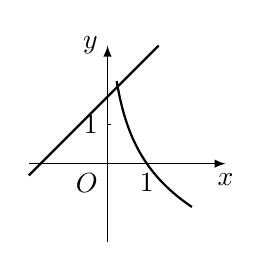
\begin{tikzpicture}[scale = 0.5,>=latex]
    \draw [->] (-2,0) -- (3,0) node [below] {$x$};
    \draw [->] (0,-2) -- (0,3) node [left] {$y$};
    \draw (0,0) node [below left] {$O$};
    \draw (0.1,1) -- (0,1) node [left] {$1$};
    \draw (1,0) node [below] {$1$};
    \draw [thick] (-2,-0.3) -- (1.3,3);
    \draw [thick,domain =-1.1:2.1,samples = 200] plot ({0.5^\x},\x);
\end{tikzpicture}
}{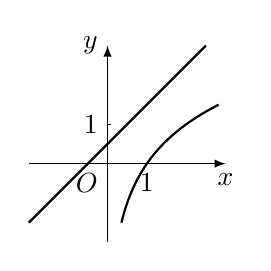
\begin{tikzpicture}[scale = 0.5,>=latex]
    \draw [->] (-2,0) -- (3,0) node [below] {$x$};
    \draw [->] (0,-2) -- (0,3) node [left] {$y$};
    \draw (0,0) node [below left] {$O$};
    \draw (0.1,1) -- (0,1) node [left] {$1$};
    \draw (1,0) node [below] {$1$};
    \draw [thick] (-2,-1.5) -- (2.5,3);
    \draw [thick,domain =1.5:-1.5,samples = 200] plot ({0.5^\x},-\x);
\end{tikzpicture}
}{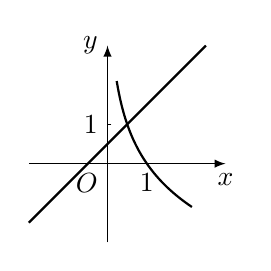
\begin{tikzpicture}[scale = 0.5,>=latex]
    \draw [->] (-2,0) -- (3,0) node [below] {$x$};
    \draw [->] (0,-2) -- (0,3) node [left] {$y$};
    \draw (0,0) node [below left] {$O$};
    \draw (0.1,1) -- (0,1) node [left] {$1$};
    \draw (1,0) node [below] {$1$};
    \draw [thick] (-2,-1.5) -- (2.5,3);
    \draw [thick,domain =-1.1:2.1,samples = 200] plot ({0.5^\x},\x);
\end{tikzpicture}
}{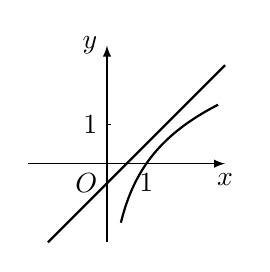
\begin{tikzpicture}[scale = 0.5,>=latex]
    \draw [->] (-2,0) -- (3,0) node [below] {$x$};
    \draw [->] (0,-2) -- (0,3) node [left] {$y$};
    \draw (0,0) node [below left] {$O$};
    \draw (0.1,1) -- (0,1) node [left] {$1$};
    \draw (1,0) node [below] {$1$};
    \draw [thick] (-1.5,-2) -- (3,2.5);
    \draw [thick,domain =1.5:-1.5,samples = 200] plot ({0.5^\x},-\x);
\end{tikzpicture}
}
\item {\tiny (000063)}求下列函数的的定义域:\\
(1) $y=(x-1)^{\frac 52}$;\\
(2) $y=3^{\sqrt{x-1}}$;\\
(3) $y=\lg \dfrac{1+x}{1-x}$.
\item {\tiny (000064)}比较下列各题中两个数的大小:\\
(1) $0.1^{0.7}$与$0.2^{0.7}$;\\
(2) $0.7^{0.1}$与$0.7^{0.2}$;\\
(3) $\log_{0.7}0.1$与$\log_{0.7}0.2$.
\item {\tiny (000065)}设点$(\sqrt 2, 2)$在幂函数$y_1=x^a$的图像上, 点$(-2,\dfrac 14)$在幂函数$y_2=x^b$的图像上. 当$x$取何值时, $y_1=y_2$?
\item {\tiny (000066)}设$a=(\dfrac 23)^x$, $b=x^{\frac 32}$及$c=\log_\frac{2}{3}x$, 当$x>1$时, 试比较$a$、$b$及$c$之间的大小关系.
\item {\tiny (000067)}设常数$a>0$且$a\ne 1$, 若函数$y=\log_a(x+1)$在区间$[0, 1]$上的最大值为$1$, 最小值为$0$, 求实数$a$的值.
\item {\tiny (000069)}填空题:\\
(1) 已知$m\in \mathbf{Z}$, 设幂函数$y=x^{m^2-4m}$的图像关于原点成中心对称, 且与$x$轴及$y$轴均无交点, 则$m$的值为\blank{50}.\\
(2) 设$a$、$b$为常数, 若$0<a<1$, $b<-1$, 则函数$y=a^x+b$的图像必定不经过第\blank{50}象限.
\item {\tiny (000070)}选择题:\\
(1) 若$m>n>1$, 而$0<x<1$, 则下列不等式正确的是\bracket{20}.
\fourch{$m^x<n^x$}{$x^m<x^n$}{$\log_x m>\log_x n$}{$\log_m x<\log_n x$}
(2) 在同一平面直角坐标系中, 二次函数$y=ax^2+bx$与指数函数$y=(\dfrac ba)^x$的图像关系可能为\bracket{20}.
\fourch{
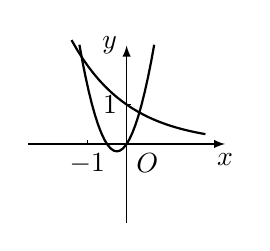
\begin{tikzpicture}[scale = 0.5, >=latex]
    \draw [->] (-2.5,0) -- (2.5,0) node [below] {$x$};
    \draw [->] (0,-2.) -- (0,2.5) node [left] {$y$};
    \draw (0,0) node [below right] {$O$};
    \draw (-1,0.1) -- (-1,0) node [below] {$-1$};
    \draw (0.1,1) -- (0,1) node [left] {$1$};
    \draw [domain = -1.2:0.7,thick] plot (\x,{3*\x * (\x+0.5)});
    \draw [domain = -1.4:2,thick] plot (\x,{(0.5)^\x}); 
\end{tikzpicture}
}{
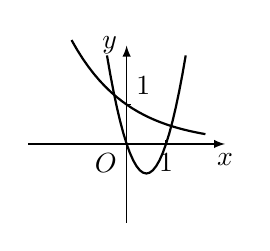
\begin{tikzpicture}[scale = 0.5, >=latex]
    \draw [->] (-2.5,0) -- (2.5,0) node [below] {$x$};
    \draw [->] (0,-2.) -- (0,2.5) node [left] {$y$};
    \draw (0,0) node [below left] {$O$};
    \draw (1,0.1) -- (1,0) node [below] {$1$};
    \draw (0.1,1) -- (0,1) node [above right] {$1$};
    \draw [domain = -0.5:1.5,thick] plot (\x,{3*\x*(\x-1)});
    \draw [domain = -1.4:2,thick] plot (\x,{(0.5)^\x}); 
\end{tikzpicture}
}{
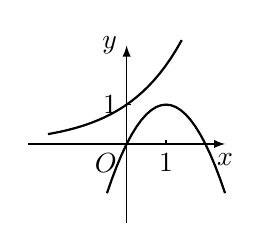
\begin{tikzpicture}[scale = 0.5, >=latex]
    \draw [->] (-2.5,0) -- (2.5,0) node [below] {$x$};
    \draw [->] (0,-2.) -- (0,2.5) node [left] {$y$};
    \draw (0,0) node [below left] {$O$};
    \draw (1,0.1) -- (1,0) node [below] {$1$};
    \draw (0.1,1) -- (0,1) node [left] {$1$};
    \draw [domain = -0.5:2.5,thick] plot ({\x},{-\x*(\x-2)});
    \draw [domain = -1.4:2,thick] plot ({-\x},{(0.5)^\x}); 
\end{tikzpicture}
}{
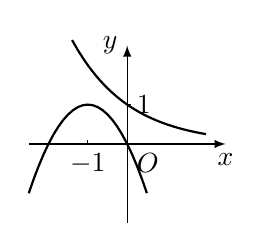
\begin{tikzpicture}[scale = 0.5, >=latex]
    \draw [->] (-2.5,0) -- (2.5,0) node [below] {$x$};
    \draw [->] (0,-2.) -- (0,2.5) node [left] {$y$};
    \draw (0,0) node [below right] {$O$};
    \draw (-1,0.1) -- (-1,0) node [below] {$-1$};
    \draw (0.1,1) -- (0,1) node [right] {$1$};
    \draw [domain = -2.5:0.5,thick] plot ({\x},{-\x*(\x+2)});
    \draw [domain = -1.4:2,thick] plot ({\x},{(0.5)^\x}); 
\end{tikzpicture}   
}
\item {\tiny (000071)}设$a$为常数且$0<a<1$, 若$y=(\log_a \dfrac 35)^x$在$\mathbf{R}$上是严格增函数, 求实数$a$的取值范围.
\item {\tiny (000072)}在同一平面直角坐标系中, 作出函数$y=(\dfrac 12)^x$及$y=x^{\frac 12}$的大致图像, 并求方程$(\dfrac 12)^x=x^{\frac 12}$的解的个数.
\item {\tiny (000073)}已知集合$A=\{y|y=(\dfrac 12)^x,\  x\in [-2, 0)\}$, 用列举法表示集合$B=\{y|y=\log_3x,\  x\in A\text{且}y\in \mathbf{Z}\}$.
\item {\tiny (000074)}$\log_23$是有理数吗? 请证明你的结论.
\item {\tiny (000075)}仅利用对数函数的单调性和计算器上的乘方功能来确定对数$\log_23$第二位小数的值.
\item {\tiny (000330)}若函数$f(x)=\log_2\dfrac{x-a}{x+1}$的反函数的图像过点$(-2,3)$, 则$a=$\blank{50}.
\item {\tiny (000342)}若函数$f(x)=\begin{cases}    2^x, & x\le 0, \\ -x^2+m, & x>0 \end{cases}$的值域为$(-\infty ,1]$, 则实数$m$的取值范围是\blank{50}.
\item {\tiny (000344)}定义在$\mathbf{R}$上的偶函数$y=f(x)$, 当$x\ge 0$时, $f(x)=\lg (x^2-3x+3)$, 则$f(x)$在$\mathbf{R}$上的零点个数为\blank{50}个.
\item {\tiny (000349)}若函数$f(x)=\log_2 (x+1)+a$的反函数的图像经过点$(4,1)$, 则实数$a=$\blank{50}.
\item {\tiny (000358)}函数$f(x)=1+\log_2 x$($x\ge 1$)的反函数$f^{-1}(x)=$\blank{50}.
\item {\tiny (000362)}方程$\log_2(9^x-5)=2+\log_2(3^x-2)$的解$x=$\blank{50}.
\item {\tiny (000367)}设函数$f(x)=\begin{cases}\log_2 x, & x>0, \\ 4^x, & x\le 0,\end{cases}$ 则$f(f(-1))=$\blank{50}.
\item {\tiny (000381)}若点$(8,4)$在函数$f(x)=1+\log_a x$图像上, 则$f(x)$的反函数为\blank{50}.
\item {\tiny (000388)}已知函数$f(x)=a^x-1$的图像经过$(1,1)$点, 则$f^{-1}(3)=$\blank{50}.
\item {\tiny (000406)}方程$\lg (3x+4)=1$的解$x=$\blank{50}.
\item {\tiny (000425)}若关于$x$的不等式$|2^x-m|-\dfrac1{2^x}<0$在区间$[0,1]$内恒成立, 则实数$m$的范围\blank{50}.
\item {\tiny (000450)}函数$f(x)=2^x+m$的反函数为$y=f^{-1}(x)$, 且$y=f^{-1}(x)$的图像过点$Q(5,2)$, 那么$m=$\blank{50}.
\item {\tiny (000472)}若函数$f(x)=x^a$的反函数的图像经过点$(\dfrac12,\dfrac14)$, 则$a=$\blank{50}.
\item {\tiny (000474)}已知函数$y=f(x)$是奇函数, 当$x<0$时, $f(x)=2^x-ax$, 且$f(2)=2$, 则$a=$\blank{50}.
\item {\tiny (000486)}函数$f(x)=\lg(2-x)$的定义域是\blank{50}.
\item {\tiny (000495)}已知函数$f(x)=\begin{cases} 2^x, & x\le 0, \\ f(x-2), & x>0, \end{cases}$ 则$f(1)+f(2)+f(3)+\cdots+f(2017)=$\blank{50}.
\item {\tiny (000498)}已知幂函数的图像过点$(2,\dfrac14)$, 则该幂函数的单调递增区间是\blank{50}.
\item {\tiny (000520)}已知函数$f(x)=a\cdot 2^x+3-a\ (a\in \mathbf{R})$的反函数为$y=f^{-1}(x)$, 则函数$y=f^{-1}(x)$的图像经过的定点的坐标为\blank{50}.
\item {\tiny (000525)}已知函数$f(x)=\begin{cases} (5-a)x+1, & x<1, \\ a^x, & x\ge 1\end{cases} \ (a>0,a\ne 1)$是实数集$\mathbf{R}$上的增函数, 则实数$a$的取值范围为\blank{50}.
\item {\tiny (000538)}方程$\log_2(2-x)+\log_2(3-x)=\log_2 12$的解$x=$\blank{50}.
\item {\tiny (000549)}已知函数$f(x)=\log_2(x+a)$的反函数为$y=f^{-1}(x)$, 且$f^{-1}(2)=1$, 则实数$a=$\blank{50}.
\item {\tiny (000565)}已知函数$f(x)=\begin{cases} \log_2 (x+a), & x\le 0, \\ x^2-3ax+a, & x>0 \end{cases}$有三个不同的零点, 则实数$a$的取值范围是\blank{50}.
\item {\tiny (000567)}函数$f(x)=\sqrt{1-\lg x}$的定义域为\blank{50}.
\item {\tiny (000582)}数列$\{a_n\}$的前$n$项和为$S_n$, 若点$(n,S_n) \ (n\in \mathbf{N}^*)$在函数$y=\log_2 (x+1)$的反函数的图像上, 则$a_n$=\blank{50}.
\item {\tiny (000590)}已知函数$f(x)=1+\log_a x$, $y=f^{-1}(x)$是函数$y=f(x)$的反函数, 若$y=f^{-1}(x)$的图像过点$(2,4)$, 则$a$的值为\blank{50}.
\item {\tiny (000594)}已知函数$f(x)$是定义在$\mathbf{R}$上且周期为$4$的偶函数. 当$x\in [2,4]$时, $f(x)=\left|\log_4(x-\dfrac32)\right|$, 则$f(\dfrac12)$的值为\blank{50}.
\item {\tiny (000604)}已知函数$f(x)=\begin{cases} \log_2 x, & 0<x<2, \\ (\dfrac23)^x+\dfrac59, & x\ge 2. \end{cases}$ 若函数$g(x)=f(x)-k$有两个不同的零点, 则实数$k$的取值范围是\blank{50}.
\item {\tiny (000607)}函数$y=\log_2(1-\dfrac1x)$的定义域为\blank{50}.
\item {\tiny (000614)}若函数$f(x)=\log_2^2x-\log_2 x+1 \ (x\ge 2)$的反函数为$f^{-1}(x)$, 则$f^{-1}(3)$=\blank{50}.
\item {\tiny (000616)}方程$\log_3(2x+1)=2$的解是\blank{50}.
\item {\tiny (000622)}若函数$f(x)=2^x(x+a)-1$在区间$[0,1]$上有零点, 则实数$a$的取值范围是\blank{50}.
\item {\tiny (000634)}若函数$f(x)=4^x+2^{x+1}$的图像与函数$y=g(x)$的图像关于直线$y=x$对称, 则$g(3)=$\blank{50}.
\item {\tiny (000650)}若函数$f(x)=\begin{cases} -x+3a, & x<0,  \\ a^x+1, & x\ge 0 \end{cases}$($a>0$, 且$a\ne 1$)是$\mathbf{R}$上的减函数, 则$a$的取值范围是\blank{50}.
\item {\tiny (000656)}已知集合$A=\{x|\ln x>0 \}$, $B=\{x|2^x<3\}$, 则\blank{50}.
\item {\tiny (000660)}设$f(x)$为$\mathbf{R}$上的奇函数. 当$x\ge 0$时, $f(x)=2^x+2x+b$($b$为常数), 则$f(-1)$的值为\blank{50}.
\item {\tiny (000675)}已知定义在$\mathbf{R}$上的函数$f(x)$满足: \textcircled{1} $f(x)+f(2-x)=0$; \textcircled{2} $f(x)-f(-2-x)=0$; \textcircled{3} 在$[-1,1]$上的表达式为$f(x)=\begin{cases} \sqrt{1-x^2}, & x\in [-1,0], \\ 1-x, & x\in (0,1] \end{cases}$, 则函数$f(x)$与函数$g(x)=\begin{cases} 2^x, & x\le 0, \\ \log_{\frac12} x,& x>0 \end{cases}$的图像在区间$[-3,3]$上的交点的个数为\blank{50}.
\item {\tiny (000693)}已知函数$f(x)=\begin{cases}2^x, & x\le 0, \\ \log_2 x, & 0<x\le 1\end{cases}$的反函数是$f^{-1}(x)$, 则$f^{-1}(\dfrac12)=$\blank{50}.
\item {\tiny (000702)}设$f(x)$是定义在$\mathbf{R}$上的奇函数, 当$x>0$时,$f(x)=2^x-3$. 则不等式$f(x)<-5$的解为\blank{50}.
\item {\tiny (000724)}设$f(x)$是定义在$\mathbf{R}$上以$2$为周期的偶函数, 当$x\in [0,1]$时, $f(x)=\log_2(x+1)$, 则函数$f(x)$在$[1,2]$上的解析式是\blank{50}.
\item {\tiny (000734)}给出下列函数: \textcircled{1} $y=x+\dfrac1x$; \textcircled{2} $y={x^2}+x$; \textcircled{3} $y={2^{|x|}}$; \textcircled{4} $y={x^{\dfrac23}}$; \textcircled{5} $y=\tan x$; \textcircled{6} $y=\sin(\arccos x)$; \textcircled{7} $y=\lg(x+\sqrt{{x^2}+4})-\lg 2$. 从这$7$个函数中任取两个函数, 则其中一个是奇函数另一个是偶函数的概率是\blank{50}.
\item {\tiny (000738)}函数$f(x)=\lg (3^x-2^x)$的定义域为\blank{50}.
\item {\tiny (000761)}方程$\log_3(3 \cdot 2^x+5)-\log_3(4^x+1)=0$的解$x=$\blank{50}.
\item {\tiny (000767)}函数$y=\lg x$的反函数是\blank{50}.
\item {\tiny (000778)}函数$y=\sqrt{\lg(x+2)}$的定义域为\blank{50}.
\item {\tiny (000789)}定义在$\mathbf{R}$上的函数$f(x)=2^x-1$的反函数为$y=f^{-1}(x)$, 则$f^{-1}(3)=$\blank{50}.
\item {\tiny (000795)}若函数$f(x)={\log_a}(x^2-ax+1)\ (a>0, \ a\ne 1)$没有最小值, 则$a$的取值范围是\blank{50}.
\item {\tiny (000799)}已知$f^{-1}(x)$是函数$f(x)=\log_2(x+1)$的反函数, 则$f^{-1}(2)=$\blank{50}.
\item {\tiny (000824)}已知$f(x)$是定义在$[-2,2]$上的奇函数, 当$x\in (0,2]$时,$f(x)=2^x-1$, 函数$g(x)=x^2-2x+m$. 如果对于任意的$x_1\in [-2,2]$, 总存在$x_2\in [-2,2]$, 使得$f(x_1)\le g(x_2)$, 则实数$m$的取值范围是\blank{50}.
\item {\tiny (000826)}函数$y=\lg x-1$的零点是\blank{50}.
\item {\tiny (000845)}已知函数$f(x)=\lg (\sqrt{x^2+1}+ax)$的定义域为$\mathbf{R}$, 则实数$a$的取值范围是\blank{50}.
\item {\tiny (000850)}方程$\log_2(9^x+7)=2+\log_2(3^x+1)$的解为\blank{50}.
\item {\tiny (000863)}设定义在$\mathbf{R}$上的奇函数$y=f(x)$, 当$x>0$时, $f(x)=2^x-4$, 则不等式$f(x)\le 0$的解集是\blank{50}.
\item {\tiny (000890)}设函数$f(x)=a^x+a^{-x}  \ (a>0, \ a\ne 1)$, 且$f(1)=3$, 则$f(0)+f(1)+f(2)$的值是\blank{50}.
\item {\tiny (000918)}若函数$f(x)=\log _5 x$($x>0$), 则方程$f(x+1)+f(x-3)=1$的解$x=$\blank{50}.
\item {\tiny (000926)}已知函数$f(x)=\begin{cases}2^x +a, & x\ge 0, \\ x^2-ax, & x<0.\end{cases}$ 若$f(x)$的最小值是$a$, 则$a=$\blank{50}.
\item {\tiny (000931)}函数$y=\log_3 (x-1)$的定义域是\blank{50}.
\item {\tiny (000949)}已知函数$f(x)={x^3}+\lg (\sqrt{x^2+1}+x)$, 若$f(x)$的定义域中的$a$、$b$满足$f(-a)+f(-b)-3=f(a)+f(b)+3$, 则$f(a)+f(b)=$\blank{50}.
\item {\tiny (000954)}函数$y=\sqrt{2^x-1}$的定义域是\blank{50}(用区间表示).
\item {\tiny (000961)}已知函数$f(x)=2^x-a\cdot 2^{-x}$的反函数是$f^{-1}(x)$, $f^{-1}(x)$在定义域上是奇函数, 则正实数$a=$\blank{50}.
\item {\tiny (000965)}指数方程$4^x-6 \times 2^x-16=0$的解是\blank{50}.
\item {\tiny (001161)}下列两个函数是同一个函数的有\blank{50}.\\ 
(1) $y=\dfrac{x^2-1}{x-1}$与$y=x+1$;\\ 
(2) $y=\dfrac{x^3}{x}$与$y=x^2$;\\ 
(3) $y=\sqrt{x^2}-1$与$y=\sqrt[3]{x^3}-1$;\\ 
(4) $f(x)=x^2-2x-1$与$g(t)=t^2-2t-1$;\\ 
(5) $f(x)=2^x, \ x \in \{0,1,2,3\}$与$g(x)=\dfrac16x^3+\dfrac56x+1, \ x \in \{0,1,2,3\}$.
\item {\tiny (001192)}写出下列函数的反函数(注意定义域).\\ 
(1) $y=-\dfrac{1}{x}+3$;\\ 
(2) $y=\sqrt{2x-1}$;\\ 
(3) $y=\dfrac{2x+1}{x+2}$;\\ 
(4) $y=x^2+2, \ x\in [2,+\infty)$;\\ 
(5) $y=2^x, \ x\in \{1,2,3,4\}$ (本小题不能使用对数);\\ 
(6) $y=\sqrt{9-x^2}, \ x\in [-3,0]$;\\ 
(7) $y=x^2-4x, x \in [3,7]$.
\item {\tiny (001209)}已知$a>0$且$a\ne 1$, $f_a(x)=\dfrac{1}{2}+\dfrac{1}{a^x-1},\ x \in \mathbf{Z}^+\cup \mathbf{Z}^-$. 对于每一个$a$分析$f_a(x)$的奇偶性.
\item {\tiny (001286)}$\dfrac{\sqrt{3\sqrt{3\sqrt{3\sqrt{\dfrac{1}{3}}}}}}{\sqrt{27\sqrt{\dfrac{1}{3}}}}$用$3$的有理数指数幂表示为\blank{80}.
\item {\tiny (001287)}已知$m,n$是有理数, 则以下各说法中, 正确的有\blank{50}.
\vartwoch{对一切$m,n$均成立$2^m2^n=2^{m+n}$}{存在$m,n$使得$2^m2^n=2^{mn}$}{存在$m,n$使得$2^m+2^n=2^{m+n}$}{存在$m,n$使得$(2^m)^n=2^{m^n}$}
\item {\tiny (001292)}已知$a,b$是实数, 函数$f(x)=a\cdot b^x$, 且$f(4)=648$, $f(5)=1944$, 求$f(9/2)$.
\item {\tiny (001293)}(1) 求证: 当$a>0$时, $f(x)=\dfrac{a^x-a^{-x}}{2}$是奇函数;\\ 
(2) 求证: 当$a>0$时, $f(x)=x\cdot \dfrac{a^x-1}{a^x+1}$是偶函数.
\item {\tiny (001294)}设$a^{2x}=2$, 且$a>0$, $a \ne 1$, 求$\dfrac{a^{3x}+a^{-3x}}{a^x+a^{-x}}$的值.
\item {\tiny (001295)}在课堂上我们介绍了等式$\left(\sqrt{2}^{\sqrt{2}}\right)^{\sqrt{2}}=2$, 它的特点是左边是一些无理数指数幂, 而且左边只出现了一个实数, 而且这个实数是无理数; 右边是一个正整数. 你能再写出一个有这样特点的等式吗?
\item {\tiny (001296)}求值: $\log_2 0.5=$\blank{80}, $\log_9 27=$\blank{80}, $3^{1+\log_3 5}=$\blank{80}.
\item {\tiny (001297)}如果$\log_x\sqrt{5}=-1$, 那么$x=$\blank{80}.
\item {\tiny (001298)}如果$\log_2 y=6$, $\log_x 3=\dfrac{1}{2}$, 那么$x=$\blank{80}, $y=$\blank{80}.
\item {\tiny (001299)}如果$\log_2(\log_3(\log_4x))=0$, 那么$x=$\blank{80}.
\item {\tiny (001300)}用不含对数的式子表示:\\ 
(1) 若$\log_7 2=a$, 则$\log_7 14=$\blank{80}, $\log_7 \sqrt{3.5}=$\blank{80}.\\ 
(2) 若$\log_3 2=a$, 则$\log_3 4=$\blank{80}, $\log_3 \dfrac{2}{3}=$\blank{80}.\\ 
(3) 若$\lg 2=a$, 则$\lg 25=$\blank{80}.
\item {\tiny (001301)}如果$N=923$, 那么$N$的常用对数的首数为\blank{80}.
\item {\tiny (001302)}如果$N$的常用对数的首数为$1$, 那么$N$的取值范围为\blank{80}.
\item {\tiny (001303)}如果$N$的常用对数的首数比$M$的常用对数的首数大$3$, 尾数相同, 那么$\dfrac{N}{M}=$\blank{80}.
\item {\tiny (001304)}$2^{10000}$的常用对数的首数为\blank{80}, $2^{10000}$是\blank{80}位数.
\item {\tiny (001305)}计算下列各式(要有必要的过程):
\begin{multicols}{2}
(1) $\dfrac{1}{2}\log_{20}45-\log_{20}30$;\\ 
(2) $\dfrac{\lg3+\dfrac{2}{5}\lg9+\dfrac{3}{5}\lg\sqrt{27}-\lg\sqrt{3}}{\lg81-\lg27}$;\\ 
\end{multicols}
\begin{multicols}{2}
(3) $\lg^22+\lg^25+2\lg2\lg5$; \\ 
(4) $\lg^32+\lg^35+3\lg2\lg5$;\hfill\\ 
\end{multicols}
\begin{multicols}{2}
(5) $\lg4+2\sqrt{\lg^26-\lg6^2+1}+\lg9$.\\ 
\end{multicols}
\item {\tiny (001306)}如果方程$\lg^2x+(\lg2+\lg3)\lg x+\lg2\cdot\lg3=0$的两个根是$x_1,x_2$, 求$x_1x_2$的值.
\item {\tiny (001307)}已知$a=\log_3 36$, $b=\log_4 36$. 求$\dfrac{2}{a}+\dfrac{1}{b}$.(提示: 你学过实数指数幂的运算律的)
\item {\tiny (001308)}[证明对数的{\bf 换底公式}]
若$a,b,N>0$, $a\ne 1, b\ne 1$, 则
$$\log_aN=\dfrac{\log_b N}{\log_b a}.$$
\item {\tiny (001309)}(1) 若$\lg 3=a$, $\lg 2=b$, 则$\log_6 12=$\blank{80}.\\ 
(2) 若$\log_{\sqrt{3}} 2=a$, 则$\log_{12} 3=$\blank{80}.
\item {\tiny (001312)}计算下列各式(要有必要的过程):\\ 
\begin{multicols}{2}
(1) $\log_3 5\cdot\log_5 7\cdot\log_7 9$; \\ 
(2) $(\log_4 3+\log_8 3)(\log_3 2+\log_9 2)$;\\ 
\end{multicols}
\begin{multicols}{2}
(3) $2\log_{100} 5-\sqrt{1-2\lg2+\lg^2 2}$; \\ 
(4)$\dfrac{\log_5 \sqrt{2}\cdot\log_7 9}{\log_5\dfrac{1}{3}\cdot\log_7\sqrt[3]{4}}$ ;
\end{multicols}
\begin{multicols}{2}
(5)$2^{\log_4(\sqrt{3}-2)^2}+3^{\log_9(\sqrt{3}+2)^2}$;  \\ 
(6)$\dfrac{\log_{36}4}{\log_{18}6}+\log_6^2 3$.\\ 
\end{multicols}
\item {\tiny (001313)}已知关于$x$的方程$x^2-(\log_2 a+\log_2 b)x+\log_a b=0$的两根分别为$-1$和$2$, 求$a,b$.
\item {\tiny (001314)}若$2^a=5^b=100$, 求$\dfrac{a+b}{ab}$的值.
\item {\tiny (001316)}若$\log_2 3=a$, $\log_37=b$, 试用$a,b$表示$\log_{42} 56$.
\item {\tiny (001317)}不相等的两个正数$a,b$与另一个正数$x$满足$a^{\lg(ax)}=b^{\lg(bx)}$, 求$abx$的值.
\item {\tiny (001319)}已知函数$f(x)=(a^2-1)^x$在$\mathbf{R}$上是减函数, 则实数$a$的取值范围为\blank{80}.
\item {\tiny (001320)}已知$f_1(x)=3^x-1$, $f_2(x)=3^{x-1}$, $f_3(x)=-3^x$, $f_4(x)=-3^{-x}$, $f_5(x)=(1/3)^x$, $f_6(x)=(1/3)^{-x}$. 则将函数$y=3^x$的图像右移$1$单位得\blank{80}的图像, 下移$1$单位得\blank{80}的图像. $y=3^x$的图像与\blank{80}的图像关于$x$轴对称, 与\blank{80}的图像关于$y$轴对称, 与$\blank{80}$的图像关于原点对称, 与\blank{80}的图像完全相同.
\item {\tiny (001321)}已知放射性物质的衰变满足以下规律, 经过时间$t$后, 残留的放射性物质的量与初始时刻含有放射性物质的量之比是一个关于$t$的指数函数.\\ 
假设某元素的半衰期为$T$(即经过时间$T$, 所残留的放射性物质的量刚好是初始时刻的一半). 则$1$克该物质经$t$时间后, 求残留的放射性物质还有多少克.
\item {\tiny (001322)}写出下列函数的单调区间和值域(不用证明).\\ 
(1) $y=\left(\dfrac{1}{2}\right)^{x^2+2x+3}$;\\ 
(2) $y=\dfrac{1}{3^x-1}$;\\ 
(3) $y=4^x-2^{x+1}$.
\item {\tiny (001323)}已知$f(x)=-9^x-6a\cdot 3^x+(2a-a^2)$在$[1,2]$上的最大值为$-3$, 求实数$a$.
\item {\tiny (001324)}函数$y=\log_{x^2+x-1} 2$的定义域是\blank{150}.
\item {\tiny (001325)}函数$y=\log_2(x^2+x-1)$的递增区间是\blank{150}.
\item {\tiny (001326)}函数$y=\log_2(x^2+x-1)$的定义域是\blank{80}, 值域是\blank{80}.
\item {\tiny (001327)}函数$y=\sqrt{\log_{\frac{1}{2}}\left(\left(\dfrac{1}{3}\right)^x-27\right)}$的定义域为\blank{80}.
\item {\tiny (001328)}不等式$\log_{\frac{1}{2}}(x^2+x+1)<\log_{\frac{1}{2}}(4x-1)$的解集为\blank{80}.
\item {\tiny (001329)}已知函数$f(x)=\lg(kx^2-6x+k+3)$的定义域为$\mathbf{R}$, 则$k$的取值范围为\blank{80}.
\item {\tiny (001330)}已知函数$f(x)=\lg(kx^2-6x+k+3)$的值域为$\mathbf{R}$, 则$k$的取值范围为\blank{80}.
\item {\tiny (001331)}函数$y=\log_{x^2+x-1} 2$的递增区间是\blank{150}.
\item {\tiny (001335)}已知幂函数的图像过点$(9,\dfrac{\sqrt{3}}{3})$, 则该幂函数为$y=$\blank{50}.
\item {\tiny (001340)}在下列幂函数 (1) $y=x^{-\frac{3}{2}}$, (2) $y=x^{\frac{5}{4}}$, (3) $y=x^{-\frac{4}{3}}$, (4) $y=x^4$, (5) $y=x^{\frac{3}{7}}$, (6) $y=x^{-6}$中, 定义域关于原点对称的有\blank{80}, 值域为$\mathbf{R}$的有\blank{80}, 奇函数有$\blank{80}$, 在定义域上单调递增的有\blank{80}, 图像有一部分在第二象限的有\blank{80}.
\item {\tiny (001343)}方程$9^x+4^x=\dfrac{5}{2}\cdot 6^x$的解集为\blank{80}.
\item {\tiny (001344)}方程$4^x+4^{-x}-6(2^x+2^{-x})+10=0$的解集为\blank{80}.
\item {\tiny (001345)}解方程: $3^x+4^x=5^x$.
\item {\tiny (001347)}已知实常数$a$使得关于$x$的方程$3^x=a\left(x+\dfrac{1}{2}\right)$有且仅有一个实数解, 请你写出一个这样的$a$, 解出你构造的方程, 并证明你的结论.
\item {\tiny (001348)}方程$\log_2(9-2^x)=3-x$的解集为\blank{100}.
\item {\tiny (001349)}不等式$\log_{0.5}(x^2+x+1)<\log_{0.5}(4x-1)$的解集为\blank{100}.
\item {\tiny (001350)}方程$\log_5(x+1)-\log_{\frac{1}{5}}(x-3)=1$的解集为\blank{100}.
\item {\tiny (001351)}若函数$f(x)=\log_a x$在区间$[a,2a]$上的最大值与最小值之差为$\dfrac{1}{2}$, 则$a=$\blank{100}.
\item {\tiny (001352)}解方程: $\log_x(x^2-x)\le \log_x 2$.
\item {\tiny (001353)}解方程: $x^{\log_2 x}=32x^4$.
\item {\tiny (001354)}已知实数$a,b$满足: \\ 
(1) $a+2^a=3$, $b+\log_2 b=3$;\\ 
(2) $a+2^a=4$, $b+\log_2 b=4$, \\ 
分别猜测$a+b$的值, 并证明.
\item {\tiny (002823)}下列各组中, 两个函数是同一个函数的组的序号是\blank{50}.\\
(1) $y=\lg x$与$y=\dfrac 12\lg {x^2}$; (2) $f(x)=2^x$, $D=\{0,1,2,3\}$与$g(x)=\dfrac 16{x^3}+\dfrac 56x+1$, $D=\{0,1,2,3\}$; \\
(3) $f(x)=x^2-2x-1$, $g(t)=t^2-2t-1$; (4) $y=\sqrt{x^2}-1$, $y=\sqrt[3]{x^3}-1$.
\item {\tiny (002825)}函数$y=f(x)$满足对于任意$x>0$, 恒有$f(x+1)=\lg x$, 则$y=f(x)$在$x>1$时的解析式为\blank{50}.
\item {\tiny (002829)}设常数$a$、$b$满足$1<a<b$, 函数$f(x)=\lg(a^x-b^x)$, 求函数$y=f(x)$的定义域.
\item {\tiny (002839)}设常数$p\in \mathbf{R}$, 设函数$f(x)=\log_2\dfrac{x+1}{x-1}+\log_2(x-1)+\log_2(p-x)$.\\
(1) 求$p$的取值范围以及函数$y=f(x)$的定义域;\\
(2) 若$y=f(x)$存在最大值, 求$p$的取值范围, 并求出最大值.
\item {\tiny (002842)}给定六个函数: \textcircled{1} $y=\dfrac 1x$; \textcircled{2} $y=x^2+1$; \textcircled{3} $y={x^{-\frac 13}}$; \textcircled{4} $y=2^x$; \textcircled{5} $y=\log_2x$; \textcircled{6} $y=\sqrt{x^2-1}+\sqrt{1-x^2}$.\\
在这六个函数中, 是奇函数但不是偶函数的是\blank{50}, 是偶函数但不是奇函数的是\blank{50}, 既不是奇函数也不是偶函数的是\blank{50}, 既是奇函数又是偶函数的是\blank{50}.
\item {\tiny (002851)}已知函数$f(x)=x^2-2a|x-1|$, $x\in \mathbf{R}$, 常数$a\in \mathbf{R}$.\\
(1) 求证: 函数$y=f(x)$不是奇函数;\\
(2) 若函数$y=f(x)$是偶函数, 求实数$f(x)=\log_3| 2x+a |$的值.
\item {\tiny (002852)}判断下列函数$y=f(x)$的奇偶性:\\
(1) $f(x)=\dfrac 1{a^x-1}+\dfrac 12$(常数$a>0$且$a\ne 1$);\\
(2) $f(x)=\dfrac{ax}{x^2-a}$(常数$a\in \mathbf{R}$).
\item {\tiny (002855)}设$y=f(x)$是定义在$\mathbf{R}$上的奇函数, 当$x<0$时, $f(x)=\lg(2-x)$, 则$x\in \mathbf{R}$时, $f(x)$=\blank{50}.
\item {\tiny (002858)}设函数$y=f(x)$是定义在$\mathbf{R}$上的奇函数. 若$x>0$时, $f(x)=\lg x$.\\
(1) 求方程$f(x)=0$的解集;\\
(2) 求不等式$f(x)>-1$的解集.
\item {\tiny (002859)}是否存在实数$b$, 使得函数$g(x)=\dfrac{2^x}{{4^x}-b}$是奇函数? 若存在, 求$b$的值; 若不存在, 说明理由.
\item {\tiny (002860)}常数$a\in \mathbf{R}$. 若函数$f(x)=\lg(10^x+1)+ax$是偶函数, 则$a=$\blank{50}.
\item {\tiny (002862)}设常数$a\ne 0$. 若函数$f(x)=\lg \dfrac{x+1-2a}{x+1+3a}$. 是否存在实数$a$, 使函数$y=f(x)$为奇函数或偶函数? 若存在, 求出$a$的值, 并判断相应的$y=f(x)$的奇偶性; 若不存在, 说明理由.
\item {\tiny (002871)}设常数$a\in \mathbf{R}$.若直线$x=2$是函数$f(x)=\log_3|2x+a|$的图像的一条对称轴, 则$a$=\blank{50}.
\item {\tiny (002874)}函数$y=\log_2\dfrac{2-x}{2+x}$的图像关于\bracket{20}.
\fourch{原点对称}{$y$轴对称}{直线$y=x$对称}{直线$y=-x$对称}
\item {\tiny (002875)}函数$y=\log_2(2-2^x)$的图像关于\bracket{20}.
\fourch{原点对称}{$y$轴对称}{直线$y=x$对称}{直线$y=-x$对称}
\item {\tiny (002878)}设函数$y=\log_2(x+3)$的图像与函数$y=f(x)$的图像关于直线$x=1$对称. \textcircled{1} $f(1)$=\blank{50}; \textcircled{2} 若$f(a)$有意义, 则$f(a)=$\blank{50}(结果用$a$的表达式表示).
\item {\tiny (002884)}下列函数中, 在其定义域上是单调函数的序号为\blank{50}.\\
\textcircled{1} $y=\dfrac{2-x}x$; \textcircled{2} $y=x-\dfrac 1x$; \textcircled{3} $y={3^{x-1}}$; \textcircled{4} $y=ln\dfrac 1x$; \textcircled{5} $y=tanx$.
\item {\tiny (002894)}设函数$f(x)=\mathrm{e}^x+\dfrac 1{\mathrm{e}^x}$.\\
(1) 求证: $y=f(x)$在$\mathbf{R}$上不是增函数;\\
(2) 求证: $y=f(x)$在$[0,+\infty)$上是增函数.
\item {\tiny (002895)}设常数$a\in \mathbf{R}$. 若$y=\log_{\frac 12}(x^2-ax+2)$在$[-1,+\infty)$上是减函数, 求$a$的取值范围.
\item {\tiny (002897)}下列函数中, 在区间$(0 ,+\infty)$上递增的函数的序号为\blank{50}.\\
\textcircled{1} $y=|x+1|$;  \textcircled{2} $y=x-\dfrac 1x$;    \textcircled{3} $y={x^{\frac 12}}$;    \textcircled{4} $y=\sqrt{1-\dfrac 1x}$; \textcircled{5} $y=\lg x$.
\item {\tiny (002898)}函数$y=\log_{0.7}(x^2-3x+2)$的单调减区间为\blank{50}.
\item {\tiny (002904)}求证: 函数$f(x)=\dfrac 1x-\lg\dfrac{1+x}{1-x}$是奇函数, 且在区间$(0,1)$上递减.
\item {\tiny (002905)}设常数$a\in \mathbf{R}$.若函数$f(x)=\log_a(2-ax)$在$[0,1]$上是减函数, 求$a$的取值范围.
\item {\tiny (002908)}下列命题中, 正确的命题的序号是\blank{50}.\\
\textcircled{1} 当$\alpha =0$时, 函数$y={x^{\alpha }}$的图像是一条直线;\\
\textcircled{2} 幂函数的图像都经过(0, 0)和(1, 1)点;\\
\textcircled{3} 当$\alpha <0$且$y={x^{\alpha }}$是奇函数时, 它也是减函数;\\
\textcircled{4} 第四象限不可能有幂函数的图像.
\item {\tiny (002909)}图中曲线是幂函数$y=x^n$在第一象限的图像, 已知$n$取$\pm 2$, $\pm\dfrac 12$四个值, 则相应于曲线$c_1,c_2,c_3,c_4$的$n$依次为\bracket{20}.
\begin{center}
    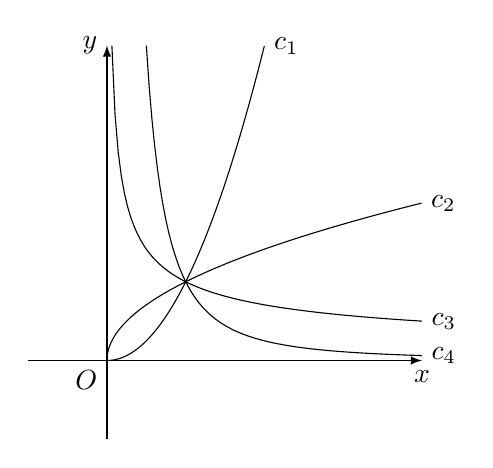
\begin{tikzpicture}[>=latex]
        \draw [->] (-1,0) -- (4,0) node [below] {$x$};
        \draw [->] (0,-1) -- (0,4) node [left] {$y$};
        \draw (0,0) node [below left] {$O$};
        \draw [domain = 0:2, samples = 100] plot (\x,\x*\x) node [right] {$c_1$};
        \draw [domain = 0:2, samples = 100] plot (\x*\x,\x) node [right] {$c_2$};
        \draw [domain = 0.0625:4, samples = 100] plot (\x, {1/sqrt(\x)}) node [right] {$c_3$};
        \draw [domain = 0.5:4, samples = 100] plot (\x, {1/\x/\x}) node [right] {$c_4$};
    \end{tikzpicture}
    \end{center}
\fourch{$-2,-\dfrac 12,\dfrac 12,2$}{$2,\dfrac 12,-\dfrac 12,-2$
}{$-\dfrac 12,-2,2,\dfrac 12$}{$2,\dfrac 12,-2,-\dfrac 12$}
\item {\tiny (002911)}已知$\alpha\in \{-2,-1,-\dfrac 12,\dfrac 12,1,2,3\}$, 若幂函数$f(x)=x^\alpha$为奇函数, 且在$(0,+\infty)$上递减, 则$\alpha=$\blank{50}.
\item {\tiny (002912)}函数$y=f(x)$满足两个条件:
\textcircled{1} $y=f(x)$是两个幂函数的和函数; \textcircled{2} $y=f(x)$的最小值为2, 则$y=f(x)$的解析式可以是\blank{50}.
\item {\tiny (002914)}设常数$m\in \mathbf{R}$. 若幂函数$y=(m^2-m-1)x^{m^2-2m-1}$在$(0,+\infty)$上是增函数, 则$m$的值为\blank{50}.
\item {\tiny (002916)}函数$y=1-(x+2)^{-2}$可以先将幂函数$y=x^{-2}$的图像向\blank{50}平移$2$个单位, 再以\blank{50}轴为对称轴作对称变换, 最后向\blank{50}平移$1$个单位.
\item {\tiny (002918)}设常数$t\in \mathbf{Z}$. 已知幂函数$y=(t^3-t+1){x^{\frac 13(1+2t-t^2)}}$是偶函数, 且在区间$(0,+\infty)$上是增函数, 求整数$t$的值, 并作出相应的幂函数的大致图像.
\item {\tiny (002921)}函数$y=-(x+1)^{-3}$的图像可以先将幂函数$y=x^{-3}$的图像向\blank{50}平移1个单位, 再以\blank{50}轴为对称轴作对称变换.
\item {\tiny (002922)}设$\alpha \in \{-3,-\dfrac 23,-\dfrac 12,-\dfrac 13,\dfrac 13,1,\dfrac 32,2\}$. 已知幂函数$y=x^{\alpha}$是奇函数, 且在区间$(0,+\infty)$上是减函数, 则满足条件的$\alpha$的值是\blank{50}.
\item {\tiny (002923)}下列关于幂函数图像及性质的叙述中, 正确的叙述的序号是\blank{50}.\\
\textcircled{1} 对于一个确定的幂函数, 第二、三象限不可能同时有该幂函数的图像上的点;\\
\textcircled{2} 若某个幂函数图像过$(-1,-1)$, 则该幂函数是奇函数;\\
\textcircled{3} 若某个幂函数在定义域上递增, 则该幂函数图像必经过原点;\\
\textcircled{4} 幂函数图像不会经过点$(-\dfrac 12,8)$以及$(-8,-4)$.
\item {\tiny (002924)}设$y=f(x)$与$y=g(x)$是两个不同的幂函数, 集合$M=\{x|f(x)=g(x)  \}$, 则集合$M$中的元素是\bracket{20}.
\fourch{$1$或$2$}{$1$或$3$}{$1$或$2$或$3$}{$1$或$2$或$3$或$4$}
\item {\tiny (002925)}已知幂函数$y=x^{\frac qp}$($p\in \mathbf{N}^*,\ q\in \mathbf{N}^*$, $p,q$互质)的图像如图所示, 则\bracket{20}.
\begin{center}
    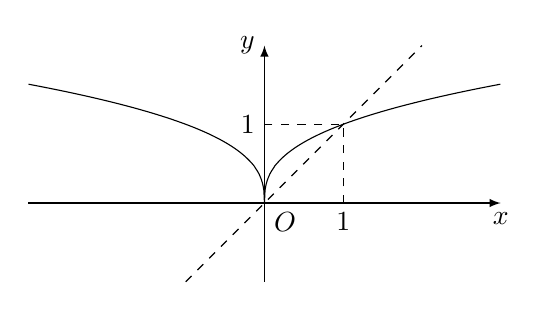
\begin{tikzpicture}[>=latex]
        \draw [->] (-3,0) -- (3,0) node [below] {$x$};
        \draw [->] (0,-1) -- (0,2) node [left] {$y$};
        \draw (0,0) node [below right] {$O$};
        \draw [dashed] (-1,-1) -- (2,2);
        \draw [domain = 0:3, samples = 400] plot (\x,{\x^(3/8)}) plot (-\x,{\x^(3/8)});
        \draw [dashed] (1,0) node [below] {$1$} -- (1,1) -- (0,1) node [left] {$1$};
    \end{tikzpicture}
\end{center}
\twoch{$p,q$均为奇数}{$p$是奇数, $q$是偶数, 且$0<\dfrac qp<1$}{$p$是偶数, $q$是奇数}{$p$是奇数, $q$是偶数, 且$\dfrac qp>1$}
\item {\tiny (002930)}函数$y=\log_2 \dfrac 1{x-1}$的反函数是\blank{50}.
\item {\tiny (002932)}函数$y=\dfrac{2^x}{{2^x}-1}$($x>0$)的反函数是\blank{50}.
\item {\tiny (002934)}记$y=f^{-1}(x)$是$y=f(x)$的反函数. 若函数$f(x)=\log_3x$, 则$f^{-1}(-\log_9 2)$=\blank{50}.
\item {\tiny (002941)}(1) 函数$y=x^2+2x-3\ (x\ge 0)$的反函数为\blank{50};\\
(2) 函数$y=\dfrac{\mathrm{e}^x-1}{{\mathrm{e}}^x+1}$的反函数为\blank{50};\\
(3) 函数$y=x|x|$的反函数为\blank{50}.
\item {\tiny (002942)}已知函数$y=f(x)$是奇函数, 且$y=g(x)$是$y=f(x)$的反函数. 若$x\ge 0$时, $f(x)=3^x-1$, 则$g(-8)$=\blank{50}.
\item {\tiny (002944)}求函数$y=\begin{cases}x^2-2x+2, & x\le 1,\\(\dfrac 12)^x, & x>1  \end{cases}$的反函数.
\item {\tiny (002945)}设常数$a>0$且$a\ne 1$. 求函数$f(x)=\log_a(x+\sqrt{x^2-1})$的反函数.
\item {\tiny (002948)}设$a>0$, 函数$f(x)=\dfrac 1{1+a\cdot 2^x}$.\\
(1) 若$a=1$, 求$f(x)$的反函数$f^{-1}(x)$;\\
(2) 求函数$y=f(x)\cdot f(-x)$的最大值(用$a$表示);\\
(3) *设$g(x)=f(x)-f(x-1)$. 若对任意$x\in (-\infty ,0]$, $g(x)\ge g(0)$恒成立, 求$a$的取值范围.
\item {\tiny (002950)}若$\log_35=a$, $\log_57=b$ , 用$a,b$表示$\log_{75}63=$\blank{50}.
\item {\tiny (002951)}若$3^a=4^b=6^c$, 且$a,b,c$都是正数, 则$\dfrac{-2ab+2bc+ac}{abc}$的值为\blank{50}.
\item {\tiny (002952)}若不等式$(a-1)^x<1$的解集为$(-\infty,0)$, 则实数$a$的取值范围是\blank{50}.
\item {\tiny (002953)}函数$f(x)=\dfrac{\sqrt{4-x^2}}{\lg |x-1|}$的定义域为\blank{50}.
\item {\tiny (002954)}为了得到函数$y=\lg\dfrac{x+3}{10}$的图像, 只需把函数$y=\lg x$的图像上所有的点\bracket{20}.
\onech{向左平移$3$个单位长度, 再向上平移$1$个单位长度}{向右平移$3$个单位长度, 再向上平移$1$个单位长度}{向左平移$3$个单位长度, 再向下平移$1$个单位长度}{向右平移$3$个单位长度, 再向下平移$1$个单位长度}
\item {\tiny (002955)}设常数$a>0,\ a\ne 1$. 函数$f(x)=a^x$在$[0,1]$上的最大值和最小值之和为$a^2$, 则$a=$\blank{50}.
\item {\tiny (002956)}若集合$A=\{y|y=2\cdot (\dfrac 13)^{|x|}\}$, $B=\{ a|\log_a(3a-1)>0\}$, 则$A\cap B$=\blank{50}.
\item {\tiny (002957)}*已知函数$f(x)=|3^x-1|$, $c<b<a$, 且$f(b)<f(a)<f(c)$, 在下列关系式中, 一定成立的关系式的序号是\blank{50}.
\textcircled{1} $3^a+3^b>2$; \textcircled{2} $3^a+3^b<2$; \textcircled{3} $3^c<1$; \textcircled{4} $3^a+3^c<2$.
\item {\tiny (002958)}已知函数$f(x)=\dfrac{3^x-3^{-x}}{3^x+3^{-x}}$.\\
(1) 证明$f(x)$在$(-\infty,+\infty)$上是增函数;\\
(2) 求$f(x)$的值域.
\item {\tiny (002959)}已知函数$y=(\log_2\dfrac x{2^a})(\log_2\dfrac x4)$, $x\in [\sqrt 2,4]$, 试求该函数的最大值$g(a)$.
\item {\tiny (002960)}已知函数$f(x)=a\cdot 2^x+b\cdot 3^x$, 其中常数$a,b$满足$ab\ne 0$.\\
(1) 若$ab>0$, 判断函数$y=f(x)$的单调性;\\
(2) 若$ab<0$, 求$f(x+1)>f(x)$时$x$的取值范围.
\item {\tiny (002961)}不等式$\log_{\frac 12}(x-1)\ge 1$的解集为\blank{50}.
\item {\tiny (002962)}设常数$a\in \mathbf{R}$. 若函数$f(x)=\dfrac 1{2^x-1}+a$为奇函数, 则$a$=\blank{50}.
\item {\tiny (002963)}若$\log_23=a$, $3^b=7$, 用$a,b$表示$\log_{3\sqrt 7}2$, 则$\log_{3\sqrt 7}2$=\blank{50}.
\item {\tiny (002964)}对于函数$y=f(x)$的定义域中的任意的$x_1,x_2$($x_1\ne x_2$), 有如下结论:\\
\textcircled{1} $f(x_1+x_2)=f(x_1)\cdot f(x_2)$; \textcircled{2} $f(x_1\cdot x_2)=f(x_1)+f(x_2)$;\\ \textcircled{3} $\dfrac{f(x_1)-f(x_2)}x_1-x_2>0$; \textcircled{4} $f(\dfrac{x_1+x_2}2)<\dfrac{f(x_1)+f(x_2)}2$. 
\\当$y=\ln x$时, 上述结论中, 正确结论的序号是\blank{50}.
\item {\tiny (002965)}(1) *函数$y=\log_a|x-b|$在$(0,+\infty)$上递增, 则$a$、$b$满足\bracket{20}.
\fourch{$a>1$且$b\ge 0$}{$a>1$且$b\le 0$}{$0<a<1$且$b\ge 0$}{$0<a<1$且$b\le 0$}
(2) 函数$f(x)=\log_a|ax^2-x| \ (a>0,\ a\ne 1)$在区间$[3,4]$上是增函数, 则实数$a$的范围是\blank{50}.
\item {\tiny (002966)}*已知常数$a>1$, 函数$y=|\log_ax|$的定义域为区间$[m,n]$, 值域为区间$[0,1]$. 若$n-m$的最小值为$\dfrac 56$, 则$a$=\blank{50}.
\item {\tiny (002967)}*设常数$a>0$ ,$a\ne 1$. 已知函数$f(x)=\log_ax$. 若对于任意$x\in [3,+\infty)$都有$|f(x)|\ge 1$成立, 则$a$的取值范围为\blank{50}.
\item {\tiny (002968)}*已知函数$f(x)=2+\log_3 x\ (3\le x\le 27)$.\\
(1) 求函数$y=f(x^2)$的定义域;\\
(2) 求函数$g(x)={[f(x)]}^2+f(x^2)$的值域.
\item {\tiny (002969)}已知定义域为$\mathbf{R}$的函数$y=f(x)$为奇函数, 且满足$f(x+2)=-f(x)$. 当$x\in [0,1]$时, $f(x)=2^x-1$.\\
(1) 求$y=f(x)$在区间$[-1,0)$上的解析式;\\
(2) 求$f(\log_{\frac 12}24)$的值.
\item {\tiny (002970)}*已知函数$f(x)=1+a\cdot (\dfrac 12)^x+(\dfrac 14)^x$.\\
(1) 当$a=1$时, 求函数$y=f(x)$在$(-\infty,0)$上的值域;\\
(2) 对于定义在集合$D$上的函数$y=f(x)$, 如果存在常数$M>0$, 满足: 对任意$x\in D$, 都有$|f(x)|\le M$成立, 则称$f(x)$是$D$上的有界函数, 其中$M$称为函数$f(x)$的一个上界.若函数$y=f(x)$在$[0,+\infty)$上是以$3$为一个上界的有界函数, 求实数$a$的取值范围.
\item {\tiny (002980)}已知函数$y=x+\dfrac ax$有如下性质: 如果常数$a>0$, 那么该函数在$(0, \sqrt a]$上是减函数, 在$[\sqrt a, +\infty)$上是增函数.\\
(1) 设常数$c\in [1,+\infty)$, 求函数$f(x)=x+\dfrac cx \ (1\le x\le 2)$的最大值和最小值;\\
(2) *设常数$c>0$. 当$n$是正整数时, 研究函数$g(x)=x^n+\dfrac c{x^n}$的单调性, 并说明理由.
\item {\tiny (002993)}函数$y=\dfrac{3^x-1}{3^x-2}$的值域是\blank{50}.
\item {\tiny (002994)}函数$y=\log_{\frac 12}(-x^2+2x+3)$的值域是\blank{50}.
\item {\tiny (003000)}已知函数$f(x)=\log_a(x+\sqrt{x^2+1}), \ a>1$.\\
(1) 求$f(x)$的定义域和值域;\\
(2) 求$f^{-1}(x)$;\\
(3) 判断$f^{-1}(x)$的奇偶性、单调性;\\
(4) 若实数$m$满足$f^{-1}(1-m)+f^{-1}(1-m^2)<0$, 求$m$的范围.
\item {\tiny (003014)}用二分法, 可以计算得方程$6-x=\lg x$的解是\blank{50}(结果精确到0.01).
\item {\tiny (003015)}方程$6-x=\log_2 x$的解集是\blank{50}.
\item {\tiny (003017)}若方程$2^x=(\dfrac 12)^{-\frac 1x+1}$的两个实数解为$x_1, x_2$, 则$x_1+x_2$=\blank{50}.
\item {\tiny (003018)}设常数$a\in \mathbf{R}$. 若关于$x$的方程$\lg^2x-\lg x^2+a-2=0$有两个不同的实数解$x_1, x_2$, 则\\
(1) $x_1\cdot x_2$=\blank{50};\\
(2) $a$的取值范围是\blank{50}.
\item {\tiny (003019)}(1) 设常数$a\in \mathbf{R}$. 若关于$x$的方程$9^x-(a+2)\cdot 3^x+4=0$有实数解, 则$a$的取值范围是\blank{50};\\
(2)设常数$a\in \mathbf{R}$.若关于$x$的方程$9^x-3^x+a=0$有两个不同的实数解$x_1, x_2$, 则$a$的取值范围是\blank{50}.
\item {\tiny (003024)}方程$4^{x+1}-13\cdot 2^x+3=0$的解集是\blank{50}.
\item {\tiny (003025)}方程$\log_2(x-1)=\log_4(2-x)$的解集是\blank{50}.
\item {\tiny (003026)}方程$2\log_2(x-1)=2+\log_2 x$的解集是\blank{50}.
\item {\tiny (003027)}方程$\log_3(3^{x-1}-3^{-1})\cdot \log_3(3^{x-2}-3^{-2})=2$的解集是\blank{50}.
\item {\tiny (003029)}方程$2(4^x+4^{-x})-3(2^x-2^{-x})-4=0$的解集是\blank{50}.
\item {\tiny (003032)}设常数$a\in \mathbf{R}$.已知函数$f(x)=4^x-a\cdot 2^x+a+3$.\\
(1) 若函数$y=f(x)$有且仅有一个零点, 求$a$的取值范围;\\
(2) 若函数$y=f(x)$有零点, 求$a$的取值范围.
\item {\tiny (003041)}已知实数$ab$满足等式$(\dfrac 12)^a=(\dfrac 13)^b$, 下列五个关系式:\\
\textcircled{1} $0<b<a$; \textcircled{2} $a<b<0$; \textcircled{3} $0<a<b$; \textcircled{4} $b<a<0$; \textcircled{5} $a=b=0$. 其中不可能成立的关系式的序号为\blank{50}.
\item {\tiny (003043)}设常数$k\in \mathbf{R}$. 已知关于x的不等式$k\cdot 4^x-2^{x+1}+6k<0$.\\
(1) 若不等式的解集为开区间$(1, \log_2 3)$, 求$k$的取值范围;\\
(2) 若不等式对一切$x\in (1,\log_2 3)$都成立, 求$k$的取值范围;\\
(3) *若不等式的解集为开区间$(1,\log_2 3)$的子集, 求$k$的取值范围;\\
(4) *若不等式在开区间$(1,\log_2 3)$内存在解, 求$k$的取值范围.
\item {\tiny (003052)}设常数$a\in \mathbf{R}$.若对于任意实数$x\in (-\infty ,-1]$, 不等式$1+2^x+(a-a^2)\cdot 4^x>0$恒成立, 求$a$的取值范围.
\item {\tiny (003601)}下列函数中, 既是奇函数又是减函数的是\bracket{20}.
\fourch{$y=-3x$}{$y=x^3$}{$y=\log_3^x$}{$y=3^x$}
\item {\tiny (003636)}已知函数$f(x)$的周期为$1$, 当$0<x\le 1$时, $f(x)=\log_2 x$, 则$f\left(\dfrac{3}{2}\right)$的值为\blank{50}.
\item {\tiny (003655)}设常数$a\in \mathbf{R}$, 函数$f(x)=\log_2(x+a)$. 若$f(x)$的反函数的图像经过点$(3,1)$, 则$a=$\blank{50}.
\item {\tiny (003658)}已知$\alpha\in \left\{-2,-1,-\dfrac{1}{2},\dfrac{1}{2},1,2,3\right\}$. 若幂函数$f(x)=x^{\alpha}$为奇函数, 且在$(0,+\infty)$上递减, 则$\alpha=$\blank{50}.
\item {\tiny (003662)}已知常数$a>0$, 函数$f(x)=\dfrac{2^x}{2^x+ax}$的图像经过点$P\left(p,\dfrac{6}{5}\right)$, $Q\left(q,-\dfrac{1}{5}\right)$. 若$2^{p+q}=36pq$, 则$a=$\blank{50}.
\item {\tiny (003680)}定义在$(0,+\infty)$上的函数$y=f(x)$的反函数为$y=f^{-1}(x)$. 若$g(x)=\begin{cases}3^x-1, & x\le 0,\\ f(x), & x>0\end{cases}$为奇函数, 则$f^{-1}(x)=2$的解为\blank{50}.
\item {\tiny (003694)}已知函数$f(x)=\log_a x+x-b$($a>0$且$a\ne 1$). 当$2<a<3<b<4$时, 函数$f(x)$的零点$x_0\in (n,n+1), \ n\in \mathbf{N}^*$, 则$n=$\blank{50}.
\item {\tiny (003709)}若函数$y=a^x+b$($a>0$且$a\ne 1$)的图像经过点$(1,7)$, 其反函数的图像经过点$(4,0)$, 则$a-b=$\blank{50}.
\item {\tiny (003718)}已知函数$f(x)=\begin{cases}
\log_2(x+4), & x\ge 0,\\f(x+1)-f(x+2), & x<0,\end{cases}$ 则$f(-3)$的值为\blank{30}.
\fourch{$1$}{$0$}{$2$}{$-2$}
\item {\tiny (003726)}若函数$f(x)=\dfrac{k-2^x}{1+k\cdot 2^x}, \ (k\ne 1, \ k\in \mathbf{R})$在定义域内为奇函数, 则$k=$\blank{50}.
\item {\tiny (003730)}下列函数中, 与函数$y=x^{2n+1} \ (n\in \mathbf{N}^*)$的值域相同的函数为\blank{30}.
\fourch{$y=\left(\dfrac 12\right)^{x+1}$}{$y=\ln(x+1)$}{$y=\dfrac{x+1}{x}$}{$y=x+\dfrac 1x$}
\item {\tiny (003746)}幂函数$f(x)$的图像经过点$(2,\sqrt{2})$, 且$f^{-1}(x)$为$f(x)$的反函数, 则$f^{-1}(4)=$\blank{50}.
\item {\tiny (003747)}若$\log_a \dfrac 23<1 \ (a>0, \ a\ne 1)$, 则实数$a$的取值范围为\blank{50}.
\item {\tiny (003757)}设函数$f(x)=x^3+\dfrac{2^x-1}{2^x+1}$, 已知$a\in (-1,1)$, $b\in (-1,1)$. 则$a+b\ge 0$是$f(a)+f(b)\ge 0$的\blank{30}.
\twoch{充分不必要条件}{必要不充分条件}{充分必要条件}{既不充分也不必要条件}
\item {\tiny (003770)}函数$f(x)=2^x+x^3-2$在区间$(0,1)$内的零点的个数是\blank{30}.
\fourch{$0$}{$1$}{$2$}{$3$}
\item {\tiny (003772)}定义在$(-\infty,0)\cup (0,+\infty)$上的函数$f(x)$, 如果对于任意给定的等比数列$\{a_n\}$, $\{f(a_n)\}$仍是等比数列, 则称$f(x)$为``保等比数列函数''. 现有定义在$(-\infty,0)\cup (0,+\infty)$上的如下函数: \textcircled{1} $f(x)=x^2$; \textcircled{2} $f(x)=2^x$; \textcircled{3} $f(x)=\sqrt{|x|}$; \textcircled{4} $f(x)=\ln|x|$. 则其中是``保等比数列函数''的$f(x)$的序号为\blank{30}.
\fourch{\textcircled{1}\textcircled{2}}{\textcircled{3}\textcircled{4}}{\textcircled{1}\textcircled{3}}{\textcircled{2}\textcircled{4}}
\item {\tiny (003775)}已知$U=\left\{y\left|y=\log_\frac 12 x, \ x\ge \dfrac 18\right.\right\}$, $A=\left\{x\left|y=\dfrac{1}{\sqrt{2-x}}\right.\right\}$, 则$\complement_U A=$\blank{50}.
\item {\tiny (003778)}已知函数$f(x)=4^x-k\cdot 2^{x+1}+4$在$[0,2]$上存在零点, 则实数$k\in$\blank{50}.
\item {\tiny (003789)}设函数$f(x)=\log_\frac 12 x$, $g(x)=f^{-1}(|x|)$.\\
(1) 求函数$g(x)$的解析式, 并画出大致图像;\\
(2) 若不等式$g(x)+g(2x)\le k$对任意$x\in \mathbf{R}$恒成立, 求实数$k$的取值范围.
\item {\tiny (003801)}下列函数中, 既是偶函数, 又是在区间$(0,+\infty)$上单调递减的函数为\blank{30}.
\fourch{$y=\lg\dfrac{1}{|x|}$}{$y=x^3$}{$y=3^{|x|}$}{$y=x^2$}
\item {\tiny (003815)}在同一坐标系中画出函数$y=\log_a x, \ y=a^x, y=x+a$的图像, 可能正确的是\blank{30}.
\fourch{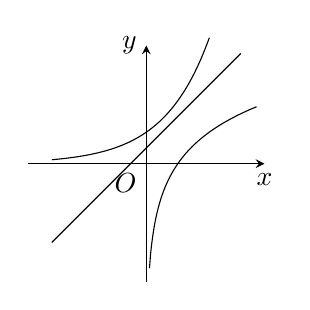
\begin{tikzpicture}[>=stealth,samples=100]
	\draw [->] (-1.5,0)--(0,0) node [below left] {$O$}--(1.5,0) node [below] {$x$};
	\draw [->] (0,-1.5)--(0,1.5) node [left] {$y$};
	\draw [domain=-3:3] plot ({\x*0.4},{(\x+0.5)*0.4});
	\draw [domain=-3:2] plot ({\x*0.4},{exp(\x*ln(2))*0.4});
	\draw [domain=0.1:3.5] plot ({\x*0.4},{ln(\x)/ln(2)*0.4});
	\end{tikzpicture}}{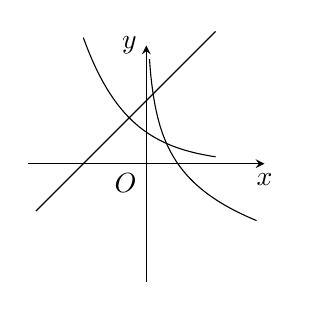
\begin{tikzpicture}[>=stealth,samples=100]
	\draw [->] (-1.5,0)--(0,0) node [below left] {$O$}--(1.5,0) node [below] {$x$};
	\draw [->] (0,-1.5)--(0,1.5) node [left] {$y$};
	\draw [domain=-3.5:2.2] plot ({\x*0.4},{(\x+2)*0.4});
	\draw [domain=-2:2.2] plot ({\x*0.4},{exp(\x*ln(1/2))*0.4});
	\draw [domain=0.1:3.5] plot ({\x*0.4},{-ln(\x)/ln(2)*0.4});
	\end{tikzpicture}}{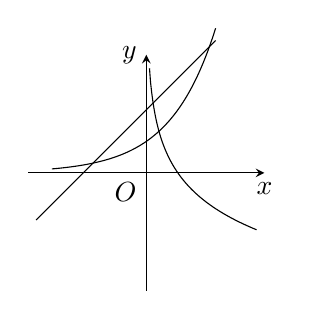
\begin{tikzpicture}[>=stealth,samples=100]
	\draw [->] (-1.5,0)--(0,0) node [below left] {$O$}--(1.5,0) node [below] {$x$};
	\draw [->] (0,-1.5)--(0,1.5) node [left] {$y$};
	\draw [domain=-3.5:2.2] plot ({\x*0.4},{(\x+2)*0.4});
	\draw [domain=-3:2.2] plot ({\x*0.4},{exp(\x*ln(2))*0.4});
	\draw [domain=0.1:3.5] plot ({\x*0.4},{-ln(\x)/ln(2)*0.4});
	\end{tikzpicture}}{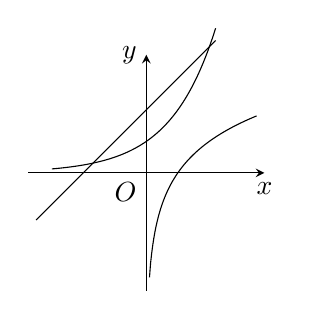
\begin{tikzpicture}[>=stealth,samples=100]
	\draw [->] (-1.5,0)--(0,0) node [below left] {$O$}--(1.5,0) node [below] {$x$};
	\draw [->] (0,-1.5)--(0,1.5) node [left] {$y$};
	\draw [domain=-3.5:2.2] plot ({\x*0.4},{(\x+2)*0.4});
	\draw [domain=-3:2.2] plot ({\x*0.4},{exp(\x*ln(2))*0.4});
	\draw [domain=0.1:3.5] plot ({\x*0.4},{ln(\x)/ln(2)*0.4});
	\end{tikzpicture}}
\item {\tiny (003828)}已知正数$x,y$满足$\ln x+\ln y=\ln (x+y)$, 则$2x+y$的最小值是\blank{50}.
\item {\tiny (003838)}已知函数$f(x)=\begin{cases}
\dfrac 3x, & x\ge 3,\\ \log_3 x, & 0<x<3,
\end{cases}$ 若关于$x$的方程$f(x)=k$有两个不同的实根, 则实数$k$的取值范围是\blank{50}.
\item {\tiny (003854)}不等式$\lg(-x)<x+1$的解集为\blank{50}.
\item {\tiny (003865)}集合$\{y|y=2^{-x}\}\cap\{y|y=\lg x, \ 0<x<100\}=$\blank{50}.
\item {\tiny (003869)}函数$f(x)=a^x+b \ (a>1, \ b<-1)$, 则$y=f^{-1}(x)$的图像一定不经过第\blank{50}象限.
\item {\tiny (003911)}已知函数$f(x)=\begin{cases}
2^x-1, & x\ge 0,\\ -x^2-2x, & x<0,
\end{cases}$ 若$f(a)=1$, 则实数$a$的值是\blank{50}.
\item {\tiny (003936)}函数$y=\ln(\cos x) \ \left(-\dfrac{\pi}{2}<x<\dfrac{\pi}{2}\right)$的大致图像是\blank{30}.
\fourch{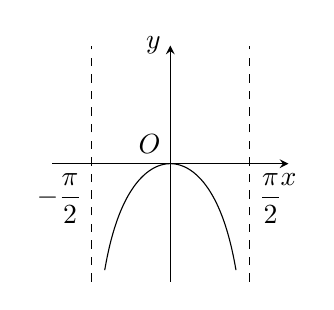
\begin{tikzpicture}[samples=200,>=stealth]
	\draw [->](-1.5,0)--(0,0) node [above left] {$O$}--(1.5,0) node [below] {$x$};
	\draw [->](0,-1.5)--(0,1.5) node [left] {$y$};
	\draw [dashed] (-1,-1.5)--(-1,1.5) (1,-1.5)--(1,1.5);
	\draw (-1,0) node [below left] {$-\dfrac{\pi}{2}$};
	\draw (1,0) node  [below right] {$\dfrac{\pi}{2}$};
	\draw [domain=-75:75] plot ({\x/90},{ln(cos(\x))});
	\end{tikzpicture}}{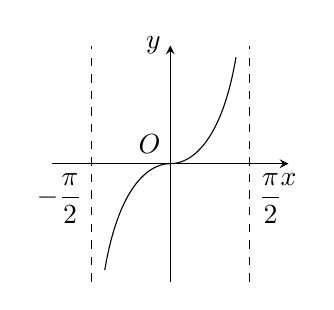
\begin{tikzpicture}[samples=200,>=stealth]
	\draw [->](-1.5,0)--(0,0) node [above left] {$O$}--(1.5,0) node [below] {$x$};
	\draw [->](0,-1.5)--(0,1.5) node [left] {$y$};
	\draw [dashed] (-1,-1.5)--(-1,1.5) (1,-1.5)--(1,1.5);
	\draw (-1,0) node [below left] {$-\dfrac{\pi}{2}$};
	\draw (1,0) node  [below right] {$\dfrac{\pi}{2}$};
	\draw [domain=-75:0] plot ({\x/90},{ln(cos(\x))});
	\draw [domain=0:75] plot ({\x/90},{-ln(cos(\x))});
	\end{tikzpicture}}{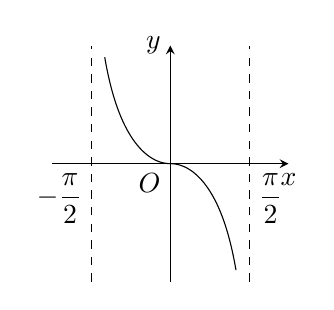
\begin{tikzpicture}[samples=200,>=stealth]
	\draw [->](-1.5,0)--(0,0) node [below left] {$O$}--(1.5,0) node [below] {$x$};
	\draw [->](0,-1.5)--(0,1.5) node [left] {$y$};
	\draw [dashed] (-1,-1.5)--(-1,1.5) (1,-1.5)--(1,1.5);
	\draw (-1,0) node [below left] {$-\dfrac{\pi}{2}$};
	\draw (1,0) node  [below right] {$\dfrac{\pi}{2}$};
	\draw [domain=-75:0] plot ({\x/90},{-ln(cos(\x))});
	\draw [domain=0:75] plot ({\x/90},{ln(cos(\x))});
	\end{tikzpicture}}{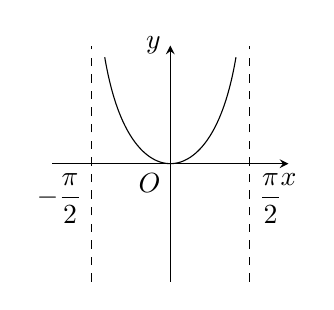
\begin{tikzpicture}[samples=200,>=stealth]
	\draw [->](-1.5,0)--(0,0) node [below left] {$O$}--(1.5,0) node [below] {$x$};
	\draw [->](0,-1.5)--(0,1.5) node [left] {$y$};
	\draw [dashed] (-1,-1.5)--(-1,1.5) (1,-1.5)--(1,1.5);
	\draw (-1,0) node [below left] {$-\dfrac{\pi}{2}$};
	\draw (1,0) node  [below right] {$\dfrac{\pi}{2}$};
	\draw [domain=-75:75] plot ({\x/90},{-ln(cos(\x))});
	\end{tikzpicture}}
\item {\tiny (003953)}已知集合$M$是满足下列性质的函数$f(x)$的全体, 存在非零常数$T$, 对任意$x\in \mathbf{R}$, 有$f(x+T)=Tf(x)$成立.\\
(1) 函数$f(x)=x$是否属于集合$M$? 说明理由;\\
(2) 设$f(x)\in M$, 且$T=2$, 已知当$1<x<2$时, $f(x)=x+\ln x$, 求当$-3<x<-2$时, $f(x)$的解析式.
\item {\tiny (004001)}已知$f(x)=\sqrt{x}$, $g(x)=kx^x$.\\
(1) 求曲线$y=f(x)$在点$(4,2)$处的切线方程;\\
(2) 若曲线$y=g(x)$经过点$(4,2)$, 求它与(1)中切线的另一个交点.
\item {\tiny (004003)}已知$f(x)=lnx$, $g(x)=\mathrm{e}^x$, 计算下列函数$y=h(x)$在点$x=1$处的导数值:\\
(1) $h(x)=3f(x)-5g(x)$;\\
(2) $h(x)=f(x)g(x)$;\\
(3) $h(x)=\dfrac{f(x)}{g(x)}$;\\
(4) $h(x)=f(2x+1)+g(3x-1)$.
\item {\tiny (004067)}已知定义在$\mathbf{R}$上的函数$f(x)$满足: \textcircled{1} $f(x)+f(2-x)=0$; \textcircled{2} $f(x)-f(-2-x)=0$; \textcircled{3} 在$[-1,1]$上表达式为$f(x)=\begin{cases} \sqrt{1-x^2}, & x\in [-1,0], \\ 1-x, & x\in (0,1], \end{cases}$ 则函数$f(x)$与$g(x)=\begin{cases} {2^x}, & x\le 0 \\ \log_\frac 12x, & x>0 \end{cases}$的图像在区间$[-3,3]$上的交点的个数为\blank{50}.
\item {\tiny (004079)}已知函数$f(x)=\log_2x$.\\
(1) 若$f(x)$的反函数是$f^{-1}(x)$, 解方程: $f^{-1}(2x+1)=3f^{-1}(x)-1$;\\
(2) 当$x\in (3m, 3m+3]$($m\in \mathbf{N}$)时, 定义$g(x)=f(x-3m)$. 设$a_n=n\cdot g(n)$, 数列$\{a_n\}$ 的前$n$项和为$S_n$, 求$a_1$、$a_2$、$a_3$、$a_4$和$S_{3n}$;\\
(3) 对于任意$a$、$b$、$c\in [M,+\infty)$, 且$a\ge b\ge c$. 当$a$、$b$、$c$能作为一个三角形的三边长时, $f(a)$、$f(b)$、$f(c)$也总能作为某个三角形的三边长, 试探究$M$的最小值.
\item {\tiny (004086)}已知函数$f(x)=\begin{cases} 2^x, & x\le 0 \\  \log_2x, & 0<x\le 1 \end{cases}$的反函数是$f^{-1}(x)$, 则$f^{-1}(\dfrac 12)=$\blank{50}.
\item {\tiny (004089)}$[x]$是不超过$x$的最大整数, 则方程$(2^x)^2-\dfrac 74\cdot [2^x]-\dfrac 14=0$满足$x<1$的所有实数解是\blank{50}.
\item {\tiny (004097)}已知函数$f(x)=1-\dfrac 6{a^{x+1}+a}$($a>0$, $a\ne 1$)是定义在$\mathbf{R}$上的奇函数.\\
(1) 求实数$a$的值及函数$f(x)$的值域;\\
(2) 若不等式 $t\cdot f(x)\ge 3^x-3$在$x\in [1,2]$上恒成立, 求实数$t$的取值范围.
\item {\tiny (004106)}方程$\log_5(4^x-11)-1=\log_5(2^x-3)$的解为$x=$\blank{50}.
\item {\tiny (004116)}已知集合$M=\{(x,y)|y=f(x)\}$, 若对于任意$(x_1,y_1)\in M$, 存在$(x_2,y_2)\in M$, 使得$x_1x_2+y_1y_2=0$成立, 则称集合$M$是``$\Omega$集合''. 给出下列$4$个集合:
\textcircled{1} $M=\{(x,y) |y=\dfrac 1x \}$; \textcircled{2} $M=\{(x,y)|y=\mathrm{e}^x-2\}$; \textcircled{3} $M=\{(x,y)|y=\cos x\}$; \textcircled{4} $M=\{(x,y)|y=\ln x\}$.
其中所有``$\Omega$集合''的序号是\bracket{20}.
\fourch{\textcircled{2}\textcircled{3}}{\textcircled{3}\textcircled{4}}{\textcircled{1}\textcircled{2}\textcircled{4}}{\textcircled{1}\textcircled{3}\textcircled{4}}
\item {\tiny (004139)}已知常数$a\in \mathbf{R}^+$, 函数$f(x)=3^x+a^2\cdot 3^{-x}$.\\
(1) 若$a=\sqrt{3}$, 解关于$x$的不等式$f(x)<4$;\\
(2) 若$f(x)$在$[3,+\infty)$上为增函数, 求$a$的取值范围.
\item {\tiny (004143)}方程$\log_3(2x+1)=2$的解是\blank{50}.
\item {\tiny (004149)}若函数$f(x)=2^x(x+a)-1$在区间$[0,1]$上有零点, 则实数$a$的取值范围是\blank{50}.
\item {\tiny (004151)}设不等式组$\begin{cases} x+y-6\ge 0, \\ x-y+2\ge 0, \\ x-3y+6\le 0 \end{cases}$表示的可行域为$\Omega$, 若指数函数$y=a^x$的图像与$\Omega$有公共点, 则$a$的取值范围是\blank{50}.
\item {\tiny (004165)}已知函数$f(x)=\log_3(\dfrac 4{x+2})$ , 则方程$f^{-1}(x)=4$的解$x=$\blank{50}.
\item {\tiny (004184)}设$m$为给定的实常数, 若函数$y=f(x)$在其定义域内存在实数$x_0$, 使得$f(x_0+m)=f(x_0)+f(m)$成立, 则称函数$f(x)$为``$G(m)$函数''.\\
(1) 若函数$f(x)=2^x$为``$G(2)$函数'', 求实数$x_0$的值;\\
(2) 若函数$f(x)=\lg \dfrac a{x^2+1}$为``$G(1)$函数'', 求实数$a$的取值范围;\\
(3) 已知$f(x)=x+b$($b\in \mathbf{R}$)为``$G(0)$函数'', 设$g(x)=x|x-4|$. 若对任意的$x_1,x_2\in[0,t]$, 当$x_1\ne x_2$时, 都有$\dfrac{g(x_1)-g(x_2)}{f(x_1)-f(x_2)}>2$成立, 求实数$t$的最大值.
\item {\tiny (004203)}已知函数$f(x)=ax+\log_2(2^x+1)$, 其中$a\in \mathbf{R}$.\\
(1) 根据$a$的不同取值, 讨论$f(x)$的奇偶性, 并说明理由;\\
(2) 已知$a>0$, 函数$f(x)$的反函数为$f^{-1}(x)$, 若函数$y=f(x)+f^{-1}(x)$在区间$[1,2]$上的最小值为$1+\log_23$, 求函数$f(x)$在区间$[1,2]$上的最大值.
\item {\tiny (004220)}已知函数\textcircled{1} $f(x)=3\ln x$; \textcircled{2} $f(x)=3\mathrm{e}^{\cos x}$; \textcircled{3} $f(x)=3\mathrm{e}^x$; \textcircled{4} $f(x)=3\cos x$; 其中对于$f(x)$定义域内的任意一个自变量$x_1$都存在唯一一个自变量$x_2$, 使$\sqrt{f(x_1)f(x_2)}=3$成立的函数是\bracket{20}.
\fourch{\textcircled{3}}{\textcircled{2}\textcircled{3}}{\textcircled{1}\textcircled{2}\textcircled{4}}{\textcircled{4}}
\item {\tiny (004229)}函数$y=2^x$($x\ge 2$)的反函数是\blank{50}.
\item {\tiny (004238)}对实数$x\in \mathbf{R}$, 函数$f(x)$满足: $f(x+1)=\sqrt{f(x)-{f^2}(x)}+\dfrac 12$, $a_n=f^2(n)-f(n)$,
数列$\{a_n\}$的前$15$项和为$-\dfrac{31}{16}$, 数列$\{c_n\}$满足$c_n+c_{n+1}=[f(2019)]^n$, 若数列$\{c_n\}$的前$n$项和$S_n$的极限存在, 则$c_1=$\blank{50}.
\item {\tiny (004256)}设$f(x)$是定义在$\mathbf{R}$上的奇函数, 当$x>0$时, $f(x)=a^x+b$($0<a<1$, $b\in \mathbf{R}$), 若$f(x)$存在反函数, 则b的取值范围是\blank{50}.
\item {\tiny (004272)}已知函数$g(x)$的图像与函数$f(x)=\log_2(3^x-1)$的图像关于直线$y=x$对称,则$g(3)=$\blank{50}.
\item {\tiny (004276)}若函数$f(x)=\log_2(2^x+1)+kx$是偶函数, 则$k=$\blank{50}.
\item {\tiny (004284)}已知函数$f(x)=m\cdot 2^x+x^2+nx$, 记集合$A=\{x|f(x)=0, \ x\in \mathbf{R}\}$, 集合$B=\{x|f(f(x))=0, \ x\in \mathbf{R}\}$.
若$A=B$, 且$A$、$B$都不是空集, 则$m+n$的取值范围是\bracket{20}.
\fourch{$[0,4)$}{$[-1,4)$}{$[-3,5]$}{$[0,7)$}
\item {\tiny (004286)}已知函数$f(x)=a-\dfrac 4{3^x+1}$($a$为实常数).\\
(1) 讨论函数$f(x)$的奇偶性, 并说明理由;\\ 
(2) 当$f(x)$为奇函数时, 对任意的$x\in [1,5]$, 不等式$f(x)\ge \dfrac u{3^x}$恒成立, 求实数$u$的最大值.
\item {\tiny (004291)}函数$y=\lg x$的反函数是\blank{50}.
\item {\tiny (004316)}方程$\log_3\dfrac 1{2^x+4}+\log_3(4^x-2)=0$的解$x=$\blank{50}.
\item {\tiny (004332)}函数$y=\log_2(x-2)$的定义域为\blank{50}.
\item {\tiny (004335)}幂函数$y=x^k$的图像经过点$(4,\dfrac 12)$, 则它的单调减区间为\blank{50}.
\item {\tiny (004355)}若函数$f(x)=2^x-3$, 则$f^{-1}(1)=$\blank{50}.
\item {\tiny (004370)}已知常数$a\in \mathbf{R}^+$, 函数$f(x)=3^x+a^2\cdot 3^{-x}$.\\
(1) 若$a=\sqrt 3$, 解关于$x$的不等式$f(x)<4$;\\
(2) 若$f(x)$在$[3,+\infty)$上为增函数, 求$a$的取值范围.
\item {\tiny (004376)}设函数$f(x)=\lg (x+1)$的反函数为$f^{-1}(x)$, 则$f^{-1}(1)=$\blank{50}.
\item {\tiny (004379)}关于$x$的方程$\log_2 x+\log_2(x-3)=2$的解为\blank{50}.
\item {\tiny (004381)}已知常数$a\in \mathbf{R}$, 函数$f(x)=a\cdot 4^x+2^x+1$在$[3,+\infty)$上单调递减, 则$a$的取值范围为\blank{50}.
\item {\tiny (004386)}已知常数$a\in \mathbf{R}$, 函数$f(x)=ax^2+\lg \dfrac{1+x}{1-x}$.\\
(1) 若$a=0$, 判断$f(x)$的单调性并证明;\\
(2) 问: 是否存在$a$, 使得$f(x)$为奇函数? 若存在, 求出所有$a$的值; 若不存在, 说明理由.
\item {\tiny (004387)}设函数$f(x)$的定义域为$(0,+\infty)$, 若对任意$x\in (0,+\infty)$, 恒有$f(2x)=2f(x)$, 则称$f(x)$为``$2$阶缩放函数''.\\
(1) 已知函数$f(x)$为``$2$阶缩放函数'', 当$x\in (1,2]$时, $f(x)=1-\log_2 x$, 求$f(2\sqrt{2})$的值;\\
(2) 已知函数$f(x)$为``$2$阶缩放函数'', 当$x\in (1,2]$时, $f(x)=\sqrt{2x-x^2}$, 求证: 函数$y=f(x)-x$在$(1,+\infty)$上无零点.
\item {\tiny (004390)}已知函数$f(x)$的反函数$f^{-1}(x)=\log_2x$, 则$f(-1)=$\blank{50}.
\item {\tiny (004395)}$f(x)$是偶函数, 当$x\ge 0$时, $f(x)=2^x-1$, 则不等式$f(x)>1$的解集为\blank{50}.
\item {\tiny (004396)}方程$1+\log_2x=\log_2(x^2-3)$的解为\blank{50}.
\item {\tiny (004397)}已知函数$f(x)=\begin{cases}  x^2+(4a-3)x+3a,& x<0, \\ \log_a(x+1)+1,& x\ge 0, \end{cases}$($a>0$, $a\ne 1$)在$\mathbf{R}$上单调递减, 且关于$x$的方程$|f(x)|=2-x$恰好有两个不相等的实数解, 则$a$的取值范围是\blank{50}.
\item {\tiny (004401)}下列函数中, 值域为$(0,+\infty)$的是\bracket{20}.
\fourch{$y=x^2$}{$y=\dfrac 2x$}{$y=2^x$}{$y=|\log_2x|$}
\item {\tiny (004403)}设集合$A=\{y|y=a^x,\ x>0\}$(其中常数$a>0,  \ a\ne 1$), $B=\{y|y=x^k,\ x\in A\}$(其中常数$k\in \mathbf{Q}$), 则``$k<0$''是``$A\cap B=\varnothing$''的\bracket{20}.
\twoch{充分非必要条件}{必要非充分条件}{充分必要条件}{既非充分又非必要条件}
\item {\tiny (004408)}记函数$f(x)$的定义域为$D$. 如果存在实数$a$、$b$使得$f(a-x)+f(a+x)=b$对任意满足$a-x\in D$且$a+x\in D$的$x$恒成立, 则称$f(x)$为$\Psi$函数.\\
(1) 设函数$f(x)=\dfrac 1x-1$, 试判断$f(x)$是否为$\Psi$函数, 若是求出$a,b$, 若不是请说明理由;\\
(2) 设函数$g(x)=\dfrac 1{2^x+t}$, 其中常数$t\ne 0$, 证明: $g(x)$是$\Psi$函数;\\
(3) 若$h(x)$是定义在$\mathbf{R}$上的$\Psi$函数, 且函数$h(x)$的图像关于直线$x=m$($m$为常数)对称, 试判断$h(x)$是否为周期函数? 并证明你的结论.
\item {\tiny (004411)}若函数$y=\log_2(x-m)+1$的反函数的图像经过点$(1,3)$, 则实数$m=$\blank{50}.
\item {\tiny (004413)}已知函数$f(x)$的周期为$2$, 且当$0<x\le 1$时, $f(x)=\log_4x$, 那么$f(\dfrac 92)=$\blank{50}
\item {\tiny (004425)}函数$y=\log_2(4-x^2)$的定义域是\blank{50}.
\item {\tiny (004429)}已知函数$f(x)=a\cdot 2^x+3-a$($a\in \mathbf{R}$且$a\ne 0$)的反函数为$y=f^{-1}(x)$, 则函数$y=f^{-1}(x)$的图像经过的定点的坐标为\blank{50}.
\item {\tiny (004435)}集合$A=\{y|y=\log_{\frac 12}x-x,1\le x\le 2\}$, $B=\{x|x^2-5tx+1\le 0\}$, 若$A\cap B=A$, 则实数$t$的取值范围是\blank{50}.
\item {\tiny (004440)}已知函数$f(x)=\begin{cases}\log_{\frac 12}(1-x), & -1\le x\le n,  \\ 2^{2-|x-1|}-3, & n<x\le m,  \end{cases}$($n<m$)的值域是$[-1,1]$, 有下列结论:
\textcircled{1} 当$n=0$时, $m$的取值范围为$(0,2]$; \textcircled{2}  当$n=\dfrac 12$时, $m$的取值范围为$(\dfrac 12,2]$; \textcircled{3}  当$n\in [0,\dfrac 12)$时, $m$的取值范围为$[1,2]$; \textcircled{4}  当$n\in [0,\dfrac 12)$时, $m$的取值范围为$(n,2]$;
其中结论正确的所有的序号是\bracket{20}.
\fourch{\textcircled{1}\textcircled{2}}{\textcircled{3}\textcircled{4}}{\textcircled{2}\textcircled{3}}{\textcircled{2}\textcircled{4}}
\item {\tiny (004444)}定义区间$(m,n)$、$[m,n]$、$(m,n]$、$[m,n)$的长度均为$n-m$, 已知不等式$\dfrac 7{6-x}\ge 1$的解集为$A$.\\
(1) 求$A$的长度;\\
(2) 函数$f(x)=\dfrac{(a^2+a)x-1}{a^2x}$($a\in \mathbf{R}$, $a\ne 0$)的定义域与值域都是$[m,n]$($n>m$), 求区间$[m,n]$的最大长度;\\
(3) 关于$x$的不等式$\log_2x+\log_2(tx+3t)<2$的解集为$B$, 若$A\cap B$的长度为$6$, 求实数$t$的取值范围.
\item {\tiny (004445)}对于函数$y=f(x)$($x\in D$), 如果存在实数$a$、$b$($a\ne 0$, 且$a=1$, $b=0$不同时成立), 使得$f(x)=f(ax+b)$对$x\in D$恒成立, 则称函数$f(x)$为``$(a,b)$映像函数''.\\
(1) 判断函数$f(x)=x^2-2$是否是``$(a,b)$映像函数'', 如果是, 请求出相应的$a$、$b$的值, 若不是, 请说明理由;\\
(2) 已知函数$y=f(x)$是定义在$[0,+\infty)$上的``$(2,1)$映像函数'', 且当$x\in [0,1)$时, $f(x)=2^x$, 求函数$y=f(x)$($x\in [3,7)$)的反函数;\\
(3) 在(2)的条件下, 试构造一个数列$\{a_n\}$, 使得当$x\in [a_n,{a_{n+1}})$($n\in \mathbf{N}^*$)时, $2x+1$的取值范围为$[{a_{n+1}},{a_{n+2}})$, 并求$x\in [a_n,{a_{n+1}})$($n\in \mathbf{N}^*$)时, 函数$y=f(x)$的解析式, 及$y=f(x)$($x\in [0,+\infty)$)的值域.
\item {\tiny (004447)}方程$\lg(2x+3)=2\lg x$的解为\blank{50}.
\item {\tiny (004452)}已知幂函数$y=f(x)$的图像经过点$P(4,2)$, 则它的反函数为$f^{-1}(x)=$\blank{50}.
\item {\tiny (004464)}已知$a$是实常数, 函数$f(x)=a\lg(1-x)-\lg (1+x)$.\\
(1) 若$a=1$, 求证: 函数$y=f(x)$是减函数;\\
(2) 讨论函数$f(x)$的奇偶性, 并说明理由.
\item {\tiny (004496)}已知函数$y=f(x)$存在反函数$y=f^{-1}(x)$, 若函数$y=f(x)+2^x$的图像经过点$(1,4)$, 则函数$y=f^{-1}(x)+\log_2x$的图像必过点\blank{50}.
\item {\tiny (004500)}对于定义域为$D$的函数$f(x)$, 若存在$x_1,x_2\in D$且$x_1\ne x_2$, 使得$f(x_1^2)=f(x_2^2)=2f(x_1+x_2)$, 则称函数$f(x)$具有性质$M$. 若函数$g(x)=|\log_2x-1|$, $x\in (0,a]$具有性质$M$, 则实数$a$的最小值为\blank{50}.
\item {\tiny (004509)}若存在常数$k$($k>0$), 使得对定义域$D$内的任意$x_1$、$x_2$($x_1\ne x_2$), 都有$|f(x_1)-f(x_2)|\le k|x_1-x_2|$成立, 则称函数$f(x)$在其定义域$D$是``$k-$利普希兹条件函数''.\\
(1) 若函数$f(x)=\sqrt x$($1\le x\le 4$)是``$k-$利普希兹条件函数'', 求常数$k$的取值范围;\\
(2) 判断函数$f(x)=\log_2x$是否是``$2-$利普希兹条件函数'', 若是, 请证明, 若不是, 请说明理由;\\
(3) 若$y=f(x)$($x\in \mathbf{R}$)是周期为2的``$1-$利普希兹条件函数'', 证明: 对任意的实数$x_1$、$x_2$, 都有$|f(x_1)-f(x_2)|\le 1$.
\item {\tiny (004516)}函数$f(x)=1+\log_2x$($x\ge 4$)的反函数的定义域为\blank{50}.
\item {\tiny (004530)}已知函数$f(x)$的定义域是$D$, 若对于任意的$x_1,x_2\in D$, 当$x_1<x_2$时, 都有$f(x_1)\le f(x_2)$, 则称函数$f(x)$在$D$上为``非减函数''.\\
(1) 判断$f_1(x)=x^2-4x, \ x\in [1,4]$与$f_2(x)=|x-1|+|x-2|, \ x\in [1,4]$是否是``非减函数''?\\
(2) 已知函数$g(x)=2^x+\dfrac a{2^{x-1}}$在$[2,4]$上为``非减函数'', 求实数$a$的取值范围;\\
(3) 已知函数$h(x)$在$[0,1]$上为``非减函数'', 且满足条件:
\textcircled{1}  $h(0)=0$; \textcircled{2}  $h(\dfrac x3)=\dfrac 12h(x)$; \textcircled{3}  $h(1-x)=1-h(x)$, 求 $h(\dfrac 1{2020})$的值.
\item {\tiny (004540)}已知$y=f(x)$是定义在$\mathbf{R}$上的奇函数, 且当$x\ge 0$时, $f(x)=-\dfrac 1{4^x}+\dfrac 1{2^x}$, 则此函数的值域为\blank{50}.
\item {\tiny (004542)}已知$p$是实数, 函数$f(x)=10^x$. 若存在实数$m,n$, 使得$f(m+n)=f(m)+f(n)$与$f(m+n+p)=f(m)+f(n)+f(p)$均成立, 则$p$的最大值等于\blank{50}.
\item {\tiny (004563)}下列函数中, 值域为$[0,+\infty)$的是\bracket{20}.
\fourch{$y=2^x$}{$y=x^\frac 12$}{$y=\tan x$}{$y=\cos x$}
\item {\tiny (004569)}改革开放$40$年, 我国卫生事业取得巨大成就, 卫生总费用增长了数十倍. 卫生总费用包括个人现在支出、社会支出、政府支出, 如表为$2012$年至$2015$年我国卫生费用中个人现金支出、社会支出和政府支出的费用(单位:亿元)和在卫生总费用中的占比. 
\begin{center}
    \begin{tabular}{|p{.05\textwidth}<\centering|p{.1\textwidth}<\centering|p{.1\textwidth}<\centering|p{.1\textwidth}<\centering|p{.1\textwidth}<\centering|p{.1\textwidth}<\centering|p{.1\textwidth}<\centering|p{.1\textwidth}<\centering|}
        \hline
         & & \multicolumn{2}{c|}{个人现金卫生支出} & \multicolumn{2}{c|}{社会卫生支出} & \multicolumn{2}{c|}{政府卫生支出} \\ \hline
         年份& 卫生总费用(亿元)& 绝对数(亿元) & 占卫生总费用比重($\%$) & 绝对数(亿元) & 占卫生总费用比重($\%$)& 绝对数(亿元) & 占卫生总费用比重($\%$)\\ \hline
        $2012$ & $28119.00$ & $9656.32$ & $34.34$ & $10030.70$ & $35.67$ & $8431.98$ & $29.99$ \\ \hline
        $2013$ & $31668.95$ & $10729.34$ & $33.88$ & $11393.79$ & $35.98$ & $9545.81$ & $30.14$ \\ \hline
        $2014$ & $35312.40$ & $11295.41$ & $31.99$ & $13437.75$ & $38.05$ & $10579.23$ & $29.96$ \\ \hline
        $2015$ & $40974.64$ & $11992.65$ & $29.27$ & $16506.71$ & $40.29$ & $12475.28$ & $30.45$ \\ \hline
    \end{tabular}
\end{center}
(数据来源于国家统计年鉴)\\
(1) 指出$2012$年到$2015$年之间我国卫生总费用中个人现金支出占比和社会支出占比的变化趋势;\\
(2) 设$t=1$表示$1978$年, 第$t$年卫生总费用与年份$t$之间拟合函数$f(t)=\dfrac{357876.6053}{1+\mathrm{e}^{6.4420-0.1136t}}$, 研究函数$f(t)$的单调性, 并预测我国卫生总费用首次超过$12$万亿的年份.
\item {\tiny (004620)}已知函数$f(x)=\lg (x+1)$的反函数为$y=f^{-1}(x)$, 则$f^{-1}(2)=$\blank{50}.
\item {\tiny (004640)}方程$2^x=3$的解为$x=$\blank{50}.
\item {\tiny (004649)}已知$f(x)=m(x-2m)(x+m+3)$, $g(x)=2^x-2$, 满足对于任意的$x\in \mathbf{R}$, $f(x)<0$或$g(x)<0$, 则$m$的取值范围是\blank{50}.
\item {\tiny (004665)}方程$\lg (x+2)=2\lg x$的解为\blank{50}.
\item {\tiny (004671)}设$f(x)$是定义在$\mathbf{R}$上的函数, 且满足$f(1)=0$.若$y=f(x)+a\cdot 2^x$是奇函数, $y=f(x)+3^x$是偶函数, 则$a$的值为\blank{50}.
\item {\tiny (004680)}已知函数$f(x)=2^x+\dfrac a{2^x}$, $a$为实常数.\\
(1) 若函数$f(x)$为奇函数, 求$a$的值;\\
(2) 若$x\in [0,1]$时$f(x)$的最小值为$2$, 求$a$的值;\\
(3) 若方程$f(x)=6$有两个不等的实根$x_1,x_2$, 且$|x_1-x_2|\le 1$, 求$a$的取值范围.
\item {\tiny (004689)}方程$\log_3(x^2-1)=2+\log_3(x-1)$的解为$x=$\blank{50}.
\item {\tiny (004704)}函数$y=\log_2(x+1)$的反函数为\blank{50}.
\item {\tiny (004729)}函数$f(x)=1+\lg x$的反函数是$f^{-1}(x)$=\blank{50}.
\item {\tiny (004731)}已知集合$A=\{-2,-1,-\dfrac 12,\dfrac 13,\dfrac 12,1,2,3\}$, 从集合$A$中任取一个元素$a$, 使函数$y=x^a$是奇函数且在$(0,+\infty)$上递增的概率为\blank{50}.
\item {\tiny (004757)}下列函数中既是奇函数, 又在区间$(0,+\infty)$上单调递减的函数为\bracket{20}.
\fourch{$y=\sqrt x$}{$y=\log_{\frac 12}x$}{$y=-x^3$}{$y=x+\dfrac 1x$}
\item {\tiny (004760)}已知以下三个陈述句:\\
$p$: 存在$a\in \mathbf{R}$且$a\ne 0$, 对任意的$x\in \mathbf{R}$, 均有$f(2^{x+a})<f(2^x)+f(a)$恒成立;\\
$q_1$: 函数$y=f(x)$是定义域为$\mathbf{R}$的减函数, 且对任意的$x\in \mathbf{R}$, 都有$f(x)>0$;\\
$q_2$: 函数$y=f(x)$是定义域为$\mathbf{R}$的增函数, 存在$x_0<0$, 使得$f(x_0)=0$;\\
用这三个陈述句组成两个命题, 命题$S$: ``若$q_1$, 则$p$''; 命题$T$: ``若$q_2$, 则$p$''. 关于$S,T$以下说法正确的是\bracket{20}.
\twoch{只有命题$S$是真命题}{只有命题$T$是真命题}{两个命题$S,T$都是真命题}{两个命题$S,T$都不是真命题}
\item {\tiny (004902)}若$a=\log_{0.2}0.3$, $b=\log_{0.3}0.2$, $c=1$, 则$a,b,c$的大小关系是\bracket{20}.
\fourch{$a>b>c$}{$b>a>c$}{$b>c>a$}{$c>b>a$}
\item {\tiny (004907)}若$x>y>1$, $0<a<1$, 则下列各式中正确的一个是\bracket{20}.
\fourch{${x^{-a}}>{y^{-a}}$}{$(\sin a)^x>(\sin a)^y$}{$\log_{\frac 1a}x<\log_{\frac 1a}y$}{$1+a^{x+y}>a^x+a^y$}
\item {\tiny (004909)}设$a>0$, $a\ne 1$, $t>0$, 比较$\dfrac 12\log_at$和$\log_a\dfrac{t+1}2$的大小.
\item {\tiny (004975)}设$a,b\in \mathbf{R}^+$, 且$a\ne b$, 求证: $a^ab^b>a^bb^a$.
\item {\tiny (004981)}已知$-1\le x\le 1$, $n\ge 2$, $n\in \mathbf{N}$, 求证: $(1-x)^n+(1+x)^n\le 2^n$.
\item {\tiny (005008)}下列各式中, 对任何实数$x$都成立的一个是\bracket{20}.
\fourch{$\lg (x^2+1)\ge \lg 2x$}{$x^2+1>2x$}{$\dfrac 1{x^2+1}\le 1$}{. $x+\dfrac 1x\ge 2$}
\item {\tiny (005012)}若$a>1$, $b>1$, $c>1$, 则$\log_ab+\log_ba$的最小值为\blank{50}, $\log_ab+\log_bc+\log_ca$的最小值为\blank{50}.
\item {\tiny (005013)}若$0<a<1$, $0<b<1$, 则$\log_ab+\log_ba$的最小值为\blank{50}.
\item {\tiny (005014)}若$a>1$, $0<b<1$, 则$\log_ab+\log_ba$的最大值为\blank{50}.
\item {\tiny (005016)}若$a,b,c$均大于1, 且$\log_ac\cdot \log_bc=4$, 则下列各式中, 一定正确的是\bracket{20}.
\fourch{$ac\ge b$}{$ab\ge c$}{$bc\ge a$}{$ab\le c$}
\item {\tiny (005023)}利用公式$a^2+b^2\ge 2ab$或$a+b\ge 2\sqrt{ab}$($a,b\ge 0$), 求证: $\log_{0.5}(\dfrac 1{4^a}+\dfrac 1{4^b})\le a+b-1$.
\item {\tiny (005036)}利用$a^2+b^2+c^2\ge ab+bc+ca(a,b,c\in \mathbf{R})$, 证明: 若$a,b,c>0$, $n\in \mathbf{N}$, $f(n)=\lg \dfrac{a^n+b^n+c^n}3$, 则$2f(n)\le f(2n)$.
\item {\tiny (005038)}利用放缩法并结合公式$ab\le (\dfrac{a+b}2)^2$, 证明: $\log_a(a-1)\cdot \log_a(a+1)<1$($a>1$).
\item {\tiny (005085)}已知$f(x)=\lg \dfrac{1+2^x+a\cdot 4^x}3$($a\in \mathbf{R}$).\\
(1) 如果$x\le 1$时$f(x)$有意义, 求$a$的取值范围;\\
(2) 如果$0<a\le 1$, 求证: $x\ne 0$时, $2f(x)<f(2x)$.
\item {\tiny (005103)}下列函数中, 最小值为$2$的是\bracket{20}.
\twoch{$x+\dfrac 1x$}{$\dfrac{x^2+2}{\sqrt{x^2+1}}$}{$\log_ax+\log_xa$($a>0$, $x>0$, $a\ne 1$, $x\ne 1$)}{$3^x+3^{-x}$($x>0$)}
\item {\tiny (005104)}若$\log_{\sqrt 2}x+\log_{\sqrt 2}y=4$, 则$x+y$的最小值是\bracket{20}.
\fourch{$8$}{$4\sqrt 2$}{$4$}{$2$}
\item {\tiny (005105)}若$a,b$均为大于$1$的正数, 且$ab=100$, 则$\lg a\cdot \lg b$的最大值是\bracket{20}.
\fourch{$0$}{$1$}{$2$}{$\dfrac 52$}
\item {\tiny (005110)}若$x+2y=2\sqrt 2a$($x>0$, $y>0$, $a>1$), 则$\log_ax+\log_ay$的最大值是\blank{50}.
\item {\tiny (005118)}若正数$x,y,z$满足$5x+2y+z=100$, 则$\lg x+\lg y+\lg z$的最大值是\blank{50}.
\item {\tiny (005123)}已知$a>1$且$a^{\lg b}=\sqrt[4]2$, 求$\log_2(ab)$的最小值.
\item {\tiny (005132)}已知函数$f(x)=\dfrac{2^{x+3}}{{4^x}+8}$.\\
(1) 求$f(x)$的最大值;\\
(2) 对于任意实数$a,b$, 求证: $f(a)<b^2-4b+\dfrac{11}2$.
\item {\tiny (005146)}解关于$x$的不等式$|\log_ax|<|\log_a(ax^2)|-2$($0<a<1$).
\item {\tiny (005193)}$\lg x^2<2$的解集是\bracket{20}.
\twoch{$\{x|-10<x<0\text{或}0<x<10\}$}{$\{x|x<10\}$}{$\{x|0<x<10\}$}{$\{x|-10<x<10\}$}
\item {\tiny (005194)}若$f(x)=\log_2x$, 则不等式$[f(x)]^2>f(x^2)$的解集是\bracket{20}.
\fourch{$\{x|0<x<\dfrac 14\}$}{$\{x|\dfrac 14<x<1\}$}{$\{x|0<x<1\text{或}x>4\}$}{$\{x|\dfrac 14<x<4\}$}
\item {\tiny (005195)}若$a,b$都是小于$1$的正数, 且$a^{\log_b(x-5)}<1$, 则$x$的取值范围是\bracket{20}.
\fourch{$x>5$}{$x<6$}{$5<x<6$}{$x<5$或$x>6$}
\item {\tiny (005196)}不等式$\log_x\dfrac 45<1$的解集是\bracket{20}.
\twoch{$\{x|0<x<\dfrac 45\}$}{$\{x|x>\dfrac 45\}$}{$\{x|\dfrac 45<x<1\}$}{$\{x|0<x<\dfrac 45\}\cup \{x|x>1\}$}
\item {\tiny (005197)}若函数$f(x)=\log_{a^2-1}(2x+1)$在区间$(-\dfrac 12,0)$内恒有$f(x)>0$, 则实数$a$的取值范围是\bracket{20}.
\twoch{$0<a<1$}{$a>1$}{$-\sqrt 2<a<-1$或$1<a<\sqrt 2$}{$a<-\sqrt 2$或$a>\sqrt 2$}
\item {\tiny (005198)}若不等式$\log_a(x^2-2x+3)\le -1$对一切实数都成立, 则$a$的取值范围是\bracket{20}.
\fourch{$a\ge 2$}{$1<a\le 2$}{$\dfrac 12\le a<1$}{$0<a\le \dfrac 12$}
\item {\tiny (005199)}解关于$x$的不等式: $\log_{\frac 12}(3x-2)>\log_{\frac 12}(x+1)$.
\item {\tiny (005200)}解关于$x$的不等式: $\log_{\frac 13}(x^2-x-2)>\log_{\frac 13}(2x^2-7x+3)$.
\item {\tiny (005201)}解关于$x$的不等式: $\log_x\dfrac 12<1$.
\item {\tiny (005202)}解关于$x$的不等式: $\lg (x-\dfrac 1x)<0$.
\item {\tiny (005203)}解关于$x$的不等式: $\log_2|x-\dfrac 12|<-1$.
\item {\tiny (005204)}已知集合$M=\{x|\log_3(x-m)>1\}$与$P=\{x|3^{5-3x} \ge \dfrac 13\}$满足$M\cap P\ne \varnothing$, 求实数$m$的取值范围.
\item {\tiny (005205)}解不等式: $\log_8(2-x)+\log_{64}(x+1)\ge \log_4x$.
\item {\tiny (005206)}解不等式: $\log_{0.5}(x+13)<\log_{0.5}(x^2-2x-15)$.
\item {\tiny (005207)}解不等式: $\log_x(3\sqrt{x-1}-1)>1$.
\item {\tiny (005208)}解不等式: $\log_{x-1}(6-x-x^2)>2$.
\item {\tiny (005209)}解不等式: $\dfrac 1{\log_2(x-1)}<\dfrac 1{\log_2\sqrt{x+1}}$.
\item {\tiny (005210)}解不等式: $\dfrac{\log_3(1-\dfrac{3x}2)}{\log_9(2x)}\ge 1$.
\item {\tiny (005211)}解不等式: $\log_{0.5}({2^x}-1)\cdot \log_{0.5}({2^{x-1}}-\dfrac 12)\le 2$.
\item {\tiny (005212)}解关于$x$的不等式, 其中$a>0$, $a\ne 1$: $\log_a(x+1-a)>1$.
\item {\tiny (005213)}解关于$x$的不等式, 其中$a>0$, $a\ne 1$: $\log_a(1-\dfrac 1x)>1$.
\item {\tiny (005214)}解关于$x$的不等式, 其中$a>0$, $a\ne 1$: $\log_a(2x-1)>\log_a(x-1)$.
\item {\tiny (005215)}解关于$x$的不等式, 其中$a>0$, $a\ne 1$: $\log_a^2x<\log_x^2a$.
\item {\tiny (005216)}解关于$x$的不等式, 其中$a>0$, $a\ne 1$: ${x^{\log_ax}}>\dfrac{x^4\cdot \sqrt x}{a^2}$.
\item {\tiny (005217)}解关于$x$的不等式, 其中$a>0$, $a\ne 1$: $\sqrt{\log_ax-1}>3-\log_ax$.
\item {\tiny (005218)}已知$x$满足不等式$(\dfrac 12)^{2x-4}-(\dfrac 12)^x-(\dfrac 12)^{x-2}+\dfrac 14\le 0$, 且$y=\log_{\frac 1a}(a^2x)\cdot \log_{\frac 1{a^2}}(ax)$的最大值是$0$, 最小值是$-\dfrac 18$, 求实数$a$的值.
\item {\tiny (005219)}已知关于$x$的方程$x^2-5x\log_ak+6\log _a^2k=0$的两根中$(k>1)$, 仅较小的根在区间$(1,2)$内, 试用$a$表示$k$的取值范围($a>0$且$a\ne 1$).
\item {\tiny (005231)}解不等式: $\log_2|x-\dfrac 12|<-1$.
\item {\tiny (005232)}若函数$y=\log_ax$在$x\in [2,+\infty)$上恒有$|y|>1$, 则实数$a$的取值范围是\blank{50}.
\item {\tiny (005240)}解不等式: $\log_{\frac 14}|x|<\log_{\frac 12}|x+1|$.
\item {\tiny (005241)}解不等式: $|\lg (1-x)|>|\lg (1+x)|$.
\item {\tiny (005242)}解不等式: $|\log_{\frac 13}x|+|\log_{\frac 13}\dfrac 1{3-x}|\ge 1$.
\item {\tiny (005244)}已知$|\lg x-\lg y|\le 1$, 则$\dfrac xy+\dfrac yx$的取值范围是\blank{50}.
\item {\tiny (005245)}解关于$x$的不等式: $|\log_{\sqrt a}x-2|-|\log_ax-2|<2$.
\item {\tiny (005246)}解关于$x$的不等式: $|\log_ax|<|\log_a(ax^2)|-2$.
\item {\tiny (005247)}解关于$x$的不等式: $|3^x-3|+9^x-3>0$.
\item {\tiny (005248)}解关于$x$的不等式: $|a^x-1|+|a^{2x}-3|>2(a>0)$.
\item {\tiny (005253)}已知常数$a\in (0,1)$, 对任意$x>0$, $f(\log_ax)=\dfrac{a(x^2-1)}{x(a^2-1)}$.\\
(l) 求$f(x)$($x\in \mathbf{R}$)的表达式, 并判断它的单调性;\\
(2) 若$n\ge 2$, $n\in \mathbf{N}$, 求证: $f(n)>n$.
\item {\tiny (005302)}已知镭经过$100$年后剩下原来质量的$95.76\%$, 若质量为$l$克的镭经过$x$年后的剩余质量为$y$克, 则$y$与$x$之间的解析式是\bracket{20}.
\fourch{$y=(\dfrac{0.9576}{100})^x$}{$y=(0.9576)^{100x}$}{$y=(0.9576)^{\frac x{100}}$}{$y=1-(1-0.9576)^{\frac x{100}}$}
\item {\tiny (005376)}若$(\sqrt [n]{-3})^n$有意义, 则$n$一定是\bracket{20}.
\fourch{正偶数}{自然数}{正奇数}{整数}
\item {\tiny (005394)}将下式改写成不含分数指数幂的根式形式(要求分母不含有根式形式): $3x^{-\frac 32}=$\blank{50}.
\item {\tiny (005395)}将下式改写成不含分数指数幂的根式形式(要求分母不含有根式形式): $a^{\frac 12}\cdot b^{-\frac 12}=$\blank{50}.
\item {\tiny (005396)}将下式改写成不含分数指数幂的根式形式(要求分母不含有根式形式): $(a+b)^{\frac 12}\cdot (a-b)^{-\frac 43}=$\blank{50}.
\item {\tiny (005397)}将根式改写成分数指数幂的形式: $\sqrt [4]{a^3}=$\blank{50}.
\item {\tiny (005398)}将根式改写成分数指数幂的形式: $\sqrt [5]{b^8}=$\blank{50}.
\item {\tiny (005399)}将根式改写成分数指数幂的形式: $\sqrt [4]{x^2+y^2}=$\blank{50}.
\item {\tiny (005400)}将根式改写成分数指数幂的形式: $\dfrac{\sqrt x}{\sqrt [3]{y^4}}=$\blank{50}.
\item {\tiny (005401)}将根式改写成分数指数幂的形式: $\sqrt {2\sqrt 2}=$\blank{50}.
\item {\tiny (005402)}将根式改写成分数指数幂的形式: $-\dfrac 1{\sqrt {27x}}=$\blank{50}.
\item {\tiny (005403)}将根式改写成分数指数幂的形式: $\sqrt {\dfrac 4{3ab^3}}=$\blank{50}.
\item {\tiny (005404)}已知$m<n$, 将根式改写成分数指数幂的形式: $2\sqrt [6]{(m-n)^{-2}}=$\blank{50}.
\item {\tiny (005408)}判断命题: $a^x+a^y=a^{x+y}$是否正确, \blank{50}.
\item {\tiny (005445)}已知幂函数$f(x)$的图像经过点$(2,\dfrac{\sqrt 2}2)$, 则$f(4)$的值等于\bracket{20}.
\fourch{$16$}{$\dfrac 1{16}$}{$\dfrac 12$}{$2$}
\item {\tiny (005446)}下列幂函数中, 定义域为$\{x|x>0\}$的是\bracket{20}.
\fourch{$y=x^{\frac 23}$}{$y=x^{\frac 32}$}{$y=x^{-\frac 23}$}{$y=x^{-\frac 32}$}
\item {\tiny (005447)}幂函数$y=x^n(n\in \mathbf{Z})$的图像一定不经过\bracket{20}.
\fourch{第一象限}{第二象限}{第三象限}{第四象限}
\item {\tiny (005449)}幂函数$y=x^m$和$y=x^n$在第一象限内的图像$C_1$和$C_2$图像所示, 则$m,n$之间的关系是\bracket{20}.
\begin{center}
    \begin{tikzpicture}[>=latex]
        \draw [->] (-1,0) -- (3,0) node [below] {$x$};
        \draw [->] (0,-1) -- (0,3) node [left] {$y$};
        \draw (0,0) node [below left] {$O$};
        \draw (1,0.2) -- (1,0) node [below] {$1$};
        \draw (0.2,1) -- (0,1) node [left] {$1$};
        \draw [domain = 0.5:2, samples = 400] plot (\x,{\x^(-5/4)});
        \draw [domain = 0.5:2, samples = 400] plot ({\x^(-5/4)},\x);
        \draw (0.5,{0.5^(-5/4)}) node [right] {$C_2$} ({0.5^(-5/4)},0.5) node [above] {$C_1$};
    \end{tikzpicture}
\end{center}
\fourch{$n<m<0$}{$m<n<0$}{$n>m>0$}{$m>n>0$}
\item {\tiny (005450)}图中, $C_1,C_2,C_3$为幂函数$y=x^a$在第一象限的图像, 则解析式中的指数$\alpha$依次可以取\bracket{20}.
\begin{center}
    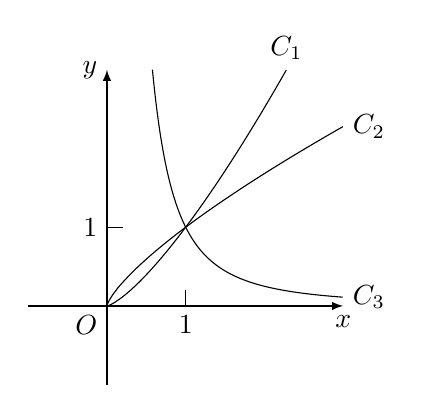
\begin{tikzpicture}[>=latex]
        \draw [->] (-1,0) -- (3,0) node [below] {$x$};
        \draw [->] (0,-1) -- (0,3) node [left] {$y$};
        \draw (0,0) node [below left] {$O$};
        \draw (1,0.2) -- (1,0) node [below] {$1$};
        \draw (0.2,1) -- (0,1) node [left] {$1$};
        \draw [domain = {sqrt(3)/3}:3, samples = 400] plot (\x,{\x^(-2)});
        \draw [domain = 0:3, samples = 400] plot (\x,{\x^(3/4)});
        \draw [domain = 0:{3^(3/4)}, samples = 400] plot (\x,{\x^(4/3)});
        \draw (3,{1/9}) node [right] {$C_3$} (3,{3^(3/4)}) node [right] {$C_2$} ({3^(3/4)},3) node [above] {$C_1$};
    \end{tikzpicture}
\end{center}
\fourch{$\dfrac 43,-2,\dfrac 34$}{$-2,\dfrac 34,\dfrac 43$}{$-2,\dfrac 43,\dfrac 34$}{$\dfrac 34,\dfrac 43,-2$}
\item {\tiny (005460)}若幂函数$y=x^n$的图像在$0<x<1$时位于直线$y=x$的下方, 则$n$的取值范围是\blank{50}.
\item {\tiny (005461)}若幂函数$y=x^n$的图像在$0<x<1$时位于直线$y=x$的上方, 则$n$的取值范围是\blank{50}.
\item {\tiny (005463)}幂函数$y=x^p$与$y=x^q$的图像都通过定点\blank{50}, 它们在第一象限部分关于直线$y=x$对称, 则$p,q$应满足的条件是\blank{50}.
\item {\tiny (005464)}若实数$a$满足$2.4^a>2.5^a$, 求$a$的取值范围.
\item {\tiny (005544)}若幂函数$f(x)$是奇函数, 则$f^{-1}(1)=$\blank{50}, $f^{-1}(-1)=$\blank{50}.
\item {\tiny (005560)}求函数$y=9^x-m\cdot 3^x+1$的最小值.
\item {\tiny (005561)}填写下表:
\begin{center}
    \begin{tabular}{|c|c|c|c|c|}
        \hline
        $x$	 & $f(x)=x^2$ & $f(x)-f(x-1)$ & $g(x)=2^x$ & $g(x)-g(x-1)$ \\ \hline
        $0$ & & & & \\ \hline
        $1$ & & & & \\ \hline
        $2$ & & & & \\ \hline
        $3$ & & & & \\ \hline
        $4$ & & & & \\ \hline
        $5$ & & & & \\ \hline
        $6$ & & & & \\ \hline
        $7$ & & & & \\ \hline
        $8$ & & & & \\ \hline
        $9$ & & & & \\ \hline
        $10$ & & & & \\ \hline
    \end{tabular}
\end{center}
(1) 比较$f(x)=x^2$与$g(x)=2^x$的函数值的大小;\\
(2) 比较$f(x)=x^2$与$g(x)=2^x$的函数值递增的快慢.
\item {\tiny (005562)}已知函数$f(x)=2x+1$, $g(x)=1.5^x$, $h(x)=x^{1.5}$, 试用数值计算比较三个函数在$[0,+\infty)$上的函数值的大小、图像递增的快慢. 并说明在函数图像上的表现.
解  列表并计算得:
\begin{center}
    \begin{longtable}{|c|c|c|c|c|c|c|}
        \hline
        $x$	 & $f(x)=2x+1$ & $f(x)-f(x-1)$ & $g(x)=1.5^x$ & $g(x)-g(x-1)$ & $h(x)=x^{1.5}$ & $h(x)-h(x-1)$ \\ \hline
        \endhead
        $0$ & $1$ & & $1$ & & $0$ &  \\ \hline
        $1$ & $3$ & $2$ & $1.5$ & $0.5$ & $1$ & $1$\\ \hline
        $2$ & $5$ & $2$ & $2.25$ & $0.75$ & $2.82842712$ & $1.82842712$\\ \hline
        $3$ & $7$ & $2$ & $3.375$ & $1.125$ & $5.19615242$ & $2.3677253$\\ \hline
        $4$ & $9$ & $2$ & $5.0625$ & $1.6875$ & $8$ & $2.80384758$\\ \hline
        $5$ & $11$ & $2$ & $7.59375$ & $2.53125$ & $11.1803399$ & $3.18033989$\\ \hline
        $6$ & $13$ & $2$ & $11.390625$ & $3.796875$ & $14.6969385$ & $3.51659857$\\ \hline
        $7$ & $15$ & $2$ & $17.085938$ & $5.6953125$ & $18.5202592$ & $3.82332072$\\ \hline
        $8$ & $17$ & $2$ & $25.628906$ & $8.5429688$ & $22.627417$ & $4.10715782$\\ \hline
        $9$ & $19$ & $2$ & $38.443359$ & $12.814453$ & $27$ & $4.372583$\\ \hline
        $10$ & $21$ & $2$ & $57.665039$ & $19.22168$ & $31.6227766$ & $4.6227766$\\ \hline
        $11$ & $23$ & $2$ & $86.497559$ & $28.83252$ & $36.4828727$ & $4.86009609$\\ \hline
        $12$ & $25$ & $2$ & $129.74634$ & $43.248779$ & $41.5692194$ & $5.08634669$\\ \hline
        $13$ & $27$ & $2$ & $194.61951$ & $64.873169$ & $46.8721666$ & $5.3029472$\\ \hline
        $14$ & $29$ & $2$ & $291.92926$ & $97.309753$ & $52.3832034$ & $5.51103683$\\ \hline
        $15$ & $31$ & $2$ & $437.89389$ & $145.96463$ & $58.0947502$ & $5.71154678$\\ \hline
        $16$ & $33$ & $2$ & $656.84084$ & $218.94695$ & $64$ & $5.90524981$\\ \hline
        $17$ & $35$ & $2$ & $985.26125$ & $328.42042$ & $70.0927956$ & $6.09279564$\\ \hline
        $18$ & $37$ & $2$ & $1477.8919$ & $492.63063$ & $76.3675324$ & $6.27473673$\\ \hline
        $19$ & $39$ & $2$ & $2216.8378$ & $738.94594$ & $82.8190799$ & $6.45154756$\\ \hline
        $20$ & $41$ & $2$ & $3325.2567$ & $1108.4189$ & $89.4427191$ & $6.62363917$\\ \hline
        $21$ & $43$ & $2$ & $4987.8851$ & $1662.6284$ & $96.2340896$ & $6.79137049$\\ \hline
        $22$ & $45$ & $2$ & $7481.8276$ & $2493.9425$ & $103.189147$ & $6.95505712$\\ \hline
        $23$ & $47$ & $2$ & $11222.741$ & $3740.9138$ & $110.304125$ & $7.11497832$\\ \hline
        $24$ & $49$ & $2$ & $16834.112$ & $5611.3707$ & $117.575508$ & $7.27138262$\\ \hline
        $25$ & $51$ & $2$ & $25251.168$ & $8417.0561$ & $125$ & $7.42449235$\\ \hline
        $26$ & $53$ & $2$ & $37876.752$ & $12625.584$ & $132.574507$ & $7.57450735$\\ \hline
        $27$ & $55$ & $2$ & $56815.129$ & $18938.376$ & $140.296115$ & $7.72160806$\\ \hline
        $28$ & $57$ & $2$ & $85222.693$ & $28407.564$ & $148.162073$ & $7.86595801$\\ \hline
        $29$ & $59$ & $2$ & $127834.04$ & $42611.346$ & $156.169779$ & $8.00770599$\\ \hline
        $30$ & $61$ & $2$ & $191751.06$ & $63917.02$ & $164.316767$ & $8.14698784$\\ \hline
        $\cdots$ & $\cdots$ & $\cdots$ & $\cdots$ & $\cdots$ & $\cdots$ & $\cdots$ \\ \hline
    \end{longtable}
\end{center}
得点$A,B,C,D$的横坐标分别约为$1.5,4.8, 6.5, 7.4$, 记作$x_A,x_B,x_C,x_D$.\\
(1) 三个函数的函数值的大小情况如下:\\
\textcircled{1} 当$0<x<x_A$时, $f(x)>g(x)>h(x)$;
\textcircled{2} 当$x_A<x<x_B$时, $f(x)>h(x)>g(x)$;
\textcircled{3} 由$x_B<x<x_C$时, $h(x)>f(x)>g(x)$;
\textcircled{4} 当$x_C<x<x_D$时, $h(x)>g(x)>f(x)$;
\textcircled{5} 当$x_D<x$时, $g(x)>h(x)>f(x)$;
\textcircled{6} 当$x=x_A$时, $f(x)>g(x)=h(x)$;
\textcircled{7} 当$x=x_B$时, $f(x)=h(x)>g(x)$;
\textcircled{8} 当$x=x_C$时, $f(x)=g(x)<h(x)$;
\textcircled{9} 当$x=x_D$时, $f(x)<g(x)=g(x)$.\\
(2) 它们在同一个平面直角坐标系下的图像如图14所示.
\begin{center}
    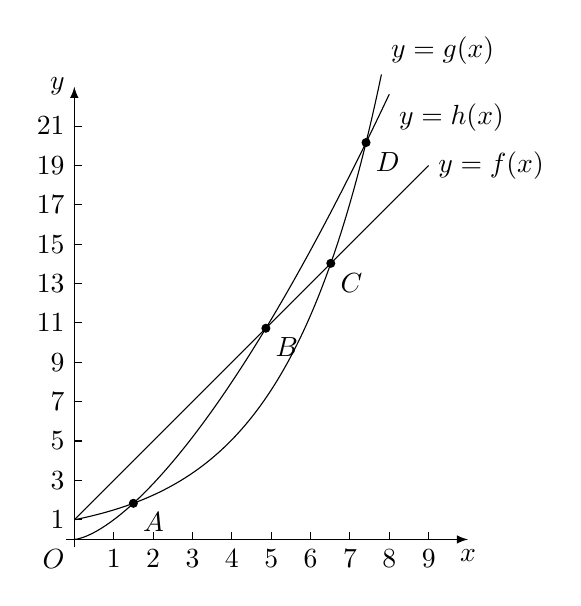
\begin{tikzpicture}[>=latex]
        \draw [->] (-0.1,0) -- (5,0) node [below] {$x$};
        \draw [->] (0,-0.1) -- (0,5.75) node [left] {$y$};
        \draw (0,0) node [below left] {$O$};
        \draw [domain = 0:9,samples = 100, name path = firstorder] plot ({\x/2},{(2*\x+1)/4});
        \draw (4.5,{19/4}) node [right] {$y=f(x)$};
        \draw [domain = 0:7.8, samples = 100, name path = exponential] plot ({\x/2},{1.5^(\x)/4}); 
        \draw (3.9,{1.5^7.8/4}) node [above right] {$y=g(x)$};
        \draw [domain = 0:8, samples = 100, name path = power] plot ({\x/2},{\x^(3/2)/4});
        \draw (4,{8^(3/2)/4}) node [below right] {$y=h(x)$};
        \path [name intersections = {of = firstorder and exponential, by = {T,C}}];
        \path [name intersections = {of = firstorder and power, by = B}];
        \path [name intersections = {of = exponential and power, by = {A,D}}];
        \filldraw (A) circle (0.05) node [below right] {$A$};
        \filldraw (B) circle (0.05) node [below right] {$B$};
        \filldraw (C) circle (0.05) node [below right] {$C$};
        \filldraw (D) circle (0.05) node [below right] {$D$};
        \foreach \i in {1,2,...,9}{\draw (\i/2,0.1) -- (\i/2,0) node [below] {$\i$};};
        \foreach \i in {1,3,...,21}{\draw (0.1,\i/4) -- (0,\i/4) node [left] {$\i$};};
    \end{tikzpicture}
\end{center}
由表格及图像可看出, 三个函数的函数值变化及相应增量规律为: 随着$x$的增大, 直线型均匀上升, 增量恒定; 指数型急剧上升, 在区间$[0,+\infty)$上递增增量快速增大; 幂函数型虽上升较快, 但随着$x$的不断增大上升趋势远不如指数型, 几乎微不足道, 其增量缓慢递增.
\item {\tiny (005564)}下列函数中, 值域为$(0,+\infty)$的函数是\bracket{20}.
\fourch{$y=(\dfrac 18)^{2-x}$}{$y=\sqrt {1-3^x}$}{$y=\sqrt {(\dfrac 13)^x-1}$}{$y=2^{\frac 1{3-x}}$}
\item {\tiny (005566)}下列函数式中, 满足$f(x+1)=2f(x)$的$f(x)$是\bracket{20}.
\fourch{$\dfrac 12(x+1)$}{$x+\dfrac 14$}{$2^x$}{$2^{-x}$}
\item {\tiny (005567)}若$f(x)=\dfrac{\mathrm{e}^x-\mathrm{e}^{-x}}2$, $g(x)=\dfrac{\mathrm{e}^x+\mathrm{e}^{-x}}2$.则下列关系式中不正确的是\bracket{20}.
\twoch{$[g(x)]^2-[f(x)]^2=1$}{$f(2x)=2f(x)\cdot g(x)$}{$g(2x)=[f(x)]^2+[g(x)]^2$}{$f(-x)g(x)=f(x)g(-x)$}
\item {\tiny (005568)}若$a>b$且$ab\ne 0$.则在\textcircled{1} $a^2>b^2$, \textcircled{2} $2^a>2^b$, \textcircled{3} $\dfrac 1a<\dfrac 1b$, \textcircled{4} $a^{\frac 13}>b^{\frac 13}$, \textcircled{5} $(\dfrac 13)^a<(\dfrac 13)^b$这五个关系式中, 恒成立的有\bracket{20}.
\fourch{$1$个}{$2$个}{$3$个}{$4$个}
\item {\tiny (005569)}在同一平面直角坐标系中, 函数$f(x)=ax$与$g(x)=a^x$的图像可能是\bracket{20}.
\fourch{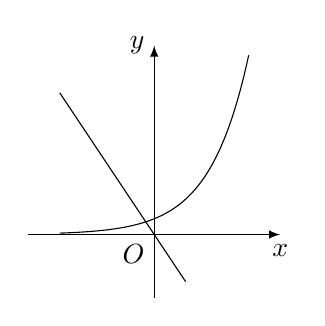
\begin{tikzpicture}[scale = 0.2, >=latex]
    \draw [->] (-8,0) -- (8,0) node [below] {$x$};
    \draw [->] (0,-4) -- (0,12) node [left] {$y$};
    \draw (0,0) node [below left] {$O$};
    \draw [domain = -6:2, samples = 100] plot (\x,{-1.5*\x});
    \draw [domain = -6:6, samples = 100] plot (\x,{1.5^\x});
\end{tikzpicture}}{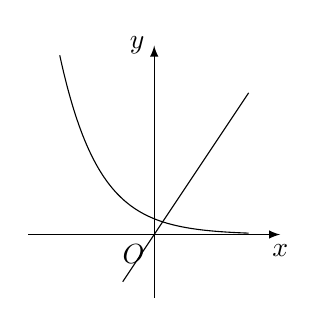
\begin{tikzpicture}[scale = 0.2, >=latex]
    \draw [->] (-8,0) -- (8,0) node [below] {$x$};
    \draw [->] (0,-4) -- (0,12) node [left] {$y$};
    \draw (0,0) node [below left] {$O$};
    \draw [domain = -2:6, samples = 100] plot (\x,{1.5*\x});
    \draw [domain = -6:6, samples = 100] plot (-\x,{1.5^\x});
\end{tikzpicture}}{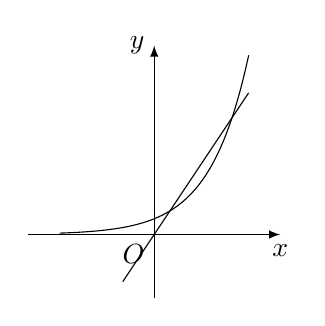
\begin{tikzpicture}[scale = 0.2, >=latex]
    \draw [->] (-8,0) -- (8,0) node [below] {$x$};
    \draw [->] (0,-4) -- (0,12) node [left] {$y$};
    \draw (0,0) node [below left] {$O$};
    \draw [domain = -2:6, samples = 100] plot (\x,{1.5*\x});
    \draw [domain = -6:6, samples = 100] plot (\x,{1.5^\x});
\end{tikzpicture}}{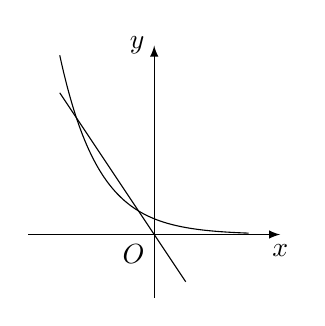
\begin{tikzpicture}[scale = 0.2, >=latex]
    \draw [->] (-8,0) -- (8,0) node [below] {$x$};
    \draw [->] (0,-4) -- (0,12) node [left] {$y$};
    \draw (0,0) node [below left] {$O$};
    \draw [domain = -2:6, samples = 100] plot (-\x,{1.5*\x});
    \draw [domain = -6:6, samples = 100] plot (-\x,{1.5^\x});
\end{tikzpicture}}
\item {\tiny (005571)}若$f(x)$在$(0,+\infty)$上是减函数, 而$f(a^x)$在$(-\infty ,+\infty)$上是增函数, 则实数$a$的取值范围是\bracket{20}.
\fourch{(0, 1)}{$(0,1)\cup (1,+\infty)$}{$(0,+\infty)$}{$(1,+\infty)$}
\item {\tiny (005573)}若函数$f(x)=(a^2-1)^x$在$(-\infty ,+\infty)$上是减函数, 则$a$的取值范围是\bracket{20}.
\fourch{$|a|>1$}{$|a|<\sqrt 2$}{$a>\sqrt 2$}{$1<|a|<\sqrt 2$}
\item {\tiny (005574)}若函数$f(x)=a^x-(b+1)$($a>0$且$a\ne 1$)的图像在第一、三、四象限, 则必有\bracket{20}.
\fourch{$0<a<1$且$b>0$}{$0<a<1$且$b<0$}{$a>1$且$b<1$}{$a>1$且$b>0$}
\item {\tiny (005577)}根据条件确定实数$x$的取值范围:\\
(1) $2^x>0.5$:\blank{50};\\
(2) $2^x<1$:\blank{50};\\
(3) $0.2^{2x-1}>\dfrac 1{25}$:\blank{50};\\
(4) $8<(\dfrac 12)^{2x+1}$:\blank{50};\\
(5) $(a^2+a+2)^x>(a^2+a+2)^{1-x}$:\blank{50};\\
(6) $(\dfrac 12)^{x^2+x-2}<1$:\blank{50}.
\item {\tiny (005579)}若函数$f(x)$的定义域是$(0, 1)$, 则函数$f(2^{-x})$的定义域是\blank{50}, $f(3\times 9^x+2\times 3^x)$的定义域是\blank{50}.
\item {\tiny (005586)}函数$f(x)=a^{2x}-3a^x+2$($a>0$且$a\ne 1$)的最小值为\blank{50}.
\item {\tiny (005588)}函数$f(x)=\dfrac 1{3^x-1}$的值域是\blank{50}.
\item {\tiny (005589)}函数$f(x)=\dfrac{3^x}{3^x+1}$的值域是\blank{50}.
\item {\tiny (005590)}若关于$x$的方程$5^x=\dfrac{a+3}{5-a}$有负根, 则实数$a$的取值范围是\blank{50}.
\item {\tiny (005591)}若$0<a<1$, $x>y>1$, 则$a^x$, $x^a$, $a^y$, $y^a$从小到大的排列顺序是\blank{50}.
\item {\tiny (005592)}若$0.9<a<1$, 则$a$, $a^a$, $a^{a^a}$从小到大的排列顺序是\blank{50}.
\item {\tiny (005594)}若$f(x)=a+\dfrac 1{4^x+1}$是奇函数, 求常数$a$的值.
\item {\tiny (005595)}若$f(x)=x^2(\dfrac 1{a^x-1}+m)$($a>0$且$a\ne 1$)为奇函数, 求常数$m$的值.
\item {\tiny (005596)}已知函数$f(x)=(\dfrac 1{2^x-1}+\dfrac 12)x^3$.\\
(1) 求函数的定义域;\\
(2) 讨论$f(x)$的奇偶性;\\
(3) 求证: $f(x)>0$.
\item {\tiny (005597)}已知$f(x)=\dfrac{a^x-1}{a^x+1}$($a>1$).\\
(1) 判断函数$f(x)$的奇偶性;\\
(2) 求函数$f(x)$的值域;\\
(3) 求证: $f(x)$在区间$(-\infty ,+\infty)$上是增函数.
\item {\tiny (005598)}若$0\le x\le 2$, 求函数$y=4^{x-\frac 12}-3\cdot 2^x+5$的最大值和最小值.
\item {\tiny (005599)}若函数$f(x)=a^{2x}+2a^x-1$($a>0$且$a\ne 1$)在$[-1, 1]$上的最大值为$14$, 求实数$a$的值.
\item {\tiny (005600)}已知函数$f(x)=\dfrac a{a^2-2}(a^x-a^{-x})$($a>0$且$a\ne 1$)在$(-\infty ,+\infty)$上是增函数, 求实数$a$的取值范围.
\item {\tiny (005602)}已知集合$M=\{x|(x+1)^2\le 1\}$, $P=\{y|y=4^x-a\cdot 2^{x+1}+1,\ x\in M,\ \dfrac 34<a\le 1\}$, 且全集$U=\mathbf{R}$, 求$\complement _U(M\cup P)$.
\item {\tiny (005603)}求方程$x^{\frac 13}+2^x=0$的实根个数.
\item {\tiny (005604)}求关于$x$的方程$a^x+1=-x^2+2x+2a$($a>0$且$a\ne 1$)的实数解的个数.
\item {\tiny (005605)}在同一个平面直角坐标系中, 作出$t(x)=0.5x$与$g(x)=0.2\times 2^x$的图像, 并比较它们的增长情况.
\item {\tiny (005606)}某地区不同身高的未成年男性的体重平均值如下表(身高: $\text{cm}$; 体重: $\text{kg}$):
\begin{center}
    \begin{tabular}{|c|c|c|c|c|c|c|}
        \hline
        身高 & $60$ & $70$ & $80$ & $90$ & $100$ & $110$\\ \hline
        体重 & $6.13$ & $7.90$ & $9.99$ & $12.15$ & $15.02$ & $17.05$\\ \hline
        身高 & $120$ & $130$ & $140$ & $150$ & $160$ & $170$\\ \hline
        体重 & $20.92$ & $26.86$ & $31.11$ & $38.85$ & $47.25$ & $55.05$\\ \hline
    \end{tabular}
\end{center}
为了揭示未成年男性的身高与体重的规律, 甲选择了模型$y=ax^2+bx+c$($a>0$), 乙选择了模型$y=ba^x$($a>1$), 其中$y$表示体重, $x$表示身高.你认为谁选择的模型较好?
\item {\tiny (005607)}用计算器计算并填写下表:
\begin{center}
    \begin{tabular}{|c|c|c|c|c|}
        \hline
        $x$	& $f(x)=x^{\frac 12}$ & $g(x)=x^{0.6}$ & $h(x)=2.1^x$ & $s(x)=2.2^x$ \\ \hline
        $0$ & & & & \\ \hline
        $1$ & & & & \\ \hline
        $2$ & & & & \\ \hline
        $3$ & & & & \\ \hline
        $4$ & & & & \\ \hline
        $5$ & & & & \\ \hline
        $6$ & & & & \\ \hline
        $7$ & & & & \\ \hline
        $8$ & & & & \\ \hline
        $9$ & & & & \\ \hline
        $10$ & & & & \\ \hline
    \end{tabular}
\end{center}
从表中变化的现象可以归纳出哪些函数递增的规律?\\
(1) 幂函数$f(x)$与$g(x)$之间比较得出的规律;
(2) 指数函数$h(x)$与$s(x)$之间比较得出的规律;
(3) 幂函数$f(x)=x^{\frac 12}$与指数函数$h(x)$之间比较得出的规律
\item {\tiny (005608)}求$\log_927$的值.
\item {\tiny (005609)}设$3^a=4^b=36$, 求$\dfrac 2a+\dfrac 1b$的值.
\item {\tiny (005610)}已知$x=a^{\frac 1{1-\log_ay}}$, $y=a^{\frac 1{1-\log_az}}$求证: $z=a^{\frac 1{1-\log_ax}}$.
\item {\tiny (005611)}已知$\log_{12}27=a$, 求$\log_616$.
\item {\tiny (005612)}若$a=b^2$($b>0$, $b\ne 1$), 则有\bracket{20}.
\fourch{$\log_2a=b$}{$\log_2b=a$}{$\log_ab=2$}{$\log_ba=2$}
\item {\tiny (005613)}若$\log_x\sqrt[7]y=z$, 则$x,y,z$之间满足\bracket{20}.
\fourch{$y^7=x^z$}{$y=x^{7z}$}{$y=7x^z$}{$y=z^{7x}$}
\item {\tiny (005614)}$2^{\log_43}$的值等于\bracket{20}.
\fourch{3}{$\sqrt 3$}{$\dfrac{\sqrt 3}3$}{$\dfrac 13$}
\item {\tiny (005615)}$\log_ab\cdot \log_3a=5$, 则$b=$\bracket{20}.
\fourch{$a^3$}{$a^5$}{$3^5$}{$5^3$}
\item {\tiny (005616)}若点$P(\lg a,\lg b)$关于$x$轴的对称点的坐标是(0, -1), 则$a$和$b$的值是\bracket{20}.
\fourch{$a=1$, $b=10$}{$a=1$, $b=\dfrac 1{10}$}{$a=10$, $b=1$}{$a=\dfrac 1{10}$, $b=1$}
\item {\tiny (005617)}给出下列四个式子(已知$a>0$, $a\ne 1$, $x>y>0$): \textcircled{1} $\log_ax\cdot \log_ay=\log_a(x+y)$; \textcircled{2} $\log_ax+\log_ay=\log_a(x+y)$; \textcircled{3} $\log_a\dfrac xy=\log_a(x-y)$; \textcircled{4} $\log_a(x-y)=\dfrac{\log_ax}{\log_ay}$.其中正确的有\bracket{20}.
\fourch{$0$个}{$1$个}{$2$个}{$3$个}
\item {\tiny (005618)}若$m>0$, 且$10^x=\lg (10m)+\lg \dfrac 1m$, 则$x$的值为\bracket{20}.
\fourch{$2$}{$1$}{$0$}{$-1$}
\item {\tiny (005619)}若$\lg x=a$, $\lg y=b$, 则$\lg \sqrt x-\lg (\dfrac y{10})^2$的值等于\bracket{20}.
\fourch{$\dfrac 12a-2b-2$}{$\dfrac 12a-2b+2$}{$\dfrac 12a-2b-1$}{$\dfrac 12a-2b+1$}
\item {\tiny (005620)}如果方程$\lg ^2x+(\lg 2+\lg 3)\lg x+\lg 2\cdot \lg 3=0$的两个根为$x_1,x_2$, 那么$x_1\cdot x_2$的值为\bracket{20}.
\fourch{$\lg 2\cdot \lg 3$}{$\lg 2+\lg 3$}{$\dfrac 16$}{$-6$}
\item {\tiny (005621)}若$x=t^{\frac 1{t-1}}$, $y=t^{\frac t{t-1}}$($t>0$, $t\ne 1$), 则$x,y$之间的关系是\bracket{20}.
\fourch{$y^x=x^{\frac 1y}$}{$y^{\frac 1x}=x^y$}{$y^x=x^y$}{$x^x=y^y$}
\item {\tiny (005622)}若$\log_8x=-\dfrac 23$, 则$x=$\blank{50}.
\item {\tiny (005623)}若$\log_x27=\dfrac 34$, 则$x=$\blank{50}.
\item {\tiny (005624)}若$\log_2(\log_5x)=0$, 则$x=$\blank{50}.
\item {\tiny (005625)}若$\log_2(\lg x)=1$, 则$x=$\blank{50}.
\item {\tiny (005626)}若$\log_2[\log_3(\log_5x)]=0$, 则$x=$\blank{50}.
\item {\tiny (005627)}若$\log_2[\log_3(\log_4x)]=\log_3[\log_4(\log_2y)]=\log_4[\log_2(\log_3z)]=0$.则$x+y+z=$\blank{50}.
\item {\tiny (005628)}计算: $2^{\log_4(2-\sqrt 3)^2}+3^{\log_9(2+\sqrt 3)^2}=$\blank{50}.
\item {\tiny (005629)}计算: $2^{1+\dfrac 12\log_25}=$\blank{50}.
\item {\tiny (005630)}计算: $9^{\log_32}=$\blank{50}.
\item {\tiny (005631)}计算: $5^{3-2\log_{25}125}=$\blank{50}.
\item {\tiny (005632)}计算: $\log_{(2-\sqrt 3)}(7+4\sqrt 3)=$\blank{50}.
\item {\tiny (005633)}计算: $\log_6(\sqrt {2+\sqrt 3}+\sqrt {2-\sqrt 3})=$\blank{50}.
\item {\tiny (005634)}计算: $(2+\sqrt 3)^{-1}-\log_{(2+\sqrt 3)}(7+4\sqrt 3)=$\blank{50}.
\item {\tiny (005635)}计算: $-2^2\div (-\dfrac{27}8)^{-\frac 13}-(0.7)^{\lg 1}+\log_3\dfrac 14+\log_312=$\blank{50}.
\item {\tiny (005636)}若$3^x=12^y=8$, 则$\dfrac 1x-\dfrac 1y=$\blank{50}.
\item {\tiny (005637)}若$2^x=7^y=196$, 则$\dfrac 1x+\dfrac 1y=$\blank{50}.
\item {\tiny (005639)}已知正数$a,b$满足$a^2+b^2=7ab$, 求证: $\log_m\dfrac{a+b}3=\dfrac 12(\log_ma+\log_mb)$($m>0$, $m\ne 1$).
\item {\tiny (005640)}已知$\log_a(x^2+1)+\log_a(y^2+4)=\log_a8+\log_ax+\log_ay$($a>0$, $a\ne 1$), 求$\log_8(xy)$的值.
\item {\tiny (005641)}已知只有一个$x$的值满足方程$(1-\lg ^2a)x^2+(1-\lg a)x+2=0$, 求实数$a$的值.
\item {\tiny (005642)}设方程$x^2-\sqrt {10}x+2=0$的两个根为$\alpha ,\beta$, 求$\log_4\dfrac{\alpha ^2-\alpha \beta +\beta ^2}{(\alpha -\beta)^2}$的值.
\item {\tiny (005643)}已知$\lg a$和$\lg b$是关于$x$的方程$x^2-x+m=0$的两个根, 且关于$x$的方程$x^2-(\lg a)x-(1+\lg a)=0$有两个相等的实数根, 求实数$a,b$和$m$的值.
\item {\tiny (005644)}已知函数$f(x)=x^2\lg a+2x+4\lg a$的最大值为3, 求实数$a$的值.
\item {\tiny (005645)}已知函数$f(x)=x^2+(\lg a+2)x+\lg b$, 满足$f(-1)=-2$, 且对一切实数$x$都有$f(x)\ge 2x$, 求实数$a,b$的值.
\item {\tiny (005646)}已知$2\lg \dfrac{x-y}2=\lg x+\lg y$, 求$\dfrac xy$的值.
\item {\tiny (005647)}设$A>B>0$, $A^2+B^2=6AB$, 求证: $\log_a\dfrac{A-B}2=\dfrac 12(\log_aA+\log_aB)$($a>0$且$a\ne 1$).
\item {\tiny (005648)}已知集合$M=\{x,xy,\lg (xy)\}$, $P=\{0,|x|,y\}$, 且满足$M=P$, 求实数$x,y$的值.
\item {\tiny (005649)}已知$12^x=3$, $12^y=2$, 求$8^{\frac{1-2x}{1-x+y}}$的值.
\item {\tiny (005650)}已知不相等的两个正数$a,b$满足$a^{\lg ax}=b^{\lg bx}$, 求$(ab)^{\lg abx}$的值.
\item {\tiny (005651)}已知$x,y,z>0$, 且$\lg x+\lg y+\lg z=0$, 求$x^{\frac 1{\lg y}+\dfrac 1{\lg z}}\cdot y^{\frac 1{\lg z}+\dfrac 1{\lg x}}\cdot z^{\frac 1{\lg x}+\dfrac 1{\lg y}}$的值.
\item {\tiny (005652)}求$y^{\lg 20}\cdot (\dfrac 12)^{\lg 0.7}$的值.
\item {\tiny (005653)}化简$\dfrac{\log_58}{\log_52}$可得\bracket{20}.
\fourch{$\log_54$}{$3\log_52$}{$\log_36$}{$3$}
\item {\tiny (005654)}$\dfrac{\log_89}{\log_23}$的值是\bracket{20}.
\fourch{$\dfrac 23$}{$1$}{$\dfrac 32$}{$2$}
\item {\tiny (005655)}若$\log_ab=\log_ba$($a\ne b$, $a\ne 1$, $b\ne 1$), 则$ab$等于\bracket{20}.
\fourch{$1$}{$2$}{$\dfrac 14$}{$4$}
\item {\tiny (005656)}$\dfrac 1{\log_{\frac 12}\dfrac 13}+\dfrac 1{\log_{\frac 15}\dfrac 13}$的值所属区间是\bracket{20}.
\fourch{$(-2, -1)$}{$(1, 2)$}{$(-\infty ,-2)$}{$(2, 3)$}
\item {\tiny (005657)}若$\log_37\cdot \log_29\cdot \log_{49}m=\log_4\dfrac 12$, 则$m$的值等于\bracket{20}.
\fourch{$\dfrac 14$}{$\dfrac{\sqrt 2}2$}{$\sqrt 2$}{$4$}
\item {\tiny (005658)}若$x\ne 1$, 则与$\dfrac 1{\log_3x}+\dfrac 1{\log_4x}+\dfrac 1{\log_5x}$相等的式子是\bracket{20}.
\fourch{$\dfrac 1{\log_{60}x}$}{$\dfrac 1{\log_3x\cdot \log_4x\cdot \log_5x}$}{$\dfrac 1{\log_x60}$}{$\dfrac{12}{\log_3 x+\log_4 x+\log_5 x}$}
\item {\tiny (005659)}若$\log_83=p$, $\log_35=q$, 则$\lg 5$(用$p,q$表示)等于\bracket{20}.
\fourch{$\dfrac{3p+q}5$}{$\dfrac{1+3pq}{p+q}$}{$\dfrac{3pq}{1+3pq}$}{$p^2+q^2$}
\item {\tiny (005660)}已知$x,y,z$都是大于$1$的正数, $m>0$, 且$\log_xm=24$, $\log_ym=40$, $\log_{xyz}m=12$, 则$\log_zm$的值为\bracket{20}.
\fourch{$\dfrac 1{60}$}{$60$}{$\dfrac{200}3$}{$\dfrac 3{20}$}
\item {\tiny (005661)}计算: $\log_{64}32=$\blank{50}.
\item {\tiny (005662)}计算: $\log_{\frac 1a}b+\log_ab=$\blank{50}.
\item {\tiny (005663)}计算: $\log_625\cdot \log_53\cdot \log_96=$\blank{50}.
\item {\tiny (005664)}计算: $(\log_25+\log_40.2)(\log_52+\log_{25}0.5)=$\blank{50}.
\item {\tiny (005665)}计算: $\log_2\dfrac 1{25}\cdot \log_3\dfrac 18\cdot \log_5\dfrac 19=$\blank{50}.
\item {\tiny (005666)}计算: $a^{\frac{\log_b(\log_ba)}{\log_ba}}=$\blank{50}.
\item {\tiny (005667)}计算: $a^{\frac{\log_ma-\log_mb}{\log_ma}}=$\blank{50}.
\item {\tiny (005668)}已知$n\in \mathbf{N}^*$, 计算: $(\log_23+\log_49+\log_827+\cdots +\log_{2^n}3^n)\cdot \log_9\sqrt [n]{32}=$\blank{50}.
\item {\tiny (005669)}已知$\log_ax=2$, $\log_bx=1$, $\log_cx=4$, 则$\log_{abc}x=$\blank{50}.
\item {\tiny (005670)}已知$m=\log_25$, 则$2^m-m\lg 2-4=$\blank{50}.
\item {\tiny (005671)}已知$\lg (3x^3)-\lg (3y^3)=9$, 则$\dfrac xy=$\blank{50}.
\item {\tiny (005672)}记$\log_827=m$, 用$m$表示$\log_616$.
\item {\tiny (005673)}已知$\log_37=a$, $\log_34=b$, 求$\log_{12}21$.
\item {\tiny (005674)}已知$\log_23=a$, $\log_35=b$, 求$\log_{15}20$.
\item {\tiny (005675)}已知$a>b>1$, $\log_ab+\log_ba=\dfrac{10}3$, 求$\log_ab-\log_ba$的值.
\item {\tiny (005676)}已知$\log_{2a}a=m$, $\log_{3a}2a=n$, 求证: $2^{1-mn}=3^{n-mn}$.
\item {\tiny (005677)}已知关于$x$的方程$x^2-(\log_2b+\log_a2)x+\log_ab=0$的两根为$-1$和$2$, 求实数$a,b$的值.
\item {\tiny (005678)}已知$a^2+b^2=c^2$, 求证$\log_{(c+b)}a+\log_{(c-b)}a=2\log_{(c+b)}a\cdot \log_{(c-b)}a$.
\item {\tiny (005679)}已知正实数$x,y,z$满足$3^x=4^y=6^z$.\\
(1) 求证$\dfrac 1z-\dfrac 1x=\dfrac 1{2y}$;\\
(2) 比较$3x,4y,6z$的大小.
\item {\tiny (005680)}求函数$y=\dfrac{\sqrt {\log_{0.8}x-1}}{2x-1}$的定义域.
\item {\tiny (005681)}解不等式$\log_{0.2}(x^2+2x-3)>\log_{0.2}(3x+1)$.
\item {\tiny (005682)}将$\log_{0.7}0.8$, $\log_{1.1}0.9$, $1.1^{0.9}$由小到大排列.
\item {\tiny (005683)}若$0<x<1$, $a>0$, $a\ne 1$, 比较$p=|\log_a(1-x)|$和$q=|\log_a(1+x)|$的大小.
\item {\tiny (005684)}求函数$f(x)=\log_{0.2}(x-1)(x+2)$为增函数的区间.
\item {\tiny (005685)}求函数$f(x)=\log_{\frac 12}(x^2-6x+17)$的值域.
\item {\tiny (005686)}已知关于$x$的方程$ax^2-4ax+1=0$的两个实数根$\alpha ,\beta$满足不等式$|\lg \alpha -\lg \beta|\le 1$, 求实数$a$的取值范围.
\item {\tiny (005687)}与函数$y=x$为同一个函数的是\bracket{20}.
\twoch{$y=\sqrt {x^2}$}{$y=\dfrac{x^2}x$}{$y=a^{\log_ax}$($a>0$且$a\ne 1$)}{$y=\log_aa^x$($a>0$且$a\ne 1$)}
\item {\tiny (005688)}若函数$y=f(x)$的反函数是$y=\lg (x-1)+3$($x>1$), 则$f(x)$等于\bracket{20}.
\fourch{$10^{x+3}+1$}{$10^{x-3}-1$}{$10^{x+3}-1$}{$10^{x-3}+1$}
\item {\tiny (005689)}若函数$f(x)=\log_2x+3$($x\ge 1$), 则其反函数$f^{-1}(x)$的定义域是\bracket{20}.
\fourch{$\mathbf{R}$}{$\{x|x\ge 1\}$}{$\{x|0<x<1\}$}{$\{x|x\ge 3\}$}
\item {\tiny (005690)}图中图像所对应的函数可能是\bracket{20}.
\begin{center}
    \begin{tikzpicture}[>=latex]
        \draw [->] (-1,0) -- (3,0) node [below] {$x$};
        \draw [->] (0,-2) -- (0,2) node [left] {$y$};
        \draw (0,0) node [below left] {$O$};
        \draw [domain = -1.4:1.8] plot ({0.5^\x},\x);
        \draw (1,0) node [below] {$1$}; 
    \end{tikzpicture}
\end{center}
\fourch{$y=2^x$}{$y=2^x$的反函数}{$y=2^{-x}$}{$y=2^{-x}$的反函数}
\item {\tiny (005691)}设$f(x)$是定义在$(-\infty ,+\infty)$上的偶函数, 且它在$[0,+\infty)$上是增函数, 记$a=f(-\log_{\sqrt 2}\sqrt 3)$, $b=f(-\log_{\sqrt 3}\sqrt 2)$, $c=f(-2)$, 则$a,b,c$的大小关系是\bracket{20}.
\fourch{$a>b>c$}{$b>c>a$}{$c>a>b$}{$c>b>a$}
\item {\tiny (005692)}下列函数图像中, 不正确的是\bracket{20}.
\begin{center}
    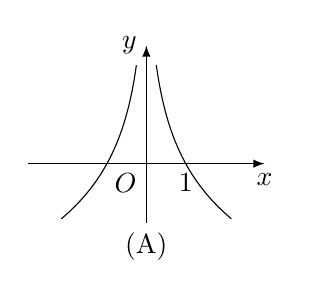
\begin{tikzpicture}[>=latex, scale = 0.5]
        \draw [->] (-3,0) -- (3,0) node [below] {$x$};
        \draw [->] (0,-1.5) -- (0,3) node [left] {$y$};
        \draw (0,0) node [below left] {$O$};
        \draw (1,0) node [below] {$1$};
        \draw [domain = -1.4:2.5] plot ({sqrt((1/3)^\x)},\x);
        \draw [domain = -1.4:2.5] plot ({-sqrt((1/3)^\x)},\x);
        \draw (0,-1.5) node [below] {(A)};
    \end{tikzpicture}
    \begin{tikzpicture}[>=latex, scale = 0.5]
        \draw [->] (-3,0) -- (3,0) node [below] {$x$};
        \draw [->] (0,-1.5) -- (0,3) node [left] {$y$};
        \draw (0,0) node [below left] {$O$};
        \draw (1,0) node [below] {$1$};
        \draw [domain = -0.9:2.5] plot ({-(1/3)^\x},\x);
        \draw (0,-1.5) node [below] {(B)};
    \end{tikzpicture}
    \begin{tikzpicture}[>=latex, scale = 0.5]
        \draw [->] (-3,0) -- (3,0) node [below] {$x$};
        \draw [->] (0,-1.5) -- (0,3) node [left] {$y$};
        \draw (0,0) node [below left] {$O$};
        \draw (1,0) node [below] {$1$};
        \draw [domain = -0.9:2.5] plot ({(1/3)^\x},{abs(\x)});
        \draw (0,-1.5) node [below] {(C)};
    \end{tikzpicture}
    \begin{tikzpicture}[>=latex, scale = 0.5]
        \draw [->] (-3,0) -- (3,0) node [below] {$x$};
        \draw [->] (0,-1.5) -- (0,3) node [left] {$y$};
        \draw (0,0) node [below left] {$O$};
        \draw (1,0) node [below] {$1$};
        \draw [domain = 0.1:2.5] plot (\x,{\x^(-1/3)});
        \draw (0,-1.5) node [below] {(D)};
    \end{tikzpicture}
\end{center}
\fourch{$y=\log_{\frac 13}x^2$}{$y=\log_{\frac 13}(-x)$}{$y=|\log_3x|$}{$y=|x^{-\frac 13}|$}
\item {\tiny (005693)}在同一平面直角坐标系中画出函数$y=x+a$与$y=\log_ax$的图像, 可能是\bracket{20}.
\fourch{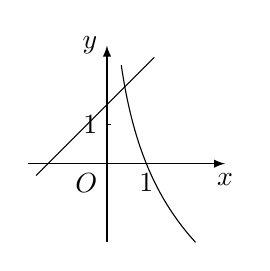
\begin{tikzpicture}[scale = 0.5, >=latex]
    \draw [->] (-2,0) -- (3,0) node [below] {$x$};
    \draw [->] (0,-2) -- (0,3) node [left] {$y$};
    \draw (0,0) node [below left] {$O$};
    \draw (1,0) node [below] {$1$};
    \draw (0.1,1) -- (0,1) node [left] {$1$};
    \draw [domain = -1.8:1.2] plot (\x,{\x+1.5});
    \draw [domain = -2.5:2] plot ({1.5^\x},{-\x}); 
\end{tikzpicture}}
{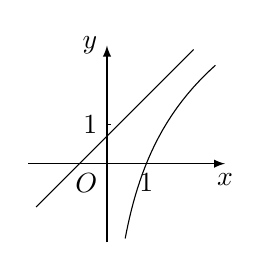
\begin{tikzpicture}[scale = 0.5, >=latex]
    \draw [->] (-2,0) -- (3,0) node [below] {$x$};
    \draw [->] (0,-2) -- (0,3) node [left] {$y$};
    \draw (0,0) node [below left] {$O$};
    \draw (1,0) node [below] {$1$};
    \draw (0.1,1) -- (0,1) node [left] {$1$};
    \draw [domain = -1.8:2.2] plot (\x,{\x+0.7}); 
    \draw [domain = -1.9:2.5] plot ({1.5^\x},{\x}); 
\end{tikzpicture}}
{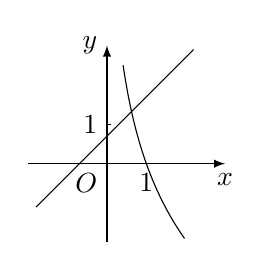
\begin{tikzpicture}[scale = 0.5, >=latex]
    \draw [->] (-2,0) -- (3,0) node [below] {$x$};
    \draw [->] (0,-2) -- (0,3) node [left] {$y$};
    \draw (0,0) node [below left] {$O$};
    \draw (1,0) node [below] {$1$};
    \draw (0.1,1) -- (0,1) node [left] {$1$};
    \draw [domain = -1.8:2.2] plot (\x,{\x+0.7}); 
    \draw [domain = -1.9:2.5] plot ({0.7^\x},{\x}); 
\end{tikzpicture}}
{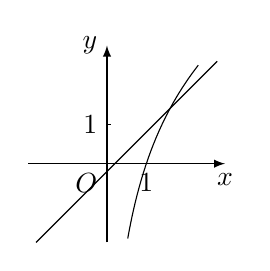
\begin{tikzpicture}[scale = 0.5, >=latex]
    \draw [->] (-2,0) -- (3,0) node [below] {$x$};
    \draw [->] (0,-2) -- (0,3) node [left] {$y$};
    \draw (0,0) node [below left] {$O$};
    \draw (1,0) node [below] {$1$};
    \draw (0.1,1) -- (0,1) node [left] {$1$};
    \draw [domain = -1.8:2.8] plot (\x,{\x-0.2}); 
    \draw [domain = -1.9:2.5] plot ({1.4^\x},{\x}); 
\end{tikzpicture}}
\item {\tiny (005694)}函数$y=f(x)$的图像如图所示, 则$y=\log_{0.7}f(x)$的示意图是\bracket{20}.
\begin{center}
    \begin{tikzpicture}[>=latex]
        \draw [->] (-0.5,0) -- (3,0) node [below] {$x$};
        \draw [->] (0,-0.5) -- (0,3) node [left] {$y$};
        \draw (0,0) node [below left] {$O$};
        \draw (1,0.1) -- (1,0) node [below] {$1$} (2,0.1) -- (2,0) node [below] {$2$} (0.1,1) -- (0,1) node [left] {$1$};
        \draw [dashed] (2,0) -- (2,3);
        \draw [dashed] (1,0) -- (1,1) -- (0,1);
        \draw [domain = 0.3:1.7] plot (\x,{3*(\x-1)^2+1});
    \end{tikzpicture}
\end{center}
\fourch{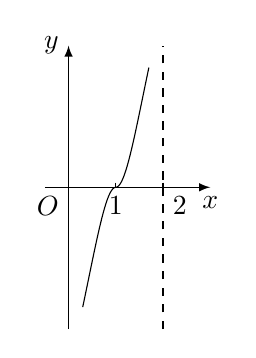
\begin{tikzpicture}[>=latex,scale = 0.6]
    \draw [->] (-0.5,0) -- (3,0) node [below] {$x$};
    \draw [->] (0,-3) -- (0,3) node [left] {$y$};
    \draw (0,0) node [below left] {$O$};
    \draw (1,0.1) -- (1,0) node [below] {$1$} (2,0.1) -- (2,0) node [below right] {$2$};
    \draw [dashed] (2,-3) -- (2,3);
    \draw [domain = 0.3:1] plot (\x,{ln(3*(\x-1)^2+1)/ln(0.7)});
    \draw [domain = 1:1.7] plot (\x,{-ln(3*(\x-1)^2+1)/ln(0.7)});
\end{tikzpicture}}{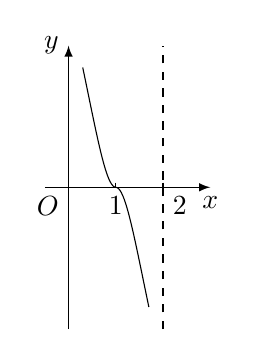
\begin{tikzpicture}[>=latex,scale = 0.6]
    \draw [->] (-0.5,0) -- (3,0) node [below] {$x$};
    \draw [->] (0,-3) -- (0,3) node [left] {$y$};
    \draw (0,0) node [below left] {$O$};
    \draw (1,0.1) -- (1,0) node [below] {$1$} (2,0.1) -- (2,0) node [below right] {$2$};
    \draw [dashed] (2,-3) -- (2,3);
    \draw [domain = 0.3:1] plot (\x,{-ln(3*(\x-1)^2+1)/ln(0.7)});
    \draw [domain = 1:1.7] plot (\x,{ln(3*(\x-1)^2+1)/ln(0.7)});
\end{tikzpicture}}{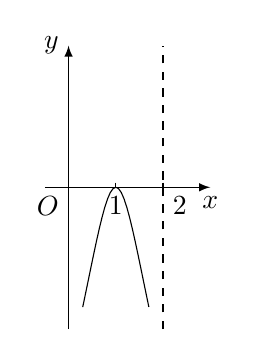
\begin{tikzpicture}[>=latex,scale = 0.6]
    \draw [->] (-0.5,0) -- (3,0) node [below] {$x$};
    \draw [->] (0,-3) -- (0,3) node [left] {$y$};
    \draw (0,0) node [below left] {$O$};
    \draw (1,0.1) -- (1,0) node [below] {$1$} (2,0.1) -- (2,0) node [below right] {$2$};
    \draw [dashed] (2,-3) -- (2,3);
    \draw [domain = 0.3:1.7] plot (\x,{ln(3*(\x-1)^2+1)/ln(0.7)});
\end{tikzpicture}}{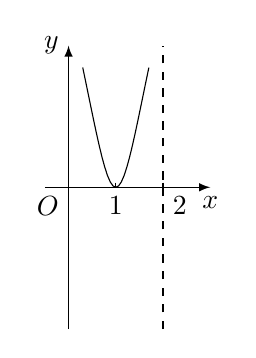
\begin{tikzpicture}[>=latex,scale = 0.6]
    \draw [->] (-0.5,0) -- (3,0) node [below] {$x$};
    \draw [->] (0,-3) -- (0,3) node [left] {$y$};
    \draw (0,0) node [below left] {$O$};
    \draw (1,0.1) -- (1,0) node [below] {$1$} (2,0.1) -- (2,0) node [below right] {$2$};
    \draw [dashed] (2,-3) -- (2,3);
    \draw [domain = 0.3:1.7] plot (\x,{-ln(3*(\x-1)^2+1)/ln(0.7)});
\end{tikzpicture}}
\item {\tiny (005695)}由关系式$\log_xy=3$所确定的函数$y=f(x)$的图像是\bracket{20}.
\fourch{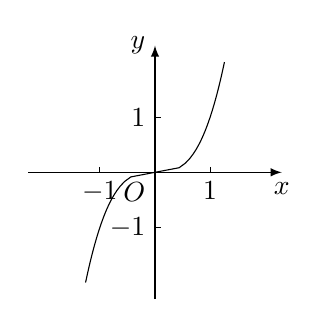
\begin{tikzpicture}[>=latex,scale = 0.7]
    \draw [->] (-2.3,0) -- (2.3,0) node [below] {$x$};
    \draw [->] (0,-2.3) -- (0,2.3) node [left] {$y$};
    \draw (0,0) node [below left] {$O$};
    \draw (1,0.1) -- (1,0) node [below] {$1$} (-1,0.1) -- (-1,0) node [below] {$-1$} (0.1,1) -- (0,1) node [left] {$1$} (0.1,-1) -- (0,-1) node [left] {$-1$};
    \draw [domain = 0:2] plot ({\x^(1/3)},\x);
    \draw [domain = 0:2] plot ({-\x^(1/3)},{-\x});
\end{tikzpicture}}{\begin{tikzpicture}[>=latex,scale = 0.7]
    \draw [->] (-2.3,0) -- (2.3,0) node [below] {$x$};
    \draw [->] (0,-2.3) -- (0,2.3) node [left] {$y$};
    \draw (0,0) node [below left] {$O$};
    \draw (1,0.1) -- (1,0) node [below] {$1$} (-1,0.1) -- (-1,0) node [below] {$-1$} (0.1,1) -- (0,1) node [left] {$1$} (0.1,-1) -- (0,-1) node [left] {$-1$};
    \draw [domain = 0:2] plot ({\x^(1/3)},\x);
    \filldraw [white] (0,0) circle (0.05) (1,1) circle (0.05);
    \draw (0,0) circle (0.05) (1,1) circle (0.05);
\end{tikzpicture}}{\begin{tikzpicture}[>=latex,scale = 0.7]
    \draw [->] (-2.3,0) -- (2.3,0) node [below] {$x$};
    \draw [->] (0,-2.3) -- (0,2.3) node [left] {$y$};
    \draw (0,0) node [below left] {$O$};
    \draw (1,0.1) -- (1,0) node [below] {$1$} (-1,0.1) -- (-1,0) node [below] {$-1$} (0.1,1) -- (0,1) node [left] {$1$} (0.1,-1) -- (0,-1) node [left] {$-1$};
    \draw [domain = 0:2] plot ({\x^(1/3)},\x);
\end{tikzpicture}}{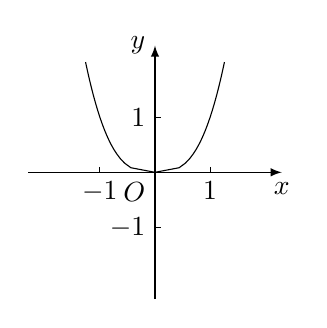
\begin{tikzpicture}[>=latex,scale = 0.7]
    \draw [->] (-2.3,0) -- (2.3,0) node [below] {$x$};
    \draw [->] (0,-2.3) -- (0,2.3) node [left] {$y$};
    \draw (0,0) node [below left] {$O$};
    \draw (1,0.1) -- (1,0) node [below] {$1$} (-1,0.1) -- (-1,0) node [below] {$-1$} (0.1,1) -- (0,1) node [left] {$1$} (0.1,-1) -- (0,-1) node [left] {$-1$};
    \draw [domain = 0:2] plot ({\x^(1/3)},\x);
    \draw [domain = 0:2] plot ({-\x^(1/3)},\x);
\end{tikzpicture}}
\item {\tiny (005696)}若函数$f(x)=\dfrac{1-2^x}{1+2^x}$, 则$f^{-1}(\dfrac 35)$等于\bracket{20}.
\fourch{$3$}{$2$}{$1$}{$-2$}
\item {\tiny (005697)}函数$y=\log_{\frac 13}(x^2-3x+4)$的定义域为\blank{50}.
\item {\tiny (005698)}函数$y=\dfrac{\sqrt {x^2-4}}{\lg (x^2+2x-3)}$的定义域为\blank{50}.
\item {\tiny (005699)}函数$y=\log_{(2x-1)}(32-4^x)$的定义域为\blank{50}.
\item {\tiny (005700)}函数$y=\log_{\frac 13}(x^2-4x+7)$的值域为\blank{50}.
\item {\tiny (005701)}函数$y=\log_{\frac 12}\dfrac 1{x^2-2x+5}$的值域为\blank{50}.
\item {\tiny (005702)}函数$y=\log_{\frac 12}\sqrt {3-2x-x^2}$的值域为\blank{50}.
\item {\tiny (005703)}函数$y=\log_{\frac 13}(x^2-5x+6)$为减函数的区间是\blank{50}.
\item {\tiny (005704)}函数$y=\lg (12-4x-x^2)$为增函数的区间是\blank{50}.
\item {\tiny (005705)}函数$y=-\log_{\frac 12}(-x)$为减函数的区间是\blank{50}.
\item {\tiny (005706)}若函数$y=\log_a(1-x)$在$[0,1)$上是增函数, 则$a$的取值范围是\blank{50}.
\item {\tiny (005707)}函数$y=\log_{\frac 12}^2x-\log_{\frac 12}x+1$为增函数的区间是\blank{50}.
\item {\tiny (005709)}函数$y=1+\lg (x+2)$($x\ge 8$)的反函数是\blank{50}.
\item {\tiny (005710)}若$f(x)=\dfrac{10^x+1}{10^x-1}$($x>1$), 则$f^{-1}(\dfrac{101}{99})=$\blank{50}.
\item {\tiny (005711)}若$f(x)=\dfrac{\lg x-1}{\lg x+1}$($x>1$且$x\ne \dfrac 1{10}$), 则$f^{-1}(\dfrac 1{10})=$\blank{50}.
\item {\tiny (005712)}若函数$f(x)=a^x-k$的图像过点$(1, 3)$, 其反函数$f^{-1}(x)$的图像过点$(2, 0)$, 则$f(x)$的表达式是\blank{50}.
\item {\tiny (005713)}函数$y=\lg \dfrac{1-x}{1+x}$\bracket{20}.
\twoch{是奇函数, 且在$(-1, 1)$是增函数}{是奇函数, 且在$(-1, 1)$上是减函数}{是偶函数, 且在$(-1, 1)$是增函数}{是偶函数, 且在$(-1, 1)$上是减函数}
\item {\tiny (005714)}函数$f(x)=\ln (\mathrm{e}^x+1)-\dfrac x2$\bracket{20}.
\twoch{是奇函数, 但不是偶函数}{是偶函数, 但不是奇函数}{既是奇函数, 又是偶函数}{没有奇偶性}
\item {\tiny (005715)}求函数$f(x)=\lg (1+x)+\lg (1-x)$ $(-\dfrac 12<x<0)$的反函数.
\item {\tiny (005716)}已知$f(x)=\dfrac{a^x-1}{a^x+1}$($a>1$).\\
(1) 求$f(x)$的值域;\\
(2) 求证: $f(x)$在$R$上是增函数;\\
(3) 求$f(x)$的反函数.
\item {\tiny (005717)}已知$f(\log_ax)=\dfrac{a(x^2-1)}{x(a^2-1)}$($x>0$, $0<a<1$), 求证: 函数$f(x)$在$(-\infty ,+\infty)$上是增函数.
\item {\tiny (005718)}若函数$f(x)=\log_a|x+1|$在$(-1, 0)$上有$f(x)>0$, 则$f(x)$\bracket{20}.
\twoch{在$(-\infty ,0)$上是增函数}{在$(-\infty ,0)$是减函数}{在$(-\infty ,-1)$上是增函数}{在$(-\infty ,-1)$是减函数}
\item {\tiny (005719)}若$0<b<1$, $\log_ab<1$则\bracket{20}.
\fourch{$0<a<b$}{$0<b<a$}{$0<b<a<1$}{$0<a<b$或$a>1$}
\item {\tiny (005720)}若函数$f(x)=|\log_ax|$, 其中$0<a<1$, 则下列各式中成立的是\bracket{20}.
\fourch{$f(\dfrac 13)>f(2)>f(\dfrac 14)$}{$f(\dfrac 14)>f(\dfrac 13)>f(2)$}{$f(2)>f(\dfrac 13)>f(\dfrac 14)$}{$f(\dfrac 14)>f(2)>f(\dfrac 13)$}
\item {\tiny (005721)}若$1<x<2$, 则下列各式正确的是\bracket{20}.
\fourch{$2^x>\log_{\frac 12}x>\sqrt[3]x$}{$2^x>\sqrt[3]x>\log_{\frac 12}x$}{$\sqrt[3]x>2^x>\log_{\frac 12}x$}{$\log_{\frac 12}>x\sqrt[3]x>2^x$}
\item {\tiny (005722)}若函数$f(x)=\log_ax$在$x\in [3,+\infty)$上恒有$|f(x)|>1$, 则实数$a$的取值范围是\bracket{20}.
\twoch{$0<a<\dfrac 13$或$1<a<3$}{$0<a<\dfrac 13$或$a>3$}{$\dfrac 13<a<3$且$a\ne 1$}{$\dfrac 13<a<1$或$a>3$}
\item {\tiny (005723)}若$a>a^2>b>0$, 并记$p=\log_ab$, $q=\log_ba$, $r=\log_a\dfrac ab$, $s=\log_b\dfrac ba$, 则$p,q,r,s$的大小关系是\bracket{20}.
\fourch{$r<q<p<s$}{$r<p<q<s$}{$r<p<s<q$}{$r<q<s<p$}
\item {\tiny (005724)}若$\log_a\dfrac 13>\log_b\dfrac 13>0$, 则$a,b$的关系是\bracket{20}.
\fourch{$1<b<a$}{$1<a<b$}{$0<a<b<1$}{$0<b<a<1$}
\item {\tiny (005725)}将下列各数按从小到大排列: $a=|\log_{\frac 13}\dfrac 14|$, $b=|\log_{\frac 12}\dfrac 32|$, $c=|\log_25|$:\blank{50}.
\item {\tiny (005726)}将下列各数按从小到大排列: $\log_{0.1}0.4$, $\log_{\frac 12}0.4$, $\log_30.4$, $\lg 0.4$:\blank{50}.
\item {\tiny (005727)}将下列各数按从小到大排列: $\dfrac 32$, $\log_23$:\blank{50}.
\item {\tiny (005728)}将下列各数按从小到大排列: $\dfrac 2{\lg 2}$, $\dfrac 3{\lg 3}$, $\dfrac 5{\lg 5}$:\blank{50}.
\item {\tiny (005729)}将下列各数按从小到大排列: $\lg ^2x$, $\lg x^2$, $\lg (\lg x)$, 其中$1<x<10$:\blank{50}.
\item {\tiny (005730)}若$\log_a\dfrac 45<1$($a>0$, $a\ne 1$), 则$a$的取值范围是\blank{50}.
\item {\tiny (005731)}若$0<a<1$, $0<b<1$, 且$a^{\log_b(x-3)}<1$, 则$x$的取值范围是\blank{50}.
\item {\tiny (005732)}求函数$y=(\log_{\frac 14}x)^2-\log_{\frac 14}x^2+5$($2\le x\le 4$)的值域.
\item {\tiny (005733)}若$-3\le \log_{\frac 12}x\le -\dfrac 12$, 求$y=(\log_2\dfrac x2)(\log_2\dfrac x4)$的最大(小)值及其相应的$x$值,
\item {\tiny (005734)}已知$a,b$是两个不相等的正数, 且$\log_m\dfrac xa\cdot \log_m\dfrac xb$的最小值是$-\dfrac 14$($m>0$且$m\ne 1$), 求$m$的值.
\item {\tiny (005735)}已知实数$x,y$满足$(\log_4y)^2=\log_{\frac 12}x$, 求$u=\dfrac xy$的最大值及其相应的$x,y$的值.
\item {\tiny (005736)}已知抛物线$y=x^2\log_2a+2x\log_a2+8$位于$x$轴的上方, 求实数$a$的取值范围.
\item {\tiny (005737)}已知函数$f(x)=(\log_ab)x^2+2(\log_ba)x+8$的图像在$x$轴的上方, 求$a,b$的取值范围.
\item {\tiny (005738)}若只有一个$x$的值满足方程$(1-\lg ^2a)x^2+(1-\lg a)x+2=0$, 求实数$a$的值.
\item {\tiny (005739)}若关于$x$的方程$x^2+2(\log_3a+1)x-\log_9a=0$有两个相等实根, 求实数$a$的值.
\item {\tiny (005740)}若二次函数$f(x)=(\lg a)x^2+2x+4\lg a$有最小值$-3$, 求实数$a$的值.
\item {\tiny (005741)}已知$f(x)=\log_a|\log_ax|$($0<a<1$).\\
(1) 解不等式: $f(x)>0$;\\
(2) 判断$f(x)$在$(1,+\infty)$上的单调性, 并证明之.
\item {\tiny (005742)}实数$a$为何值时, 函数$f(x)=2^x-2^{-x}\lg a$为奇函数?
\item {\tiny (005743)}已知函数$f(x)=\sqrt {\log_ax-1}$($a>0$且$a\ne 1$).\\
(1) 求$f(x)$的定义域;\\
(2) 当$a>1$时, 求证: $f(x)$在$[a,+\infty)$上是增函数.
\item {\tiny (005744)}已知函数$f(x)=1+\log_x3$, $g(x)=2\log_x2$($x>0$, 且$x\ne 1$), 比较$f(x)$与$g(x)$的大小.
\item {\tiny (005745)}当$a>1$时, 比较$\log_ba$与$\log_{2b}a$的大小.
\item {\tiny (005746)}已知$\log_ma>\log_na$($a>1$), 讨论$m$与$n$的大小关系.
\item {\tiny (005747)}已知$\log_{1+a}(1-a)<1$, 求实数$a$的取值范围.
\item {\tiny (005748)}已知$|\lg (1-a)|>|\lg (1+a)|$, 求实数$a$的取值范围.
\item {\tiny (005749)}已知函数$f(x)=\log_{\frac 12}(x^2-2x)$.\\
(1) 求它的单调区间;\\
(2) 求$f(x)$为增函数时的反函数.
\item {\tiny (005750)}已知函数$f(x)=\log_a\dfrac{x+b}{x-b}$($a>0$, $b>0$且$a\ne 1$).\\
(1) 求$f(x)$的定义域;\\
(2) 讨论$f(x)$的奇偶性;\\
(3) 讨论$f(x)$的单调性;\\
(4) 求$f(x)$的反函数$f^{-1}(x)$.
\item {\tiny (005751)}已知函数$f(x)=\lg \dfrac{x+1}{x-1}+\lg (x-1)+\lg (a-x)$($a>1$).\\
(1) 是否存在一个实数$a$使得函数$y=f(x)$的图像关于某一条垂直于$x$轴的直线对称? 若存在, 求出这个实数$a$; 若不存在, 说明理由;\\
(2) 当$f(x)$的最大值为2时, 求实数$a$的值.
\item {\tiny (005752)}解方程$9^{2x-1}=4^x$.
\item {\tiny (005753)}解方程$(\dfrac 1{27})^x=9^{1-x}$.
\item {\tiny (005754)}解方程$9^x-2\cdot 3^{x+1}-27=0$.
\item {\tiny (005755)}解方程$9^x+4^x=\dfrac 52\times 6^x$.
\item {\tiny (005756)}解方程$\log_3(3^x-1)\cdot \log_3(3^{x-1}-\dfrac 13)=2$.
\item {\tiny (005757)}已知关于$x$的方程$\lg (kx)=2\lg (x+1)$有且只有一个实数解, 求实数$k$的取值范围.
\item {\tiny (005758)}若$2^{2x}+4=5\times 2^x$, 则$x^2+1$等于\bracket{20}.
\fourch{$1$}{$5$}{$5$或$1$}{$3$或$2$}
\item {\tiny (005759)}方程$2^{|x+1|}=3$的解集是\bracket{20}.
\fourch{$\{\log_{\frac 12}\dfrac 23\}$}{$\{\log_2\dfrac 23\}$}{$\{\log_2\dfrac 32,\log_2\dfrac 16\}$}{$\{\log_2\dfrac 13,-\log_{\frac 12}6\}$}
\item {\tiny (005760)}方程$2x^2+2^x-3=0$的实数根有\bracket{20}.
\fourch{$0$个}{$1$个}{$2$个}{无数个}
\item {\tiny (005762)}方程$6\cdot 7^{|x|}-7^{-x}=1$的解集是\bracket{20}.
\fourch{$\{\log_7\dfrac 12\}$}{$\{\log_75\}$}{$\{\log_7\dfrac 12,\log_75\}$}{$\varnothing$}
\item {\tiny (005763)}若对于任意实数$p$, 函数$y=(p-1)2^x-\dfrac p2$的图像恒过一定点, 则这个点的坐标是\bracket{20}.
\fourch{$(1,-\dfrac 12)$}{$(0, -1)$}{$(-1,-\dfrac 12)$}{$(-2,-\dfrac 14)$}
\item {\tiny (005765)}方程$3^{x^2}=(3^x)^2$的解为\blank{50}.
\item {\tiny (005766)}方程$3^x=2^x$的解为\blank{50}.
\item {\tiny (005768)}方程$5^{x-1}\cdot 10^{3x}=8^x$的解为\blank{50}.
\item {\tiny (005770)}方程$2\cdot 4^x-7\cdot 2^x+3=0$的解为\blank{50}.
\item {\tiny (005771)}方程$9^x-3^{x+2}-10=0$的解为\blank{50}.
\item {\tiny (005773)}已知$a>0$且$a\ne 1$, 则方程$a(a^x+1)=a^{-x}+1$的解为\blank{50}.
\item {\tiny (005774)}解方程: $3\times 16^x+36^x=2\times 81^x$.
\item {\tiny (005775)}解方程: $(\sqrt {5+2\sqrt 6})^x+(\sqrt {5-2\sqrt 6})^x=10$.
\item {\tiny (005779)}解关于$x$的方程$\dfrac{a^x-a^{-x}}{a^x+a^{-x}}=b$(实数$a>0$, $a\ne 1$, $b\in \mathbf{R}$).
\item {\tiny (005780)}若关于$x$的指数方程$9^x+(a+4)3^x+4=0$有实数解, 试求实数$a$的取值范围.
\item {\tiny (005782)}方程$\lg (x-1)^2=2$的解集是\bracket{20}.
\fourch{$\{11\}$}{$\{-9\}$}{$\{11,-9\}$}{$\{-11,9\}$}
\item {\tiny (005783)}关于$x$的方程$\log_ax^2=\log_a(\sqrt {a+1}-\sqrt a)-\log_a(\sqrt {a+1}+\sqrt a)$($a>0$且$a\ne 1$)的解为\bracket{20}.
\fourch{$\sqrt {a+1}+\sqrt a$}{$\sqrt {a+1}-\sqrt a$}{$\pm (\sqrt {a+1}+\sqrt a)$}{$\pm (\sqrt {a+1}-\sqrt a)$}
\item {\tiny (005784)}若$f(x)=1+\lg x$, $g(x)=x^2$, 则使$2f[g(x)]=g[f(x)]$成立的$x$值等于\bracket{20}.
\fourch{$10^{1+\sqrt 2}$或$10^{1-\sqrt 2}$}{$1+\sqrt 2$或$1-\sqrt 2$}{$10^{1+\sqrt 3}$或$10^{1-\sqrt 3}$}{$1+\sqrt 3$或$1-\sqrt 3$}
\item {\tiny (005785)}方程$\log_5(x-8)^2=2+\log_5(x-2)$的解是\bracket{20}.
\fourch{3或$\dfrac 12$}{$\dfrac 12$}{$3$或$38$}{$2$}
\item {\tiny (005786)}方程$\sqrt {\lg x-4}=4-\lg x$的解集是\bracket{20}.
\fourch{$\{100\}$}{$\{1000\}$}{$\{10000\}$}{$\{\dfrac 1{10000}\}$}
\item {\tiny (005787)}方程$\log_2(x-1)-\log_4(x+5)=0$的解为\blank{50}.
\item {\tiny (005788)}方程$\log_4(2-x)=\log_2(x-1)-1$的解为\blank{50}.
\item {\tiny (005789)}方程$\log_x(x^2-x)=\log_x2$的解为\blank{50}.
\item {\tiny (005790)}方程$\log_{(16-3x)}(x-2)=\log_82\sqrt 2$的解为\blank{50}.
\item {\tiny (005791)}方程$\lg|2x-3|-\lg|3x-2|=0$的解为\blank{50}.
\item {\tiny (005792)}方程$\lg ^2x+\lg x^3+2=0$的解为\blank{50}.
\item {\tiny (005793)}方程$\lg ^2x+\lg x^2-3=0$的解为\blank{50}.
\item {\tiny (005794)}方程$(\log_4x)^2-\dfrac 12|\log_2x|-2=0$的解为\blank{50}.
\item {\tiny (005795)}已知方程$\ln ^2x-\ln x^2-2=0$的两个根为$\alpha ,\beta$, 求$\log_{\alpha }\beta +\log_{\beta }\alpha$的值.
\item {\tiny (005796)}已知集合$A=\{x|x^2-ax+a^2-19=0\}$, $B=\{x|\log_2(x^2-5x+8)=1\}$, $C=\{x|x^2+2x-8=0\}$满足$A\cap B\ne \varnothing$, $A\cap C\ne \varnothing$, 求实数$a$的值.
\item {\tiny (005797)}已知$f(x)=\log_a(a^x-1)$($a>0$, $a\ne 1$), 解方程$f(2x)=f^{-1}(x)$.
\item {\tiny (005798)}解方程$\log_{\frac 12}(9^{x-1}-5)=\log_{\frac 12}(3^{x-1}-2)-2$.
\item {\tiny (005799)}解方程$\log_{0.5x}2-\log_{0.5x^3}x^2=\log_{0.5x^3}4$.
\item {\tiny (005800)}解方程$(\sqrt x)^{\log_5x-1}=5$.
\item {\tiny (005801)}解方程$10^{\lg ^2x}+x^{\lg x}=20$.
\item {\tiny (005802)}解方程$|\log_2x|=|\log_2(2x^2)|-2$.
\item {\tiny (005803)}解方程组$\begin{cases} \log_yx-3\log_xy=2, \\ (2^x)^y=(\dfrac 12)^{-16}. \end{cases}$.
\item {\tiny (005804)}解关于$x$的方程: $\lg (x+a)+1=\lg (ax-1)$.
\item {\tiny (005805)}解关于$x$的方程: $\lg (ax-1)-\lg (x-3)=1$.
\item {\tiny (005806)}解关于$x$的方程: $2\lg x-\lg (x-1)=\lg a$.
\item {\tiny (005807)}已知函数$f(x)=a^{x-\dfrac 12}$满足$f(\lg a)=\sqrt {10}$, 求实数$a$的值.
\item {\tiny (005808)}已知函数$f(x)=x^2-x+k$满足$\log_2f(a)=2$, $f(\log_2a)=k$($a>0$且$a\ne 1$), 求$f(\log_2x)$在什么区间上是减函数, 并求出$a$与$k$的值.
\item {\tiny (005809)}若关于$x$的方程$\lg 2x\cdot \lg 3x=-a^2$有两个相异实根, 求实数$a$的取值范围, 并求此方程两根之积.
\item {\tiny (005810)}若关于$x$的方程$(\lg ax)(\lg ax^2)=4$所有的解都大于$1$, 求实数$a$的取值范围.
\item {\tiny (005811)}若关于$x$的方程$\lg (ax)\cdot \lg (ax^2)=4$有两个小于$1$的正根$\alpha ,\beta$, 且满足$|\lg \alpha -\lg \beta|\le 2\sqrt 3$, 求实数$a$的取值范围.
\item {\tiny (005812)}已知函数$f(x)=x^2\lg a+2x+4\lg a$的最大值是$3$, 求实数$a$的值.
\item {\tiny (005813)}若关于$x$的方程$\log_2x+1=2\log_2(x-a)$恰有一个实数解, 求实数$a$的取值范围.
\item {\tiny (005814)}已知函数$f(x)=\log_a(a-ka^x)$($a>0$, $a\ne 1$, $k\in \mathbf{R}$).
(1) 当$0<a<1$, 且$1\le x$时, $f(x)$都有意义, 求实数$k$的取值范围;\\
(2) 当$a>1$时, $f(x)$的反函数就是它自身, 求$k$的值;\\
(3) 在(2)的条件下, 求$f^{-1}(x^2-2)=f(x)$的解.
\item {\tiny (005850)}已知函数$f(x)=\log_3(x^2-4mx+4m^2+m+\dfrac 1{m-1})$, 集合$M=\{m|m>1,m\in \mathbf{R}\}$.\\
(1) 求证: 当$m\in M$时, $f(x)$的定义域为$x\in \mathbf{R}$; 反之, 若$f(x)$对一切实数$x$都有意义, 则$m\in M$;\\
(2) 当$m\in M$时, 求$f(x)$的最小值;\\
(3) 求证: 对每一个$m\in M$, $f(x)$的最小值都不小于1.
\item {\tiny (005851)}已知函数$f(x)=\dfrac{4^x}{4^x+2}$, 求$f(\dfrac 1{101})+f(\dfrac 2{101})+\cdots +f(\dfrac{100}{101})$的值.
\item {\tiny (005852)}已知函数$f(x)=1+\log_x5$, $g(x)=\log_{x^2}9+\log_{x^2}8$, 比较$f(x)$与$g(x)$的大小.
\item {\tiny (005853)}求方程$x^2-4|x|-\log_2x-5=0$的实数解的个数.
\item {\tiny (005855)}已知$f(x)$在$(-\infty ,+\infty)$上有单调性, 且满足$f(1)=2$和$f(x+y)=f(x)+f(y)$.\\
(1) 求证: $f(x)$为奇函数;\\
(2) 若$f(x)$满足$f(k\log_2t)+f(\log_2t-\log_2^2t-2)<0$, 求实数$k$的取值范围.
\item {\tiny (005858)}解方程$|\log_2x|=|\log_22x^2|-2$.
\item {\tiny (005859)}分别求实数$a$的取值范围, 使关于$x$的方程$\log_{(x+a)}2x=2$有唯一解、两解、无解.
\item {\tiny (005860)}分别求实数$a$的范围, 使关于$x$的方程$1+\dfrac{\log_2(2\lg a-x)}{\log_2x}=2\log_x2$有两解、一解.
\item {\tiny (007943)}已知幂函数$f(x)$的图像经过$(2,\dfrac{\sqrt 2}2)$, 试求出这个函数的解析式.
\item {\tiny (007944)}幂函数$y=x^s$与$y=x^t$的图像在第一象限都通过定点\blank{50}, 若它们在第一象限的部分关于直线$y=x$对称, 则$s$、$t$应满足的条件是\blank{50}.
\item {\tiny (007945)}研究幂函数$f(x)=x^{\frac 25}$的定义域、奇偶性、单调性、值域.
\item {\tiny (007949)}已知幂函数$f(x)$的定义域是$(+\infty ,0)\cup (0,+\infty)$, 且它的图像关于$y$轴对称, 写出一个满足要求的幂函数$f(x)$.
\item {\tiny (007953)}设$a^{2x}=2$, 且$a>0$, $a\ne 1$, 求$\dfrac{a^{3x}+a^{-3x}}{a^x+a^{-x}}$的值.
\item {\tiny (007954)}已知$f(x)=a\cdot b^x$, $f(4)=648$, $f(5)=1944$.\\
(1) 估算$f(4.5)$;\\
(2) 计算$f(4.5)$, 利用计算的结果评判你的估算.
\item {\tiny (007955)}已知$f(x)=3^x$, $u,v\in \mathbf{R}$.\\
(1) 求证: 对任意的$u$、$v$, 都有$f(u)\cdot f(v)=f(u+v)$成立.\\
(2) 写出一个关于$f(u)\div f(v)$类似上式的等式, 并证明你的结论.
\item {\tiny (007956)}求证: $f(x)=\dfrac{a^x-a^{-x}}2$($a>0$, $a\ne 1$)是奇函数.
\item {\tiny (007957)}求证: $f(x)=\dfrac{(a^x-1)\cdot x}{a^x+1}$($a>0$, $a\ne 1$)是偶函数.
\item {\tiny (007958)}若指数函数$y=a^x$是减函数, 则下列不等式中, 能够成立的是\bracket{20}.
\fourch{$a>1$}{$a<1$}{$a(a-1)<0$}{$a(a-1)>0$}
\item {\tiny (007959)}若函数$y=2^x-m$的图像不经过第二象限, 则$m$的取值范围是\bracket{20}.
\fourch{$m\ge 1$}{$m<1$}{$m>-1$}{$m\le -1$}
\item {\tiny (007961)}已知集合$M=\{y|y=2^x,\ x\in \mathbf{R}\}$, 集合$N=\{y|y=x^2,\ x\in \mathbf{R}\}$, 求$M\cap N$.
\item {\tiny (007964)}判断并证明函数$y=\dfrac{10^x-10^{-x}}{10^x+10^{-x}}$的奇偶性.
\item {\tiny (007965)}判断并证明函数$y=x(\dfrac 1{2^x-1}+\dfrac 12)$的奇偶性.
\item {\tiny (007966)}函数$y=4^x-2^{x+1}+1(x<0)$的值域是\bracket{20}.
\fourch{$[0,+\infty)$}{$(1,+\infty)$}{$(0,1)$}{$(0,1]$}
\item {\tiny (007971)}幂函数$y=f(x)$, 当$x=2$时, $y=16$.\\
(1)求函数$f(x)$的解析式;\\
(2)比较$f(2)$和$f(-3)$的大小.
\item {\tiny (007972)}若关于$x$的方程$5^x=\dfrac{a+3}{5-a}$有负数根, 则$a$的取值范围是\blank{50}.
\item {\tiny (007973)}方程$(\dfrac 12)^x=x^{\frac 12}$的实数根个数为\blank{50}.
\item {\tiny (007976)}当$x$充分大时, 试比较下列各函数: $y_1=10x,y_2=8x^2,y_3=4x^4,y_4=2\times 3^x,y_5=5^x$值的大小.你能从中归纳出一些规律性的结论吗?
\item {\tiny (007977)}比较$a^2$和$a^a$两个值的大小(其中$a>0$, 且$a\ne 1$).
\item {\tiny (007978)}比较$2^a$和$a^a$两个值的大小(其中$a>0$, 且$a\ne 1$).
\item {\tiny (007983)}已知函数$f(x)=\begin{cases} -2^x-1, & x\le 0, \\x^{\frac 12}, & x>0. \end{cases}$若$f(x_0)=1$, 则$x_0$的值为\blank{50}.
\item {\tiny (007987)}点$(\sqrt 2,2)$在幂函数$y=f(x)$的图像上, 点$(-2,\dfrac 14)$在幂函数$y=g(x)$的图像上.当$x$为何值时, $f(x)=g(x)$?
\item {\tiny (007989)}已知函数$f(x)=a^x(a>0,a\ne 1)$在区间$[1,2]$上的最大值比最小值大$\dfrac 14$, 求实数$a$的值.
\item {\tiny (007994)}若$2x+y=1$, 求$4^x+2^y$的最小值.
\item {\tiny (008000)}把下列指数式写成对数式:\\
(1) $10^{-2}=0.01$:\blank{50};\\
(2) $(\dfrac 12)^0=1$:\blank{50};\\
(3) $5^x=6$:\blank{50}.
\item {\tiny (008001)}把下列对数式写成指数式:\\
(1) $x=\log _{16}32$:\blank{50};\\
(2) $\log _{\pi }x=4$:\blank{50};\\
(3) $\log _x9=2$:\blank{50}.
\item {\tiny (008002)}求下列各式中的$x$:\\
(1) $\log _{\frac 12}x=3$, $x=$\blank{50};\\
(2) $\log _3\dfrac 1{27}=x$, $x=$\blank{50};\\
(3) $\log _{100}1000=x$, $x=$\blank{50};\\
(4) $\log _x16=4$, $x=$\blank{50}.
\item {\tiny (008003)}计算: $\log _55\sqrt 5+\ln e$.
\item {\tiny (008004)}计算: $\lg \sqrt {10}-\lg 0.01$.
\item {\tiny (008005)}计算: $\log _{12}6+\log _{12}2$.
\item {\tiny (008006)}计算: $\log _348-4\log _32$.
\item {\tiny (008007)}用$\log _aM$、$\log _aN$表示$\log _aMN^2$.
\item {\tiny (008008)}用$\log _aM$、$\log _aN$表示$\log _a\dfrac{\sqrt M}N$.
\item {\tiny (008009)}计算: $3^{\log _31}+\log _248-\log _23$.
\item {\tiny (008010)}计算: $2\log _7\dfrac{35}9+4\log _73+2\log _7\dfrac 1{10}+\log _74$.
\item {\tiny (008011)}计算: $\log _32\times \log _53\times \log _85$.
\item {\tiny (008012)}计算: $(\log _43+\log _83)\times \log _32$.
\item {\tiny (008013)}计算: $\log _2\dfrac 1{49}\times \log _3\dfrac 1{16}\times \log _7\dfrac 1{27}$.
\item {\tiny (008014)}计算: $\log _ab\cdot \log _bc\cdot \log _ca$.
\item {\tiny (008015)}计算: $(\log _43+\log _83)(\log _32+\log _94)$.
\item {\tiny (008016)}已知$\log _32=m$, 试用$m$表示$\log _{32}18$.
\item {\tiny (008017)}已知$\lg 2=a$, $\lg 3=b$.\\
(1) 求$\lg 5$;\\
(2) 求$\log _23$;\\
(3) 求$\log _{12}25$.
\item {\tiny (008018)}求出下列各式中$x$的取值范围: ($a>0$且$a\ne 1$)\\
(1) $\log _a(x^2+1)$;\\
(2) $\log _a(x-2)$;\\
(3) $\log _a\dfrac 1{x+2}$.
\item {\tiny (008019)}在下列各式中的横线上填入适当的值, 使等式成立:\\
(1) $\log _5$\blank{20}$=1$;\\
(2) $2^{\log _31}=$\blank{20};\\
(3) $(\dfrac 15)^{\log _{0.2}3}=$\blank{20};\\
(4) $\sqrt 3^{\log _{\sqrt 3}}$\blank{20}$=7$.
\item {\tiny (008020)}用$\log _ax$、$\log _ay$、$\log _a(x+y)$、$\log _a(x-y)$表示下列各式:\\
(1) $\log _a(x^2-y^2)$;\\
(2) $\log _4\dfrac{x^3y}{(x+y)^4}$;\\
(3) $\log _a(\dfrac{\sqrt x}{\sqrt y}-\dfrac{\sqrt y}{\sqrt x})$.
\item {\tiny (008021)}计算: $\log _2(\log _216)$.
\item {\tiny (008022)}计算: $2^{\log _65}\times 3^{\log _65}$.
\item {\tiny (008023)}计算: $\sqrt {\lg^25-2\lg 5+1}$.
\item {\tiny (008024)}计算: $\lg ^25+\lg ^2\times \lg 50$.
\item {\tiny (008025)}设$56^a=14$, 试用$a$表示$\log _756$.
\item {\tiny (008026)}已知$5.4^x=3$, $0.6^y=3$, 求$\dfrac 1x-\dfrac 1y$的值.
\item {\tiny (008039)}求函数$y=\lg (x^2-3x+2)$的定义域.
\item {\tiny (008040)}求函数$y=\dfrac{\sqrt {2x-1}}{\lg x}$的定义域.
\item {\tiny (008041)}求函数$y=\sqrt {\lg x}+\lg (5-2x)$的定义域.
\item {\tiny (008042)}求函数$y=10^x+1$的反函数.
\item {\tiny (008043)}求函数$y=\log _2(x+1)$的反函数.
\item {\tiny (008044)}求函数$y=\log _22x$的反函数.
\item {\tiny (008045)}已知函数$f(x)=a^x+b$的图像经过点$(1, 7)$, 反函数$f^{-1}(x)$的图像经过点$(4, 0)$, 求函数$f(x)$的表达式.
\item {\tiny (008046)}若$\log _a0.2<\log _a0.1$成立, 求$a$的取值范围.
\item {\tiny (008047)}若$\log _a\pi >\log _a\mathrm{e}$成立, 求$a$的取值范围.
\item {\tiny (008048)}若$\log _a3<0$成立, 求$a$的取值范围.
\item {\tiny (008049)}已知$1<x<2$, $a=2^x$, $b=\log _{0.5}x$, $c=\sqrt x$, 比较$a$、$b$、$c$的大小, 并说明理由.
\item {\tiny (008050)}声音强度$D$(分贝)由公式$D=10\lg (\dfrac I{10^{-16}})$给出, 其中$I(\text{W}/\text{cm}^2)$为声音能量.能量小于$10^{-16}\text{W}/\text{cm}^2$时, 人听不见声音.能量大于$60$分贝属于噪音, 其中$70$分贝开始损害听力神经, $90$分贝以上就会使听力受损, 而一般的人呆在$100$分贝$-120$分贝的空间内, 一分钟就会暂时性失聪.\\
(1) 求人低声说话$I=10^{-13}\text{W}/\text{cm}^2$的声音强度;\\
(2) 求噪音的能量范围;\\
(3) 当能量达到多少时, 人会暂时性失聪?
\item {\tiny (008051)}判断函数$y=\lg\dfrac{x+1}{x-1}$的奇偶性.
\item {\tiny (008052)}设$a>0$且$a\ne 1$, 比较$\log _a2a$与$\log _a3a$的大小.
\item {\tiny (008053)}求证: $y=\lg(1-x)$在定义域上单调递减.
\item {\tiny (008054)}求函数$y=\log _{\frac 15}(x^2-6x+10)$在区间$[1,2]$上的最大值.
\item {\tiny (008056)}解方程$3^{-x+2}=9^x$.
\item {\tiny (008059)}解指数方程$2^{x^2+3}=(\dfrac 14)^{\frac 72}$.
\item {\tiny (008060)}解指数方程$9^x-8\cdot 3^x-9=0$.
\item {\tiny (008063)}解方程: $9^x+4^x=\dfrac 52\cdot 6^x$.
\item {\tiny (008064)}解方程: $4^x+4^{-x}-6(2^x+2^{-x})+10=0$.
\item {\tiny (008066)}解方程$\log _3(x-2)=1$.
\item {\tiny (008067)}解方程$\log _2(x^2-3x)=2$.
\item {\tiny (008068)}解方程$\log _2(\log _5x)=1$.
\item {\tiny (008069)}解方程$\log _5(x+1)-\log _{\frac 15}(x-3)=1$.
\item {\tiny (008070)}解方程$\log _2^2x+3\log _2x+2=0$.
\item {\tiny (008071)}解方程$\log _x(x^2-x)=\log _x2$.
\item {\tiny (008072)}解方程$\log _{\frac 12}(9^{x-1}-5)=\log _{\frac 12}(3^{x-1}-2)-2$.
\item {\tiny (008073)}解方程$(\lg x)^2-\lg x^2=3$.
\item {\tiny (008074)}解方程: $x^{\log _2x}=32x^4$.
\item {\tiny (008075)}求方程$\log _2(x+4)=(\dfrac 13)^x$根的个数, 并说明理由.
\item {\tiny (008076)}若$x^5=3$, 则$x=$\blank{50}; 若$5^x=3$, 则$x=$\blank{50}.
\item {\tiny (008077)}计算: $\log _236-2\log _23=$\blank{50}.
\item {\tiny (008078)}若$\log _ab\cdot \log _5a=3$, 则$b=$\blank{50}.
\item {\tiny (008079)}函数$y=\log _2x(x\ge 1)$的反函数是\blank{50}.
\item {\tiny (008081)}若$f(x)=3^x+5$, 则$f^{-1}(x)$的定义域是\bracket{20}.
\fourch{$(0,+\infty)$}{$(5,+\infty)$}{$(8,+\infty)$}{$(-\infty ,+\infty)$}
\item {\tiny (008082)}若$\log _{18}9=a$, $18^b=5$, 则$\log _{36}45$等于\bracket{20}.
\fourch{$\dfrac{a+b}{2+a}$}{$\dfrac{a+b}{2-a}$}{$\dfrac{a+b}{2a}$}{$\dfrac{a+b}{a^2}$}
\item {\tiny (008084)}作出函数$y=\log _2(x-1)$的图像.
\item {\tiny (008085)}作出函数$y=|\log _2(x-1)|$的图像.
\item {\tiny (008086)}已知$\lg x+\lg y=2$, 求$\dfrac 1x+\dfrac 1y$的最小值.
\item {\tiny (008087)}解方程: $4^x+2^{x+1}=80$.
\item {\tiny (008088)}解方程: $\lg (2x+2)+\lg (15-x)=1+\lg 3$.
\item {\tiny (008089)}已知函数$f(x)=\log _a\dfrac{1+x}{1-x}$($a>0$, $a\ne 1$).
(1) 求$f(x)$的定义域;\\
(2) 判断$f(x)$的奇偶性, 并加以证明;\\
(3) 当$a>1$时, 求使$f(x)>0$的$x$的取值范围.
\item {\tiny (008091)}如果函数$f(x)=\log _a(-x^2+ax)$的定义域为$(0,\dfrac 12)$, 那么实数$a=$\blank{50}.
\item {\tiny (008092)}如果$45^x=3$, $45^y=5$, 那么$2x+y=$\blank{50}.
\item {\tiny (008093)}若函数$y=f(x)$的图像与函数$y=2^x-1$的图像关于直线$y=x$成轴对称图形, 则函数$y=f(x)$的解析式为\blank{50}.
\item {\tiny (008094)}当$a>1$时, 在同一坐标系中, 函数$y=a^{-x}$与$y=\log _ax$的图像是\bracket{20}.
\fourch{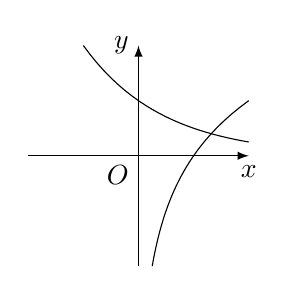
\begin{tikzpicture}[scale = 0.7, >=latex]
    \draw [->] (-2,0) -- (2,0) node [below] {$x$};
    \draw [->] (0,-2) -- (0,2) node [left] {$y$};
    \draw (0,0) node [below left] {$O$};
    \draw [domain = -1:2] plot (\x, {pow(0.5,\x)});
    \draw [domain = -1:2] plot ({pow(0.5,\x)},-\x);
\end{tikzpicture}}
{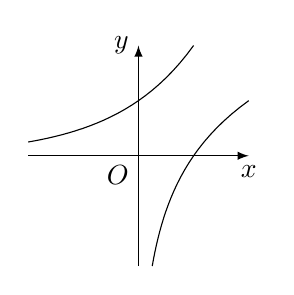
\begin{tikzpicture}[scale = 0.7, >=latex]
    \draw [->] (-2,0) -- (2,0) node [below] {$x$};
    \draw [->] (0,-2) -- (0,2) node [left] {$y$};
    \draw (0,0) node [below left] {$O$};
    \draw [domain = -1:2] plot (-\x, {pow(0.5,\x)});
    \draw [domain = -1:2] plot ({pow(0.5,\x)},-\x);
\end{tikzpicture}}{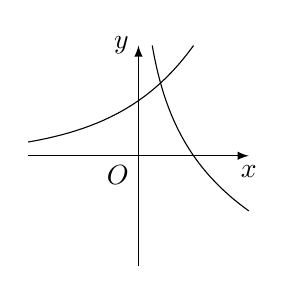
\begin{tikzpicture}[scale = 0.7, >=latex]
    \draw [->] (-2,0) -- (2,0) node [below] {$x$};
    \draw [->] (0,-2) -- (0,2) node [left] {$y$};
    \draw (0,0) node [below left] {$O$};
    \draw [domain = -1:2] plot (-\x, {pow(0.5,\x)});
    \draw [domain = -1:2] plot ({pow(0.5,\x)},\x);
\end{tikzpicture}}{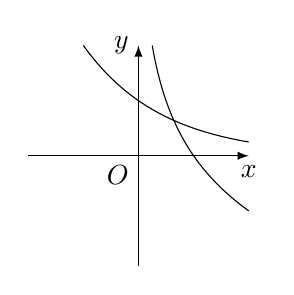
\begin{tikzpicture}[scale = 0.7, >=latex]
    \draw [->] (-2,0) -- (2,0) node [below] {$x$};
    \draw [->] (0,-2) -- (0,2) node [left] {$y$};
    \draw (0,0) node [below left] {$O$};
    \draw [domain = -1:2] plot (\x, {pow(0.5,\x)});
    \draw [domain = -1:2] plot ({pow(0.5,\x)},\x);
\end{tikzpicture}}
\item {\tiny (008095)}函数$f(x)=4+\log _a(x-1)(a>0a\ne 1)$的图像恒经过定点$P$, 则点$P$的坐标是\bracket{20}.
\fourch{$(1, 4)$}{($4, 1)$}{$(2, 4)$}{$(4, 2)$}
\item {\tiny (008096)}已知$0<a<1$, 化简$\sqrt {\lg ^2a-\lg \dfrac{a^2}{10}}$.
\item {\tiny (008097)}已知$\alpha$、$\beta$是方程$\lg ^2x-\lg x-2=0$的两根, 求$\log _{\alpha }\beta +\log _{\beta }\alpha$的值.
\item {\tiny (008363)}如果已知$f(x)=2^{-x}$, 则$f(\log _23)=$\blank{50}.
\item {\tiny (008365)}若$\log _x\dfrac 45<1$, 则$x$的取值范围为\blank{50}.
\item {\tiny (008366)}函数$y=\dfrac 1{\sqrt {\log _{\frac 12}(2-x)}}$的定义域是\blank{50}.
\item {\tiny (008371)}在同一坐标系内作出的两个函数图像如图所示, 这两个函数为\bracket{20}.
\begin{center}
    \begin{tikzpicture}[>=latex]
        \draw [->] (-2,0) -- (2,0) node [below] {$x$};
        \draw [->] (0,-2) -- (0,2) node [left] {$y$};
        \draw (0,0) node [below left] {$O$};
        \draw [domain = -1:2] plot (\x,{pow(2,-\x)});
        \draw [domain = -1:2] plot ({-pow(2,-\x)},-\x);
        \draw (0,1) node [above right] {$1$};
        \draw (-1,0) node [below left] {$-1$};
    \end{tikzpicture}
\end{center}
\twoch{$y=a^x$和$y=\log _a(-x)$}{$y=a^x$和$y=\log _ax^{-1}$}{$y=a^{-x}$和$y=\log _ax^{-1}$}{$y=a^{-x}$和$y=\log _a(-x)$}
\item {\tiny (008372)}若$0<x<\dfrac{\pi}4$, 且$\lg (\sin x+\cos x)=\dfrac 12(3\lg 2-\lg 5)$, 则$\cos x-\sin x$的值为\bracket{20}.
\fourch{$\dfrac{\sqrt 6}3$}{$\dfrac{\sqrt 3}2$}{$\dfrac{\sqrt {10}}5$}{$\dfrac{\sqrt 5}4$}
\item {\tiny (008375)}解方程: $\log _3(x-1)=\log _9(x+5)$.
\item {\tiny (008376)}解方程: $\log _2(9^x-5)=\log _2(3^x-2)+2$.
\item {\tiny (008378)}已知函数$f(x)=\log _2(2^x-1)$.\\
(1) 求$f(x)$的定义域;\\
(2) 判断$f(x)$的增减性, 说明理由;\\
(3) 求$f^{-1}(x)$.
\item {\tiny (008388)}若$\log_m 3<\log_n 3<0$, 则$m,n$满足的条件是\bracket{20}.
\fourch{$m>n>1$}{$n>m>1$}{$0<m<n<1$}{$0<n<m<1$}
\item {\tiny (008389)}若$\log _3x=\cos x$解的个数有\bracket{20}.
\fourch{$0$}{$1$}{$2$}{$3$}
\item {\tiny (008391)}若$\lg a\lg b$是方程$2x^2-4x+1=0$的两个根, 则$(\lg \dfrac ab)^2$的值等于\blank{50}.
\item {\tiny (008392)}定义在$\mathbf{R}$上的偶函数$f(x)$在$[0,+\infty)$上是增函数, 且$f(\dfrac 12)=0$, 则满足$f(\log _{\dfrac 14}x)>0$的$x$的值范围是\blank{50}.
\item {\tiny (008394)}已知函数$f(x)=\log _a\dfrac{x+b}{x-b}(a>0,b>0, a\ne 1)$.\\
(1) 求$f(x)$的定义域;\\
(2) 判断$f(x)$的奇偶性;\\
(3) 求函数$y=f^{-1}(x)$的解析式.
\item {\tiny (009473)}用有理数指数幂的形式表示下列各式(其中$a>0$):\\
(1) $a^{\frac{10}3}\cdot \sqrt[5]{a^3}$;\\
(2) $\sqrt[3]{a\sqrt[3]{a}}$.
\item {\tiny (009476)}以下对数式中, 与指数式$5^x=6$等价的是\bracket{20}.
\fourch{$\log_56=x$}{$\log_5x=6$}{$\log_6x=5$}{$\log_x6=5$}
\item {\tiny (009477)}求下列各式的值:\\
(1) $\log_525$;\\
(2) $\log_{\frac 13}27$;\\
(3) $\log_4\sqrt 2$;\\
(4) $2^{\log_23}$.
\item {\tiny (009478)}求下列各式中$x$的值:\\
(1) $\log_4x=2$;\\
(2) $\log_x4=2$.
\item {\tiny (009479)}已知$A=\log_ax$, $B=\log_ay$($a>0$且$a\ne 1$). 用$A$及$B$表示下列各式:\\
(1) $\log_axy$;\\
(2) $\log_ax^2\sqrt y$.
\item {\tiny (009480)}求下列各式的值:\\
(1) $\log_{15}3+\log_{15}5$;\\
(2) $\log_2\sqrt[3]{4}$;\\
(3) $\log_5\sqrt{10}-\dfrac 12\log_5250$.
\item {\tiny (009481)}已知$\log_73=a$, $7^b=2$. 用$a$及$b$表示$\log_772$.
\item {\tiny (009482)}求下列各式的值:\\
(1) $\log_8\dfrac 14$;\\
(2) $\log_ab\cdot\log_bc\cdot\log_ca$($a$、$b$、$c$均为不等于$1$的正数);\\
(3) $3^{2+\log_94}$;\\
(4) $\dfrac{\log_52\times\log_79}{\log_5\dfrac 13\times\log_72}$.
\item {\tiny (009483)}已知$\log_32=a$, 用$a$表示$\log_296$.
\item {\tiny (009484)}设$a$、$b$是两个不等于$1$的正数, 求证: $\log_ba=\dfrac1{\log_ab}$.
\item {\tiny (009485)}若幂函数$y=x^a$的图像经过点$(3, \sqrt 3)$, 求此幂函数的表达式.
\item {\tiny (009487)}若幂函数$y=x^{-m^2+2m+3}$($m$为整数)的定义域为$\mathbf{R}$, 求$m$的值.
\item {\tiny (009491)}判断下列函数哪些是指数函数, 哪些是幂函数:\\
(1) $y=x$;\\
(2) $y=x^3$;\\
(3) $y=\mathrm{e}^x$;\\
(4) $y=\sqrt[3]{x}$;\\
(5) $y=2^{-x}$;\\
(6) $y=2^x$.
\item {\tiny (009492)}求下列函数的定义域:\\
(1) $y=3^x$;\\
(2) $y=3^{\frac 1{x-2}}$.
\item {\tiny (009493)}在同一平面直角坐标系中分别作出下列函数的大致图像:\\
(1) $y=4^x$;\\
(2) $y=(\dfrac 14)^x$.
\item {\tiny (009495)}已知$a>0$且$a\ne 1$. 若$m>n$, 且$a^m<a^n$, 求实数$a$的取值范围.
\item {\tiny (009496)}求下列不等式的解集:\\
(1) $3^x>3^{0.5}$;\\
(2) $0.2^x<25$.
\item {\tiny (009497)}已知指数函数$y=a^x$($0<a<1$)在区间$[1, 2]$上的最大值比最小值大$\dfrac a3$, 求实数$a$的值.
\item {\tiny (009499)}若对数函数$y=\log a_x$($a>0$且$a\ne 1$)的图像经过点$(4, 2)$, 求此对数函数的表达式.
\item {\tiny (009500)}求下列函数的定义域:\\
(1) $y=\log_2\dfrac{2+x}{1-x}$;\\
(2) $y=\log_a(4-x^2)$(常数$a>0$且$a\ne 1$).
\item {\tiny (009501)}在同一平面直角坐标系中作出$y=\lg x$及$y=\log_{0.1}x$的大致图像.
\item {\tiny (009502)}已知常数$a>0$且$a\ne 1$, 假设无论$a$取何值, 函数$y=\log_a(x-1)$的图像恒经过一个定点, 求此点的坐标.
\item {\tiny (009503)}利用对数函数的性质, 比较下列各题中两个对数的大小:\\
(1) $\log_{0.2}3$和$\log_{0.2}6$;\\
(2) $\log_{0.2}3$和$\log_{0.3}3$.
\item {\tiny (009504)}设$0<a<1$, 求证: 对数函数$y=\log_ax$在区间$(0, +\infty)$上是严格减函数.
\item {\tiny (009506)}利用对数函数的单调性来估算对数$\log_25$的第一位小数的值.
\item {\tiny (009508)}下列四组函数中, 同组的两个函数是相同函数的是\bracket{20}.
\twoch{$y=|x|$与$y=(\sqrt x)^2$}{$y=x$与$y=\mathrm{e}^{\ln x}$}{$y=x$与$y=\sqrt[5]{x^5}$}{$y=x$与$y=(\dfrac 1x)^{-1}$}
\item {\tiny (009509)}求下列函数的值域:\\
(1) $y=(\lg x)^2+1$, $x\in (0, +\infty)$;\\
(2) $y=3x^2-4x+1$, $x\in [0, 1]$.
\item {\tiny (009514)}证明下列函数是奇函数:\\
(1) $y=2^x-2^{-x}$;\\
(2) $y=\log_2(1+x)-\log_2(1-x)$.
\item {\tiny (009523)}求函数$y=(\dfrac 12)^x$, $x\in [1, 3]$的最大值与最小值.
\item {\tiny (009530)}用函数的观点解不等式: $2^x+\log_2x>2$.
\item {\tiny (009908)}借助函数图像, 判断下列导数的正负(可利用信息技术工具):\\
(1) $f'(\dfrac\pi 4)$, 其中$f(x)=\sin x$;\\
(2) $f'(0)$, 其中$f(x)=(\dfrac 12)^x$.
\item {\tiny (009912)}证明函数$y=\ln x$与$y=\mathrm{e}^x$没有驻点.
\item {\tiny (009913)}求下列函数$y=f(x)$的导数, 其中:\\
(1) $f(x)=3\mathrm{e}^x-x^{\mathrm{e}}+\mathrm{e}$;\\
(2) $f(x)=\cos x-\dfrac 2x$;\\
(3) $f(x)=(2x+1)^3$;\\
(4) $f(x)=\sqrt x\sin x$;\\
(5) $f(x)=x\ln x-\dfrac1{x^2}$;\\
(6) $f(x)=\dfrac{x^2-1}x$;\\
(7) $f(x)=\dfrac{x^2-1}{x^2+1}$;\\
(8) $f(x)=\tan x$.
\item {\tiny (009917)}求下列函数的导数:\\
(1) $y=3x \sqrt{2-x}$;\\
(2) $y=\dfrac{\ln(2x+1)}x$.
\item {\tiny (009918)}利用导数研究下列函数的单调性, 并说明所得结果与你之前的认识是否一致:\\
(1) $y=\mathrm{e}^x$;\\
(2) $y=\ln x$;\\
(3) $y=ax^2+bx+c$, 其中$a\ne 0$.
\item {\tiny (009919)}确定下列函数的单调区间:\\
(1) $y=x\mathrm{e}^x$;\\
(2) $y=4x^3-9x^2+6x+7$.
\item {\tiny (010001)}已知$f(x)=\log_3(x+a)+\log_3(6-x)$.\\
(1) 若将函数$y=f(x)$的图像向下平移$m$($m>0$)个单位后, 所得的图像经过点$(3,0)$与点$(5,0)$, 求$a$与$m$的值;\\
(2) 若$a>-3$且$a\ne 0$, 解关于$x$的不等式$f(x)\le f(6-x)$.
\item {\tiny (010107)}用有理数指数幂的形式表示下列各式(其中$x>0$, $y>0$):\\
(1) $\sqrt[3]{5}$;\\
(2) $(\sqrt[5]{x})^3$;\\
(3) $\sqrt[7]{x^3y^4}$;\\
(4) $\sqrt[7]{\dfrac{x^3}{y^4}}$.
\item {\tiny (010110)}用有理数指数幂的形式表示下列各式(其中$a>0$, $b>0$):\\
(1) $a^\frac 13a^\frac 14$;\\
(2) $\sqrt[3]{a\sqrt a}$;\\
(3) $(a^\frac 14b^{-\frac 38})^8$;\\
(4) $(\dfrac {a^{-3}b^4}{\sqrt b})^{-\frac 13}$.
\item {\tiny (010113)}设$a^{2x}=2$, 且$a>0$. 求$\dfrac{a^{3x}+a^{-3x}}{a^x+a^{-x}}$的值.
\item {\tiny (010114)}设$a>b>0$, 求证: $a^ab^b>(ab)^\frac{a+b}2$.
\item {\tiny (010115)}把下列指数式写成对数式:\\
(1) $3^4=81$;\\
(2) $5^{-\frac1 2}=x$.
\item {\tiny (010116)}将下列对数式写成指数式:\\
(1) $\log_{\frac 13}27=-3$;\\
(2) $\log_2\dfrac 18=-3$.
\item {\tiny (010117)}求下列各式的值:\\
(1) $\log_3 27$;\\
(2) $\log_{\frac 12}8$;\\
(3) $\ln \dfrac 1{\mathrm{e}}+\lg \sqrt {10}$.
\item {\tiny (010118)}求下列各式中$x$的值:\\
(1) $\log_2x=5$;\\
(2) $\log_{\sqrt 5}\dfrac1{125}=x$;\\
(3) $\log_x4=\dfrac 12$.
\item {\tiny (010119)}求下列各式的值:\\
(1) $\log_2(2\times 3\sqrt 2)$;\\
(2) $\log_{21}3+\log_{21}7$;\\
(3) $\log_5\sqrt 6-\dfrac 12\log_5 150$;\\
(4) $3^{\log_31}+\log_248-\log_23$;\\
(5) $3\log_3\dfrac 32-\log_3\dfrac 74+\dfrac 12\log_34+\log_37$.
\item {\tiny (010120)}已知$A=\log_ax$, $B=\log_ay$, $C=\log_az$($a>0$且$a\ne 1)$. 用$A$、$B$及$C$表示下列各式:\\
(1) $\log_a(xy^2)$;\\
(2) $\log_a\dfrac{xy}{\sqrt z}$;\\
(3) $\log_a(x^2y^2)+\log_a(y\sqrt x)$.
\item {\tiny (010121)}求下列各式的值:\\
(1) $\log_42\sqrt 2$;\\
(2) $\log_23\times \log_92$;\\
(3) $\dfrac 3{\log_26}+\dfrac 3{\log_36}$;\\
(4) $(\log_43+\log_83)(\log_32+\log_92)+\log_{\frac 12}\sqrt[4]{32}$.
\item {\tiny (010122)}已知$a=\lg 5$, 用$a$表示$\lg 2$和$\lg$ $20$.
\item {\tiny (010123)}求下列各式中$x$的取值范围:\\
(1) $\log_2(1-3x)$;\\
(2) $\log_a(x^2+x)$($a>0$且$a\ne 1)$.
\item {\tiny (010124)}求下列各式的值:\\
(1) $\log_48-\log_{\frac 19}3-\log_{\sqrt 2}4$;\\
(2) $2^{\log_65}\times 3^{\log_65}$;\\
(3) $(\lg 50)^2+\lg 2\times \lg 50^2+(\lg 2)^2$.
\item {\tiny (010125)}科学家以里氏震级来度量地震的强度, 若设$I$为地震时所散发出来的相对能量程度, 则里氏震级度量$r$可定义为$r=\dfrac 23\lg I+2$. 求$7.8$级地震和$6. 9$级地震的相对能量比值. (结果精确到个位)
\item {\tiny (010126)}已知$\lg 2=a$, $\lg 3=b$. 用$a$及$b$表示$\log_2 3$及$\log_{12}25$.
\item {\tiny (010127)}已知$5.4^x=3$, $0.6^y=3$. 求$\dfrac 1x-\dfrac 1y$的值.
\item {\tiny (010128)}设$a$、$b$、$c$、$d$均为正数, 且$a$、$c$均不为$1$. 求证:
$\log_ab\cdot \log_cd=\log_ad\cdot \log_cb$.
\item {\tiny (010129)}若幂函数$y=x^a$的图像经过点$(\sqrt[4]{3}, 3)$, 求此幂函数的表达式.
\item {\tiny (010133)}下列幂函数在区间$(0, +\infty)$上是严格增函数, 且图像关于原点成中心对称的是\blank{50}(请填入全部正确的序号).\\
\textcircled{1} $y=x^\frac 12$; \textcircled{2} $y=x^\frac 13$; \textcircled{3} $y=x^\frac 23$; \textcircled{4} $y=x^{-\frac 13}$.
\item {\tiny (010135)}幂函数$y=x^{n(n+1)}$($n$为正整数)的图像一定经过\blank{50}象限.
\item {\tiny (010136)}若幂函数$y=x^s$在$0<x<1$时的图像位于直线$y=x$的上方, 则$s$的取值范围是\blank{50}.
\item {\tiny (010137)}下列命题中, 正确的是\bracket{20}.
\onech{当$n=0$时, 函数$y=x^n$的图像是一条直线}{幂函数$y=x^n$的图像都经过$(0, 0)$和$(1, 1)$两个点}{若幂函数$y=x^n$的图像关于原点成中心对称, 则$y=x^n$在区间$(-\infty, 0)$上是严格增函数}{幂函数的图像不可能在第四象限}
\item {\tiny (010138)}写出一个图像经过第一、第二象限但不经过原点的幂函数的表达式.
\item {\tiny (010140)}下列函数是指数函数的序号为\blank{50}(请填入全部正确的序号).\\
\textcircled{1} $y=(-4)^x$; \textcircled{2} $y=(\dfrac 14)^x$; \textcircled{3} $y=4^x$; \textcircled{4} $y=x^{-4}$; \textcircled{5} $y=(\sqrt 4)^x$.
\item {\tiny (010142)}在同一直角坐标系中作出下列函数的大致图像, 并指出这些函数图像间的关系:\\
(1) $y=(\dfrac 32)^x$;\\
(2) $y=(\dfrac 23)^x$;\\
(3) $y=(\dfrac 23)^x-1$.
\item {\tiny (010143)}已知指数函数$y=(m-2)^x$在$\mathbf{R}$上是严格减函数, 求实数$m$的取值范围.
\item {\tiny (010147)}已知指数函数$y=a^x$($a>0$且$a\ne 1)$在区间$[1, 2]$上的最大值与最小值之和等于$6$, 求实数$a$的值.
\item {\tiny (010149)}在同一平面直角坐标系中, 指数函数$y=a^x$($a>0$且$a\ne 1$)和一次函数$y=a(x+1)$的图像关系可能是\bracket{20}.
\fourch{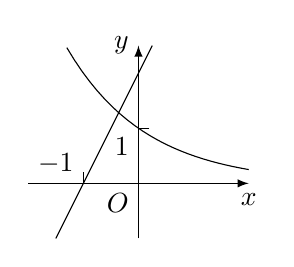
\begin{tikzpicture}[>=latex,scale=0.7]
\draw [->] (-2,0) -- (2,0) node [below] {$x$};
\draw [->] (0,-1) -- (0,2.5) node [left] {$y$};
\draw (0,0) node [below left] {$O$};
\draw [domain = -2:1.3] plot (-\x,{pow(2,\x)});
\draw (-1.5,-1) -- (0.25,2.5);
\draw (0.2,1) -- (0,1) node [below left] {$1$};
\draw (-1,0.2) -- (-1,0) node [above left] {$-1$};
\end{tikzpicture}}{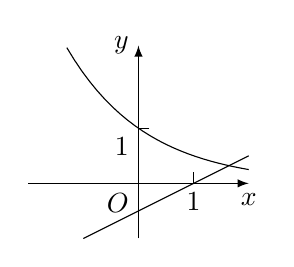
\begin{tikzpicture}[>=latex,scale=0.7]
\draw [->] (-2,0) -- (2,0) node [below] {$x$};
\draw [->] (0,-1) -- (0,2.5) node [left] {$y$};
\draw (0,0) node [below left] {$O$};
\draw [domain = -2:1.3] plot (-\x,{pow(2,\x)});
\draw (-1,-1) -- (2,0.5);
\draw (0.2,1) -- (0,1) node [below left] {$1$};
\draw (1,0.2) -- (1,0) node [below] {$1$};
\end{tikzpicture}}{\begin{tikzpicture}[>=latex,scale=0.7]
\draw [->] (-2,0) -- (2,0) node [below] {$x$};
\draw [->] (0,-1) -- (0,2.5) node [left] {$y$};
\draw (0,0) node [below left] {$O$};
\draw [domain = -2:1.3] plot (\x,{pow(2,\x)});
\draw (-1.5,-1) -- (0.25,2.5);
\draw (0.2,1) -- (0,1) node [below right] {$1$};
\draw (-1,0.2) -- (-1,0) node [below left] {$-1$};
\end{tikzpicture}}{\begin{tikzpicture}[>=latex,scale=0.7]
\draw [->] (-2,0) -- (2,0) node [below] {$x$};
\draw [->] (0,-1) -- (0,2.5) node [left] {$y$};
\draw (0,0) node [below left] {$O$};
\draw [domain = -2:1.3] plot (\x,{pow(2,\x)});
\draw (-2,-0.5) -- (2,1.5);
\draw (0.2,1) -- (0,1) node [above left] {$1$};
\draw (-1,0.2) -- (-1,0) node [below] {$-1$};
\end{tikzpicture}}
\item {\tiny (010150)}如图所示的是某池塘中的浮萍蔓延的面积$y$(单位: $\text{m}^2$)与时间$t$(单位: 月)的关系: $y=a^t$($a>0$且$a\ne 1)$. 
\begin{center}
\begin{tikzpicture}[>=latex,scale = 0.5]
\draw [->] (0,0) -- (4,0) node [below] {$t/\text{月}$};
\draw [->] (0,0) -- (0,9) node [left] {$y/\text{m}^2$};
\draw (0,0) node [below left] {$O$};
\draw [domain = 0:3.1] plot (\x,{pow(2,\x)});
\foreach \i in {1,2,3}{\draw [dashed] (\i,0) -- (\i,{pow(2,\i)}) -- (0,{pow(2,\i)}); \draw (\i,0) node [below] {$\i$};};
\foreach \i in {2,4,8}{\draw (0,\i) node [left] {$\i$};};
\end{tikzpicture}
\end{center}
以下结论:
\textcircled{1} 这个指数函数的底数是$2$; 
\textcircled{2} 第$5$个月时, 浮萍的面积就会超过$30\text{m}^2$;
\textcircled{3} 浮萍面积从$4\text{m}^2$到$12\text{m}^2$需要经过$1.5$个月;
\textcircled{4} 浮萍每个月增加的面积都相等. 其中, 正确结论的序号是\bracket{20}.
\fourch{\textcircled{1}\textcircled{2}\textcircled{3}}{\textcircled{1}\textcircled{2}\textcircled{3}\textcircled{4}}{\textcircled{2}\textcircled{3}\textcircled{4}}{\textcircled{1}\textcircled{2}}
\item {\tiny (010151)}若$x>0$时, 指数函数$y=(a^2-1)^x$的值总大于$1$, 求实数$a$的取值范围.
\item {\tiny (010152)}若$-1<x<0$, 比较$3^x, 3^{-x}$及$3^{2x}$的大小.
\item {\tiny (010155)}求下列函数的定义域:\\
(1) $y=\log_a (x+12)$(常数$a>0$且$a\ne 1$);\\
(2) $y=\log_2\dfrac1{x^2-2x+5}$.
\item {\tiny (010156)}已知对数函数$y=\log_ax$($a>0$且$a\ne 1)$的图像经过点$(3, 2)$. 若点$P(b, 4)$为此函数图像上的点, 求实数$b$的值.
\item {\tiny (010157)}在同一平面直角坐标系中画出下列函数的图像, 并指出这些函数图像之间的关系.\\
(1) $y=\log_3x$;\\
(2) $y=\log_{\frac 13}x$;\\
(3) $y=(\dfrac 13)^x$.
\item {\tiny (010158)}已知常数$a>0$且$a\ne 1$, 假设无论$a$取何值, 函数$y=\log_ax-1$的图像恒经过一个定点. 求此点的坐标.
\item {\tiny (010159)}根据下列不等式, 确定底数$a$的取值范围:\\
(1) $\log_a 0.2<\log_a 0.1$;\\
(2) $\log_a\pi >\log_a\mathrm{e}$.
\item {\tiny (010160)}已知$y=\log_{a^2-1}x$在区间$(0, +\infty)$上是严格减函数, 求实数$a$的取值范围.
\item {\tiny (010161)}已知对数函数$y=\log_ax$($a>1$)在区间$[1, 2]$上的最大值比最小值大$1$, 求$a$的值.
\item {\tiny (010162)}若$a>b>c>1$, 则下列不等式不成立的是\blank{50}. (填写所有不成立的不等式的序号)\\
\textcircled{1} $\log_ab>\log_ac$; \textcircled{2} $\log_a\dfrac 1b>\log_a\dfrac 1c$; \textcircled{3} $\log_{\frac 1a}b>\log_{\frac 1a}c$; \textcircled{4} $\log_{\frac 1a}\dfrac 1b>\log_{\frac 1a}\dfrac 1c$.
\item {\tiny (010163)}设常数$a>0$且$a\ne 1$, 求函数$y=\log_a(a-a^x)$的定义域.
\item {\tiny (010164)}根据下列不等式, 比较正数$m$及$n$的大小:\\
(1) $\log_3m<\log_3n$;\\
(2) $\log_am<\log_an$($a>0$且$a\ne 1$);\\
(3) $\log_mN<\log_nN$($0<m<1$, $0<n<1$, $0<N<1$).
\item {\tiny (010165)}设$0<a<1$, 若$\log_a(4x^2-1)<\log_a(-2x^2+x+1)$, 求实数$x$的取值范围.
\item {\tiny (010168)}求下列函数的定义域:\\
(1) $y=\dfrac1{x^2+2x-3}$;\\
(2) $y=\sqrt{4-3x-x^2}$;\\
(3) $y=\sqrt{x-2}+\sqrt{x+3}$;\\
(4) $y=\dfrac 1{\lg(x+2)}+\dfrac 1{\sqrt{5-x}}$.
\item {\tiny (010174)}证明下列函数$y=f(x)$为偶函数:\\
(1) $f(x)=x^2+x^{-2}$;\\
(2) $f(x)=\dfrac{x(2^x-1)}{2^x+1}$.
\item {\tiny (010175)}证明下列函数$y=f(x)$为奇函数:\\
(1) $f(x)=x^{-3}$;\\
(2) $f(x)=\dfrac{\mathrm{e}^x-\mathrm{e}^{-x}}2$
\item {\tiny (010176)}判断下列函数$y=f(x)$的奇偶性, 并说明理由:\\
(1) $f(x)=2x+\sqrt[3]x$;\\
(2) $f(x)=2x^4-x^2$;\\
(3) $f(x)=x^2-x$;\\
(4) $f(x)=\dfrac{1-x}{1+x}$;\\
(5) $f(x)=\lg\dfrac {1-x}{1+x}$.
\item {\tiny (010178)}证明:函数$y=\lg (1-x)$在其定义域上是严格减函数.
\item {\tiny (010180)}求函数$y=\log_{\frac 12}(x+2)$, $x\in [2, 6]$的最大值与最小值.
\item {\tiny (010183)}判断下列函数$y=f(x)$的奇偶性, 并说明理由:\\
(1) $f(x)=\dfrac{10^x-10^{-x}}{10^x+10^{-x}}$;\\
(2) $f(x)=x(\dfrac 1{2^x-1}+\dfrac 12)$.
\item {\tiny (010196)}证明: 方程$\lg x+2x=16$没有整数解.
\item {\tiny (010200)}求下列函数的反函数:\\
(1) $y=10^x+1$;\\
(2) $y=\log_2(x+1)$;\\
(3) $y=\log_2(2x)$.
\item {\tiny (010201)}已知$f(x)=1-\log_2x$, 设$y=f^{-1}(x)$是$y=f(x)$的反函数. 求$f^{-1}(-3)$的值.
\item {\tiny (010795)}借助函数图像, 判断下列导数的正负:\\
(1) $f'(-\dfrac \pi 4)$, 其中$f(x)=\cos x$;\\
(2) $f'(3)$, 其中$f(x)=\ln x$.
\item {\tiny (010805)}求下列函数$y=f(x)$的导数:\\
(1) $f(x)=2x^{\mathrm{e}}-\mathrm{e}^2$;\\
(2) $f(x)=\mathrm{e}^x\cos x$;\\
(3) $f(x)=\dfrac{x-1}{x-2}$;\\
(4) $f(x)=\dfrac{\ln x}{\sin x}$.
\item {\tiny (010813)}直线$y=-x+b$是下列函数的切线吗? 如果是, 请求出$b$的值; 如果不是, 请说明理由.\\
(1) $y=\ln x$;\\
(2) $y=\dfrac 1x$.
\item {\tiny (010815)}判断下列求导结果是否正确. 如果不正确, 请指出错在哪里, 并予以改正.\\
(1) $(\dfrac{\sin x}x)'=-\dfrac 1{x^2}\sin x-\dfrac{\cos x}x$;\\
(2) $(\ln (2-x))'=\dfrac 1{2-x}$.
\item {\tiny (010818)}求下列函数$y=f(x)$的导数, 其中:\\
(1) $f(x)=x^2\sin 3x-\dfrac 2{\sqrt x}$;\\
(2) $f(x)=\dfrac{\mathrm{e}^x-\mathrm{e}^{-x}}{\mathrm{e}^x+\mathrm{e}^{-x}}$.
\item {\tiny (010819)}利用导数研究下列函数的单调性, 并说明结果与你之前的认识是否一致:\\
(1) $y=(\dfrac 1{\mathrm{e}})^x$;\\
(2) $y=\log_{\frac 1{\mathrm{e}}}x$.
\item {\tiny (010822)}求下列函数的单调区间、极值点和极值:\\
(1) $y=x^2+2x+3$;\\
(2) $y=x+\dfrac 1x$;\\
(3) $y=3x-x^3$;\\
(4) $y=x^2\mathrm{e}^x$.
\item {\tiny (010827)}判断下列函数在$(-\infty, +\infty)$上是否存在驻点, 是否存在极值点, 并说明理由:\\
(1) $y=x^n$, $n$为正奇数;\\
(2) $y=x^n$, $n$为正偶数.
\end{enumerate}



\end{document}